%\VignetteIndexEntry{distr - manual}
%\VignetteDepends{startupmsg,distr}
%\VignetteKeywords{probability distribution,simulation,estimation}
%\VignettePackage{distr}
%
\documentclass[11pt]{article}
\usepackage{geometry}\usepackage{color}
\usepackage{ifpdf}
\definecolor{darkblue}{rgb}{0.0,0.0,0.75}
\usepackage{amssymb}
\usepackage[%
baseurl={http://www.bioconductor.org},%
pdftitle={S4 Classes for Distributions---a manual for packages distr, distrSim, distrTEst, distrEx,
distrMod, and distrTeach},%
pdfauthor={Peter Ruckdeschel, Matthias Kohl, Thomas Stabla, Florian Camphausen},%
pdfsubject={distr},%
pdfkeywords={probability distribution,simulation,estimation},%
pagebackref,bookmarks,colorlinks,linkcolor=darkblue,citecolor=darkblue,%
pagecolor=darkblue,raiselinks,plainpages,pdftex]{hyperref}
%
\usepackage{Sweave}
\markboth{\sl Packages ``{\tt distr}'', ``{\tt distrSim}'', ``{\tt distrTEst}'',
``{\tt distrEx}'', ``{\tt distrTeach}'', ``{\tt distrMod}''}%
{\sl Packages ``{\tt distr}'', ``{\tt distrSim}'', ``{\tt distrTEst}'',
``{\tt distrEx}'', ``{\tt distrTeach}'', ``{\tt distrMod}''}
%
% -------------------------------------------------------------------------------
\newcommand{\code}[1]{{\tt #1}}
\newcommand{\pkg}[1]{{\tt "#1"}}
\newcommand{\pkgversion}{{\tt 2.0}}
\newcommand{\pkgExversion}{{\tt 2.0}}
\newcommand{\Reals}{\mathbb{R}}
\newcommand{\R}{\mathbb{R}}
\newcommand{\N}{\mathbb{N}}
% -------------------------------------------------------------------------------
% new from version 2.5 of R:
% -------------------------------------------------------------------------------

% -------------------------------------------------------------------------------
%
% -------------------------------------------------------------------------------
\begin{document}
% -------------------------------------------------------------------------------
\title{{\tt S4} Classes for Distributions---a manual for packages \pkg{distr},
        \pkg{distrEx}, \pkg{distrMod}, \pkg{distrSim}, \pkg{distrTEst}, \pkg{distrTeach},
        version \pkgversion}
%,version \pkgExversion}
\author{\small Peter Ruckdeschel\thanks{Fraunhofer ITWM, Kaiserslautern}
\\[-.5ex]
\small Matthias Kohl\thanks{Universit\"at Bayreuth}
\\[-.5ex]
\small Thomas Stabla\thanks{Hans-Sachs-Gymnasium N\"urnberg}
\\[-.5ex]
\small Florian Camphausen\thanks{West-LB, D\"usseldorf}
\smallskip\\
\small Fraunhofer ITWM\\[-.5ex]
\small Fraunhofer Platz 1\\[-.5ex]
\small D-95440 Kaiserslautern\\[-.5ex]
\small Germany\\
\small e-Mail: {\small \tt Peter.Ruckdeschel@itwm.fraunhofer.de}\\
}
\maketitle
% -------------------------------------------------------------------------------
\begin{abstract}
% -------------------------------------------------------------------------------
\pkg{distr} is a package for {\sf R} from version {\tt 1.8.1} onwards that is
distributed under {\tt GPL} license 2.0. Its own current version is \pkgversion.
%
The aim of this package is to provide a conceptual treatment of random variables
(r.v.'s) by means of {\tt S4}--classes. A mother class \code{Distribution} is
introduced with slots for a parameter and for functions {\tt r},  {\tt d},
{\tt p}, and {\tt q} for simulation, respectively for evaluation of density /
c.d.f.\ and quantile function of the corresponding distribution. All
distributions of the \pkg{stats} package are implemented as subclasses of either
\code{AbscontDistribution} or \code{DiscreteDistribution},
which themselves are again subclasses of \code{UnivariateDistribution}. %\\
%
By means of these classes, we may automatically generate new objects of these
classes for the laws of r.v.'s under standard mathematical univariate
transformations and under standard bivariate arithmetical operations acting
on independent r.v.'s.
%
%From version 1.6 on, \pkg{distr} has been split up into the smaller packages
%\pkg{distr} (only distribution-classes and -methods),  \pkg{distrSim}
%(standardized treatment of simulations, also under contaminations)
%and \pkg{distrTEst} \newline(classes and methods for evaluations of statistical
%procedures on such simulations).
Package \pkg{distr} in this setting works as basic package for further extensions.
These start with package \pkg{distrEx}, covering statistical functionals like
expectation, variance and the median evaluated at distributions, as well as
distances between distributions and basic support for multivariate and
conditional distributions. Next, from version 2.0 on, comes package \pkg{distrMod}
which uses these concepts to provide an object orientated competitor to
\code{fitdistr} from package \pkg{MASS} in covering estimation in statistical
models. Further on there are packages \pkg{distrSim} for the standardized
treatment of simulations, also under contaminations and package
\pkg{distrTEst} with classes and methods for evaluations of statistical
procedures on such simulations. Finally, from version 2.0 on, there is package
\pkg{distrTeach} to embody illustrations for basic stats courses using
our distribution classes.

%\noindent The latter two of them require package \pkg{setRNG} by
%\href{mailto:pgilbert@bank-banque-canada.ca}{Paul Gilbert}
%to be installed from \href{http://cran.r-project.org/mirrors.html}{\tt CRAN}.
% \\

%\noindent Additionally, mainly contributed by \cite{MK:05}, in \pkg{distrEx} we
%extend the functionality of \pkg{distr}, providing functionals like expectation
%or variance and distances for distributions. Also, this package contains some
%first steps to multivariate distributions, providing classes for discrete
%multivariate distributions and for factorized, conditional
%distributions.
% -------------------------------------------------------------------------------
\end{abstract}
% -------------------------------------------------------------------------------
\tableofcontents
\noindent
{\small Parts of this document appeared in an earlier and much shorter form in
{\em R-News\/}, {\bf 6}(2) as {\sf ``S4 Classes for Distributions''},
c.f.\ \cite{R:K:S:C:04}, which in its
published form refers to package versions 1.6, resp.\ 0.4-2. This present document
takes into account the subsequent revisions and versions.}\medskip
% -------------------------------------------------------------------------------
\addtocounter{section}{-1}
\section{Motivation}
% -------------------------------------------------------------------------------
{\sf R} up to now contains powerful techniques for virtually
any useful distribution using the suggestive naming convention
{\tt [prefix]<name>} as functions where {\tt [prefix]} stands for
 {\tt r}, {\tt d}, {\tt p}, or {\tt q}
 and {\tt <name>} is the name of the distribution.\\
There are limitations of this concept, however:
You can only use distributions which are implemented in some library
already or for which you yourself have provided an implementation.
In many natural settings you want to formulate algorithms once for
all distributions, so you should be able to treat the actual distribution
{\tt <name>} as sort of a variable.\\
You may of course paste together prefix and the value of {\tt <name>} as a
string and then use \code{eval(parse(....))}. This is neither very elegant nor
flexible, however.\\
%
Instead, we would rather like to implement the algorithm by passing an object of
some distribution class as argument to the function. Even better though, we
would use a generic function and let the {\tt S4}-dispatching mechanism decide
what to do at run-time. In particular, we would like to automatically generate
the corresponding functions {\tt r}, {\tt d}, {\tt p}, and {\tt q} for the law
of expressions like \code{X+3Y} for objects \code{X} and \code{Y} of class
\code{Distribution}, or, more general, of a transformation of $X$, $Y$ under a
function $f\colon \Reals^2 \to \Reals$ which is already realized as a function
in {\sf R}.\\
This is possible with package \pkg{distr}. As an example, try
\begin{Schunk}
\begin{Sinput}
> library(distr)
> N <- Norm(mean = 2, sd = 1.3)
> P <- Pois(lambda = 1.2)
> Z <- 2*N + 3 + P
> Z
\end{Sinput}
\begin{Soutput}
Distribution Object of Class: AbscontDistribution
\end{Soutput}
\begin{Sinput}
> plot(Z, withSweave = TRUE)
> p(Z)(0.4)
\end{Sinput}
\begin{Soutput}
[1] 0.002415384
\end{Soutput}
\begin{Sinput}
> q(Z)(0.3)
\end{Sinput}
\begin{Soutput}
[1] 6.70507
\end{Soutput}
\begin{Sinput}
> Zs <- r(Z)(50)
> Zs
\end{Sinput}
\begin{Soutput}
 [1]  6.343708 10.803157  5.754789  9.343831  5.171048 10.047726 10.650778
 [8]  9.294919  6.631331 13.414423  6.184404  7.486513  9.411807 10.737207
[15] 12.115160 10.613250  4.307291  2.701835 10.216650 10.995756  6.751414
[22] 12.661101  2.183357  9.824653  4.534901 11.171117  5.108571  9.851101
[29]  9.928463  9.311634  5.111554  8.336013 10.276997  5.580951  9.873637
[36]  9.722722  6.387387  9.725926  4.677760  7.104121 11.009944  8.938798
[43] 13.332932  9.988780  7.908832  6.705098  6.154896  4.538273 10.403014
[50]  8.796188
\end{Soutput}
\end{Schunk}
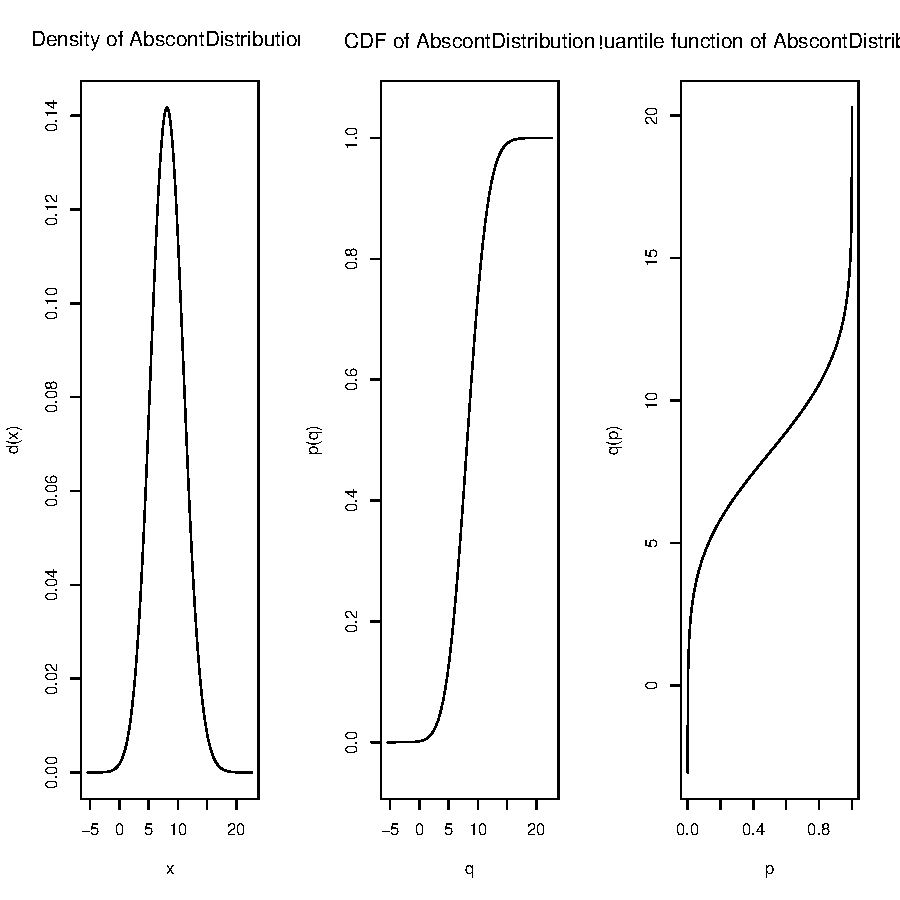
\includegraphics{distr-exam1}
\par
\begin{small}
\noindent{\bf Comment:}\\
Let \code{N} an object of class \code{"Norm"} with parameters  \code{mean=2},
\code{sd=1.3} and let \code{P}  an object of class \code{"Pois"} with parameter
\code{lambda=1.2}. Assigning to \code{Z} the expression \code{2*N+3+P}, a
new distribution object is generated ---of class \code{"AbscontDistribution"} in
our case--- so that identifying \code{N}, \code{P}, \code{Z} with random
variables distributed according to {\tt N}, {\tt P}, {\tt Z},
${\cal L}({\tt Z})={\cal L}(2*{\tt N}+3+{\tt P})$,  and writing \code{p(Z)(0.4)}
we get $P(Z\leq 0.4)$, \code{ q(Z)(0.3)}  the $30\%$-quantile of {\tt Z},
and with \code{r(Z)(50)} we generate $50$ pseudo random numbers distributed
according to {\tt Z}, while the \code{plot} command generates the above figure.
\end{small}
% -------------------------------------------------------------------------------
\section{Concept}
% -------------------------------------------------------------------------------
In developing our packages, we had the following principles in mind:
We wanted to be open in our design so that our classes could easily be extended
by any volunteer in the {\sf R} community to provide more complex classes of
distributions as multivariate distributions, times series distributions,
conditional distributions. As an exercise, the reader is encouraged to implement
extrem value  distributions from the package \pkg{evd}\footnote{a solution to
this ``homework''  may be found in the sources to \pkg{distrEx}}. The largest
effort will in fact be the documentation\ldots\\
We also wanted to preserve naming and notation from {\sf R}-\pkg{stats}
as far as possible so that any programmer used to {\tt S} could quickly
use our package. Even more so, as the distributions already implemented to
{\sf R} are all well tested and programmed with skills we lack, we use the
existing {\tt r}, {\tt d}, {\tt p}, and {\tt q}-functions wherever possible,
only wrapping them by small code sniplets to our class hierarchy.\\
Third we wanted to use a suggestive notation for our automatically generated
methods \code{r}, \code{d}, \code{p}, and \code{q}, which we think is now
largely achieved. All this should make intensive use of object orientation in
order to be able to use inheritance and method overloading.
Let us briefly explain why we decided to realize \code{r}, \code{d},
\code{p}, and \code{q} as part of our class definitions:
Doing so, we place ourselves somewhere between
pure object orientation where methods would be {\it slots\/} ---in the language
of the {\tt S4}-concept, confer \cite{Cham:98}--- and the {\tt S4} paradigm
where methods ``live their own life'' apart from the classes, or, to \code{q},
which should be regarded use \cite{Beng:03}'s terminology, we use
COOP\footnote{class-object-orientated
programming, as e.g.\ in {\tt C++}}-style for \code{r}, \code{d}, \code{p}, and
\code{q} methods, and FOOP\footnote{function-object-orientated programming,
as in the {\tt S4}-concept} -style for "normal" methods.\\
The {\tt S4}-paradigm with methods which are not attached to an object but
rather behave differently according to the classes of their arguments is fine
if there are particular user-written methods for only some few general
distribution classes like  \code{AbscontDistribution}, as in the case for
\code{plot} or \code{"+"} (c.f.\ \cite{K:R:S:04}, Section 2.2).
During a typical {\sf R} session with \pkg{distr}, however, there will be a lot
of, mostly automatically generated objects of our distribution classes, each
with its own \code{r}, \code{d}, \code{p}, and \code{q}; this even applies to
intermediate expressions like \code{2*N}, \code{2*N+3} to eventually produce
\code{Z} in the example in the motivation. Treating \code{r}, \code{d},
\code{p}, and \code{q} as generic functions, we would need to generate new
classes for each expression \code{2*N}, \code{2*N+3}, \code{Z} and,
correspondingly, particular {\tt S4}-methods for \code{r}, \code{d}, \code{p},
and \code{q} for each of these new classes; apparently, this would produce
overly many classes for an effective inheritance structure. \\
In providing arithmetics for distributions, we have to deviate a little from
the paradigm of {\tt S} as a functional language: For operators like ``$+$'',
additional parameters controlling the precision of the results cannot be handily
passed as arguments. For this purpose we provide global options which may be
inspected and modified by \code{distroptions},
\code{getdistrOption}\footnote{Upto version 0.4-4, we used a different mechanism
to inspect/modify global options of \pkg{distrEx} (see
section~\ref{distrExoptions}); corresponding functions \code{distrExoptions},
\code{getdistrExOption} for package \pkg{distrEx} are available from version
1.9 on.} in complete analogy to \code{options}, \code{getOption}.
%
Finally our concept as to parameters: Contrary to the standard {\sf R}-functions
like \code{rnorm} we only permit length $1$ for parameters like \code{mean},
because we see the objects as implementations of univariate random variables,
for which vector-valued parameters make no sense; rather one could gather
several objects with possibly different parameters to a vector/list of
distributions. Of course, the original functions \code{rnorm} etc.\ remain
unchanged and still allow for vector-valued parameters.
Kouros Owzar  in an off-list mail raised the point, that in case of multiple
parameters as in case of the normal or the $\Gamma$-distribution, it might be
useful to be able to pass these multiple parameters in vectorized form to the
generating function. We, too, think that this is a good idea, but have
shifted this question to the new extension package \pkg{distrMod} which covers
more general treatment of statistical models, see section~\ref{distrMod}.
% -------------------------------------------------------------------------------
\section{Organization in classes}
% -------------------------------------------------------------------------------
Loosely speaking we have three large groups of classes: distribution classes (in
\pkg{distr}), simulation classes (in \pkg{distrSim}) and an evaluation class (in
\pkg{distrTEst}), where the latter two are to be considered only as tools which
allow a unified treatment of simulations and evaluation of statistical estimation
(perhaps also tests and predictions later) under varying simulation situations.
Additionally, package \pkg{distrEx} provides classes for discrete multivariate
distributions and for factorized, conditional distributions, as well as a bundle
of functionals and distances (see below).
% -------------------------------------------------------------------------------
\subsection{Distribution classes}
% -------------------------------------------------------------------------------
The purpose of the classes derived from the class \code{Distribution}  is to
implement the concept of a r.v./distribution as such in {\sf R}.\\
All classes derived from \code{Distribution} have a slot \code{param} for a
parameter, a slot \code{img} for the range and the constitutive slots \code{r},
\code{d}, \code{p}, and \code{q}.\\
From version 1.9 on, up to arguments referring to a parameter of the
distribution (like \code{mean} for the normal distribution), these function
slots have the same arguments as those of package \pkg{stats}, i.e.; for a
distribution object \code{X} we may call these functions as

\begin{itemize}
\item \code{r(X)(n)}  $\qquad$ ---except for objects of class \code{Hyper},
where there is a slot \code{n} already, so here the argument name
to \code{r} is \code{nn}.
\item \code{d(X)(x, log = FALSE)}
\item \code{p(X)(q, lower.tail = TRUE, log.p = FALSE)}
\item \code{q(X)(p, lower.tail = TRUE, log.p = FALSE)}
\end{itemize}

For the arguments of these function slots see e.g.\ \code{rnorm}
from package \pkg{stats}.
Note that, as usual, slots \code{d}, \code{p}, and \code{q} are vectorized
in their first argument, but are not on the subsequent ones.
The idea is to gain higher precision for the upper tails or when multiplying
probabilities.
% -------------------------------------------------------------------------------
\subsubsection{Subclasses}
% -------------------------------------------------------------------------------
To begin with, we have considered univariate distributions giving the
{\tt S4}-class \code{UnivariateDistribution}, and as typical subclasses, we
have introduced classes for absolutely continuous and discrete distributions
---\code{AbscontDistribution} and \code{DiscreteDistribution}.\\

The former, from version 1.9 on, has a slot \code{gaps} of class
\code{OptionalMatrix}, i.e.; an object which may either be \code{NULL} or
a \code{matrix}. This slot, if non-\code{NULL}, contains left and right
endpoints of intervals where the density of the object is $0$. This slot
may be inspected by the accessor \code{gaps()} and modified by a corresponding
replacement method. It may also be filled automatically by
\code{setgaps(object, exactq = 6, ngrid = 50000)}, where upon evaluation of
the \code{d}-slot on a grid of length \code{ngrid}, all regions in the
range\footnote{more precisely: between lower and upper \code{TruncQuantile};
 \code{TruncQuantile} is a global option of  \pkg{distr} described in
 section~\ref{options}} of the distribution where the density is smaller than
 $10^{\scriptscriptstyle - {\rm exactq}}$ are set to gaps.\\ For saved objects
 from earlier versions, we provide the functions \code{isOldVersion} and
 \linebreak[4]\code{conv2NewVersion} to check whether the
object was generated by an older version of this package and
to convert such an object to the new format, respectively.\\

Class \code{DiscreteDistribution} has a slot \code{support}, a vector containing
the support of the distribution, which is truncated to the lower/upper
\code{TruncQuantile} in case of an infinite support. \code{TruncQuantile} is a
global option of  \pkg{distr} described in section~{\ref{options}}.
From version 1.9 on, there are methods \code{p.l} and \code{q.r} for the
left-continuous variant of the cdf, i.e.; $t\mapsto {\rm p.l}(t)=P(X<t)$), and the
right-continuous variant of the quantile function, i.e.;
$$
s\mapsto {\rm q.r}(s)=\sup\{t \,\big|\, P({\tt object}\leq t)\leq s\}
$$
Also from version 1.9 on, class \code{DiscreteDistribution} has a subclass
\code{LatticeDistribution} for supports consisting of\footnote{or at least
if filled with points carrying no mass have a representation as an affine linear
lattice} an affine linear lattice of form $p+iw$ for $p\in\R$, $w\in\R$,
$w\not=0$ and $i=0,1,\ldots,L$,
$L\in\N \cup\infty$. This class gains a slot \code{lattice} of
class \code{Lattice} (see below). The purpose of this class is mainly its use
in DFT/FFT methods for convolution. Slot \code{lattice} may be
inspected by the usual accessor function \code{lattice()}.
As by inheritance, all subclasses of \code{LatticeDistribution} which prior to
version 1.9 were direct subclasses of \code{DiscreteDistribution} gain a
slot \code{lattice}, too, we provide again \code{isOldVersion} and
\code{conv2NewVersion} methods to check whether the object was generated by an
older version of this package and to convert such an object to the new
format, respectively. Also note that internally, we suppress lattice points from
the support where the probability is $0$.\\


Objects of classes \code{LatticeDistribution} resp.\
\code{DiscreteDistribution}, and from version 2.0 on, also
\code{AbscontDistribution},  may be generated using the generating functions
\code{LatticeDistribution()} resp.\ \code{DiscreteDistribution()}
resp.\ \code{AbscontDistribution()}; see also
the corresponding help.
\\
As subclasses of these absolutely continuous and discrete classes, we have
implemented all parametric families which already exist in the  \pkg{stats}
package of {\sf R} in form of
{\tt [prefix]<name>} functions ---by just providing wrappers to the original
{\sf R}-functions.\\
%
Schematically, the inheritance relations as well as the slots
of  the corresponding classes may be read off from figure~\ref{fig1c}.
Class \code{LatticeDistribution} and slot \code{gaps}, as well as
additional classes \code{AffLinAbscontDistribution},
\code{AffLinDiscreteDistribution}, \code{AffLinLatticeDistribution}
(c.f.\ section~\ref{afflin}) are still lacking in this graphic so far, however,
as well as the classes introduced in version 2.0.
\\

\ifpdf
\begin{figure}[!ht]\label{fig1}
\vspace{2ex}
  \begin{center}
%    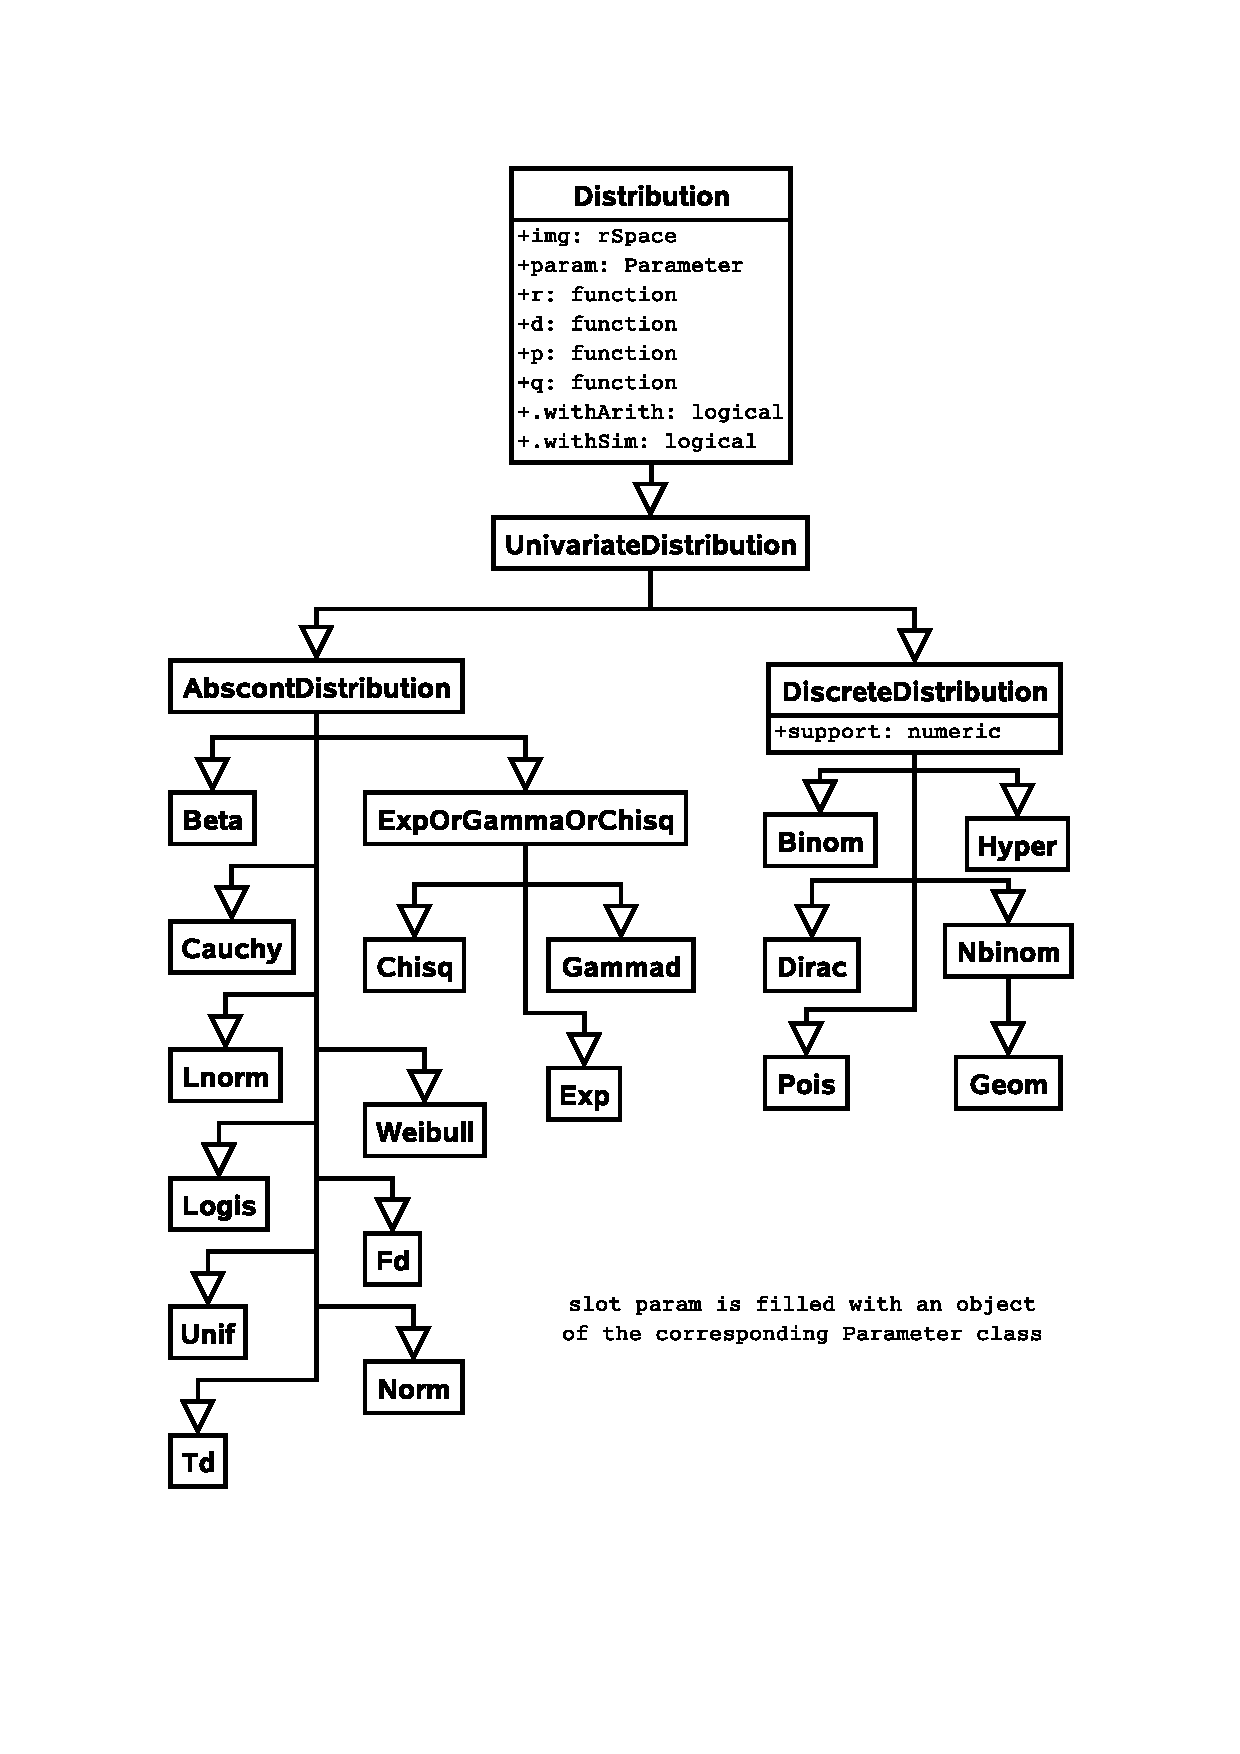
\includegraphics[viewport=0 0 500 700,width=9cm]{distribution.pdf}%
    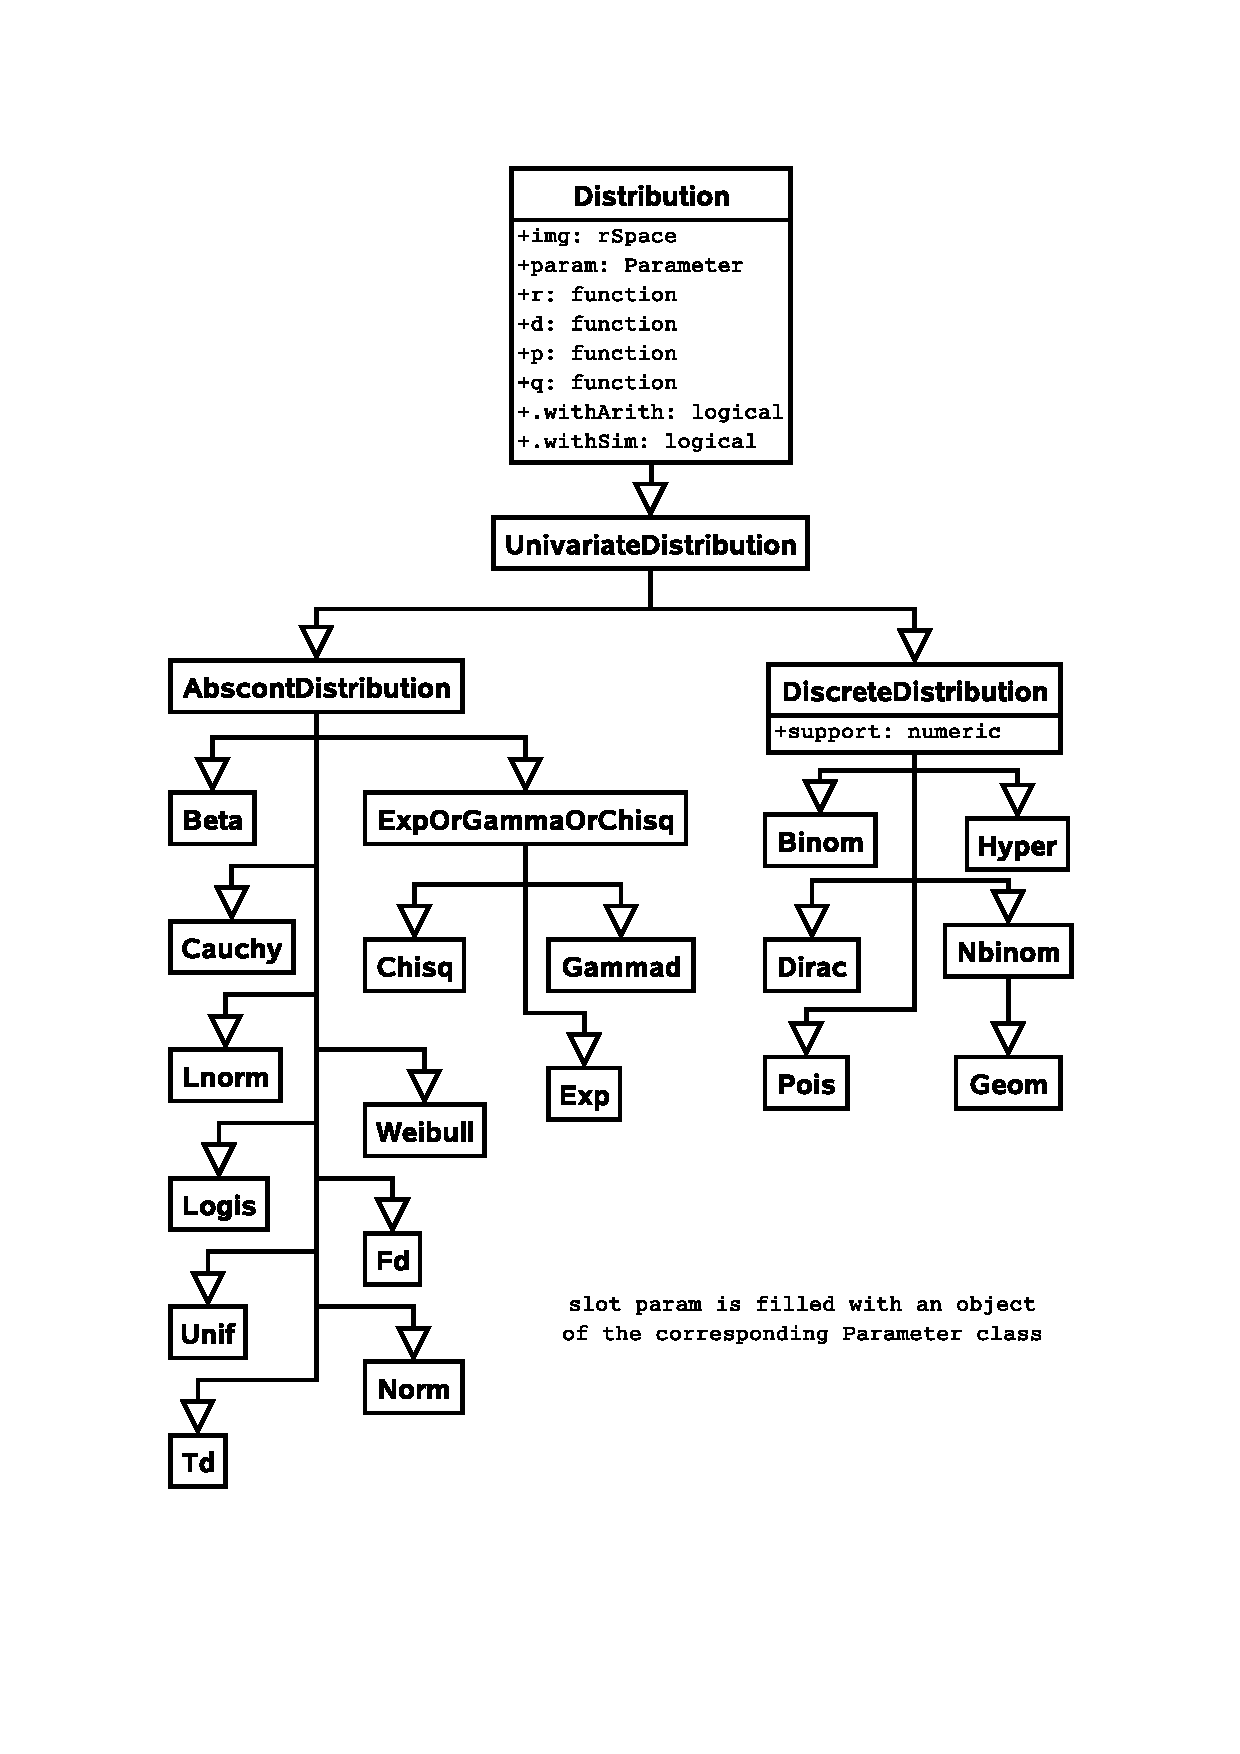
\includegraphics[viewport=130 150 500 750,width=9cm]{distribution.pdf}%
    \caption{\label{fig1c}{\footnotesize Inheritance relations and slots of the
    corresponding \mbox{(sub-)}classes for \code{Distribution} where we do not
    repeat inherited slots
    }}
  \end{center}
\vspace{-4ex}
\end{figure}
\else
\begin{figure}[htb]\label{fig1}
  \begin{center}
    \includegraphics[viewport=130 150 500 730,width=7.5cm]{distribution.ps}%
    \caption{\label{fig1c}{\footnotesize Inheritance relations and slots of the
    corresponding \mbox{(sub-)}classes for \code{Distribution} where we do not
    repeat inherited slots
    }}
  \end{center}
\vspace{-1ex}
\end{figure}
\fi

The most powerful use of our package probably consists in operations to
automatically generate new slots \code{r}, \code{d}, \code{p}, and \code{q}
---induced by mathematical transformations. This is discussed in some detail in
subsection~{\ref{methods}}.

\subsubsection{Classes for Mixture Distributions}

\paragraph{Lists of distributions}

As a first step, we allow distributions to be gathered in lists, giving
classes \code{DistrList} and \code{UnivarDistrList}, where in case of the latter,
all elements must be univariate distributions. For these, the usual indexing
operations with \code{[[.]]} are available. As we will use these lists to
construct more general mixture distributions in some subsequent versions, we
have moved these routines to package \pkg{distr} from version 1.9 on.


\paragraph{Mixing distributions}

To be able to work with distributions which are neither purely absolutely continuous
nor purely discrete, like e.g.\ the distribution of $\min(X,1)$ for
$X\sim{\cal N}(0,1)$, from package version 2.0 on, we support mixtures of
distributions. These are realized as subclasses of class \code{UnivariateDistribution}.
To begin with, we introduce a class \code{UnivarMixingDistribution} as subclass of
class \code{UnivariateDistribution} which additionally has two slots \code{MixCoeff}
and \code{MixDistr}. While the former is a numeric vector taking up the mixture
coefficients of the distribution, the latter is an object of class
\code{UnivarDistrList} as described below, taking up the distributions of the
mixture components; as usual, these slots have their respective accessor and
replacement functions. Usually, this mixing distribution will neither have
a Lebesgue density nor be purely discrete, having a counting density. So slot
\code{d} as a rule will be empty. Objects of this class may be generated by
the generating function \code{UnivarMixingDistribution()},  see also
the corresponding help. In addition there is the function \code{flat.mix}
to simplify such an object converting it to an object of class
\code{UnivarLebDecDistribution}; confer subsection~\ref{flat}.
Note that these mixing distributions may be recursive, i.e.\ compoments of
slot \code{MixDistr} may again
be of class \code{UnivarMixingDistribution}.
\begin{Schunk}
\begin{Sinput}
> library(distr)
> M1 <- UnivarMixingDistribution(Norm(), Pois(lambda=1), Norm(),
+       withSimplify = FALSE)
> M2 <- UnivarMixingDistribution(M1, Norm(), M1, Norm(), withSimplify = FALSE)
> M2
\end{Sinput}
\begin{Soutput}
An object of class "UnivarMixingDistribution"
 ---------------------------------------------
 It consists of  4 components
 Components:
 [[1]]An object of class "UnivarMixingDistribution"
       :---------------------------------------------
       :It consists of  3 components
       :Components:
       :[[1]]Distribution Object of Class: Norm
       :      :mean: 0
       :      :sd: 1
       :[[2]]Distribution Object of Class: Pois
       :      :lambda: 1
       :[[3]]Distribution Object of Class: Norm
       :      :mean: 0
       :      :sd: 1
       :---------------------------------------------
       :Weights:
       :0.333000       :0.333000       :0.333000       :
 ---------------------------------------------
 [[2]]Distribution Object of Class: Norm
       :mean: 0
       :sd: 1
 [[3]]An object of class "UnivarMixingDistribution"
       :---------------------------------------------
       :It consists of  3 components
       :Components:
       :[[1]]Distribution Object of Class: Norm
       :      :mean: 0
       :      :sd: 1
       :[[2]]Distribution Object of Class: Pois
       :      :lambda: 1
       :[[3]]Distribution Object of Class: Norm
       :      :mean: 0
       :      :sd: 1
       :---------------------------------------------
       :Weights:
       :0.333000       :0.333000       :0.333000       :
 ---------------------------------------------
 [[4]]Distribution Object of Class: Norm
       :mean: 0
       :sd: 1
 ---------------------------------------------
 Weights:
 0.250000 0.250000 0.250000 0.250000
 ---------------------------------------------
\end{Soutput}
\end{Schunk}

\paragraph{Lebesgue Decomposed distributions}

As seen in the above example of $\min(X,1)$, classes \code{DiscreteDistribution}
and \code{Abscontdistribution} are not closed under arithmetic operations. To
have such a closure, from version 2.0 on, we introduce class
\code{UnivarLebDecDistribution}, which realizes a Lebesgue decomposition of a
univariate distribution into a discrete and an absolutely continuous distribution.
Of course, we still cannot cover distributions having a non-trivial continuous
but not absolutely continuous part like the Cantor distribution, but class
\code{UnivarLebDecDistribution} provides a sufficiently general compromise.
Class \code{UnivarLebDecDistribution} is a subclass of class
\code{UnivarMixingDistribution}, where in addition we assume that both slots
\code{MixCoeff} and \code{MixDistr} are of length 2, and that the first component
of slot  \code{MixDistr} is of class \code{AbscontDistribution} while the second
is of class \code{DiscreteDistribution}. For this class there are particular
accessors \code{acWeight}, \code{discreteWeight} for the respective weights and
\code{acPart}, \code{discretePart} for the respective distributions. Again there
is a generating function \code{UnivarMixingDistribution()}.
In addition there is the function \code{flat.LCD}
to simplify such an object converting it to an object of class
\code{UnivarLebDecDistribution}; confer subsection~\ref{flat}.%
Classes \code{AbscontDistribution}, \code{DiscreteDistribution} and
\code{UnivarLebDecDistribution}  are grouped to a virtual class
(more specifically a class union)
\code{AcDcLcDistribution}.

\subsubsection{Classes for multivariate distributions and for conditional
distributions}

In \pkg{distrEx}, we provide the following classes for handling multivariate
distributions:


\paragraph{Multivariate distribution classes}

Multivariate distributions are much more complicated than univariate ones,
which is why but a few exceptional ones have already been implemented to R in
packages like \pkg{multnorm}. In particular it is not so clear what a slot
\code{q} should mean and, in higher dimensions slot \code{p}, and possibly also
slot \code{d} may become awkward. So, for multivariate distributions, realized
as class \code{MultivariateDistribution}, we only insist on slot \code{r}, while
the other functional slots may be left void.

The easiest case is the case of a discrete multivariate distribution with finite
support which is implemented as class \code{DiscreteMVDistribution}.

\paragraph{Conditional distribution classes}

Also arising in multivariate settings only are conditional distributions. In our
approach, we realize factorized, conditional distributions where the
(factorized) condition is in fact treated as an additional parameter to the
distribution. The condition is realized as an object of class \code{Condition},
which is a slot of corresponding classes \code{UnivariateCondDistribution}.
This latter is the mother class to classes
\code{AbscontCondDistribution} and \code{DiscreteCondDistribution}.
The most important application of these classes so far is regression, where
the distribution of the observation given the covariates is just realized as
a \code{UnivariateCondDistribution}.

\subsubsection{Parameter classes}
%
As most distributions come with a parameter which often is of own interest, we
endow the corresponding slots of a distribution class with an own parameter
class, which allows for some checking like ``Is the parameter \code{lambda} of
an exponential distribution non-negative?'',
``Is the parameter \code{size} of a binomial a positive integer?''\\
Consequently, we have a method \code{liesIn} that may answer such questions by a
\code{TRUE}/\code{FALSE} statement. Schematically, the inheritance relations of
class \code{Parameter} as well as the slots of the corresponding
\mbox{(sub-)}classes may be read off in figure~\ref{fig4c} where we do not
repeat inherited slots.
%
\ifpdf
\begin{figure}[!ht]\label{fig4}
  \begin{center}
% 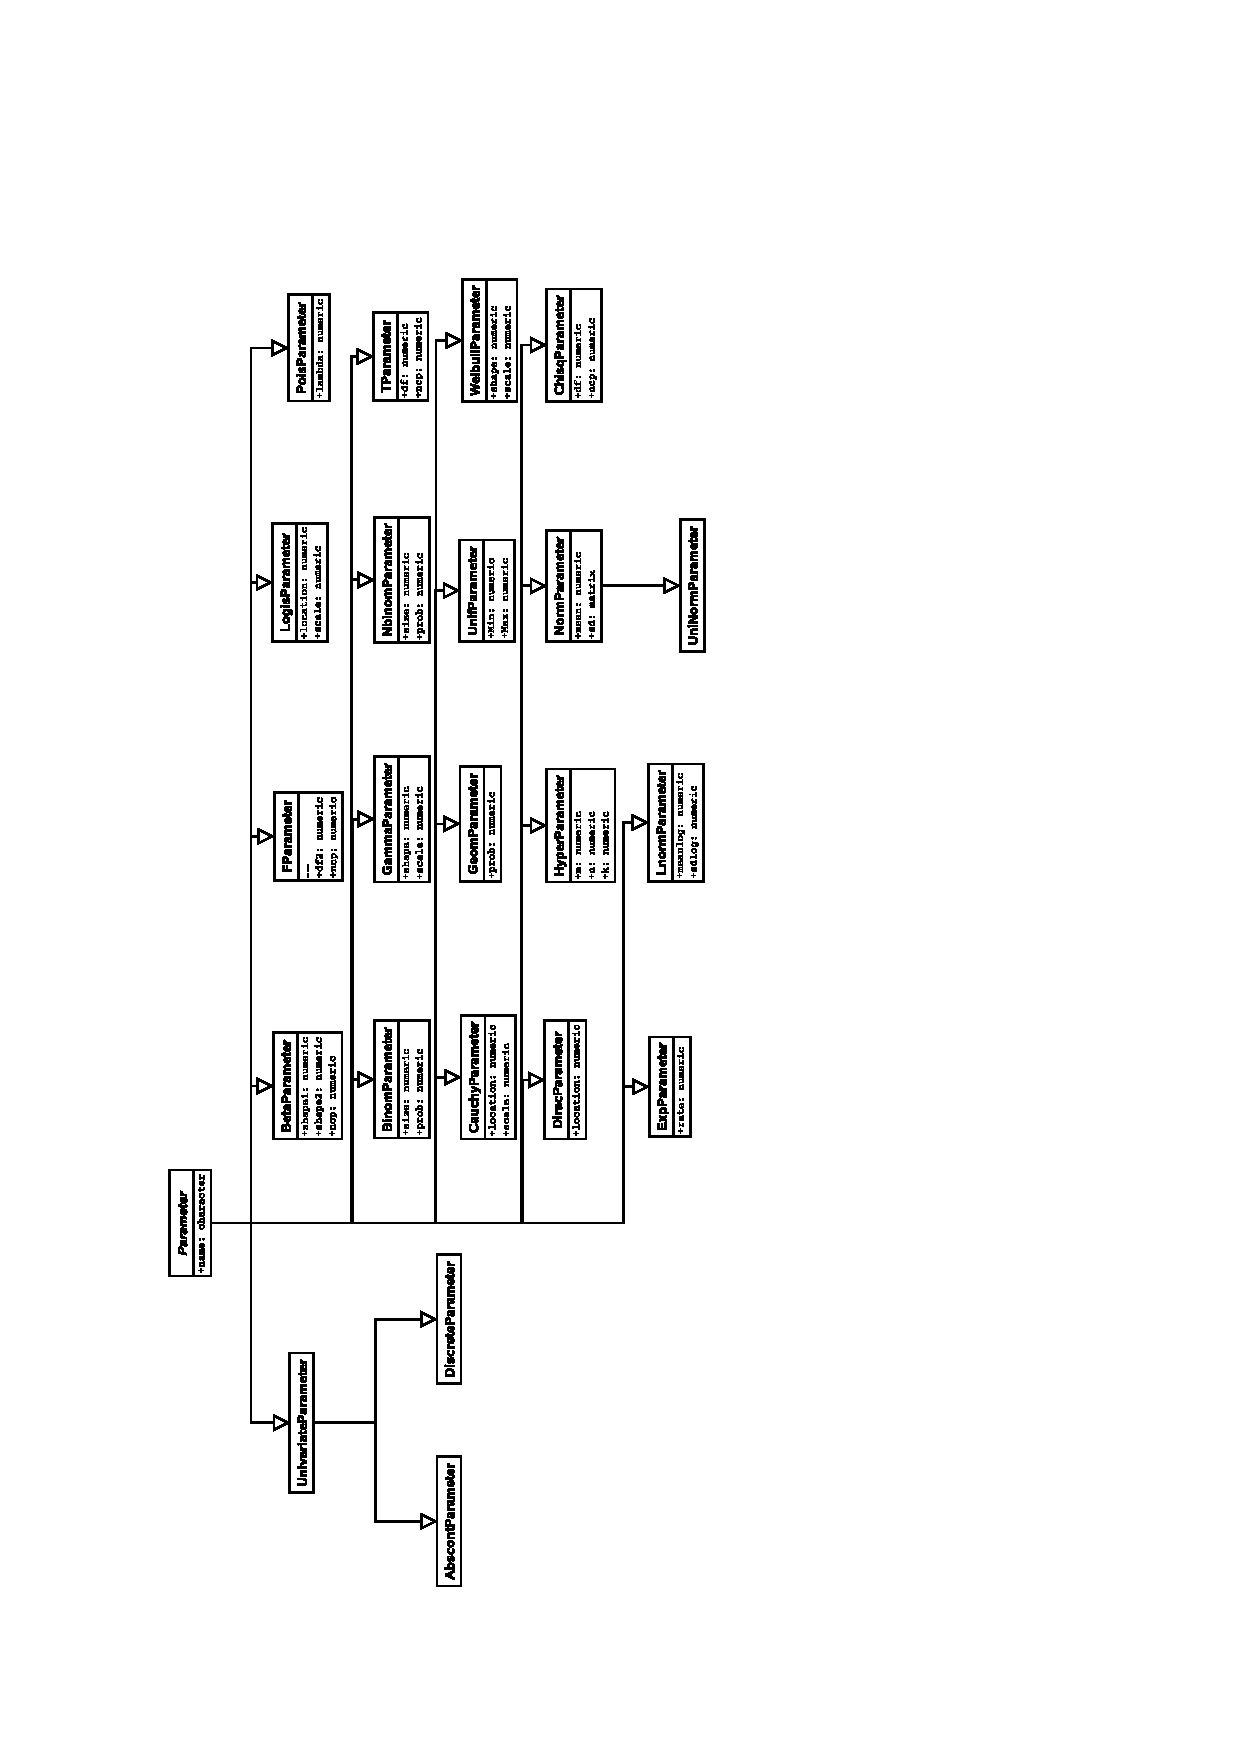
\includegraphics[viewport=30 10 540 390,height=11cm,width=12cm]{parameter.pdf}
% [viewport=30 10 540 390,width=12.cm]
  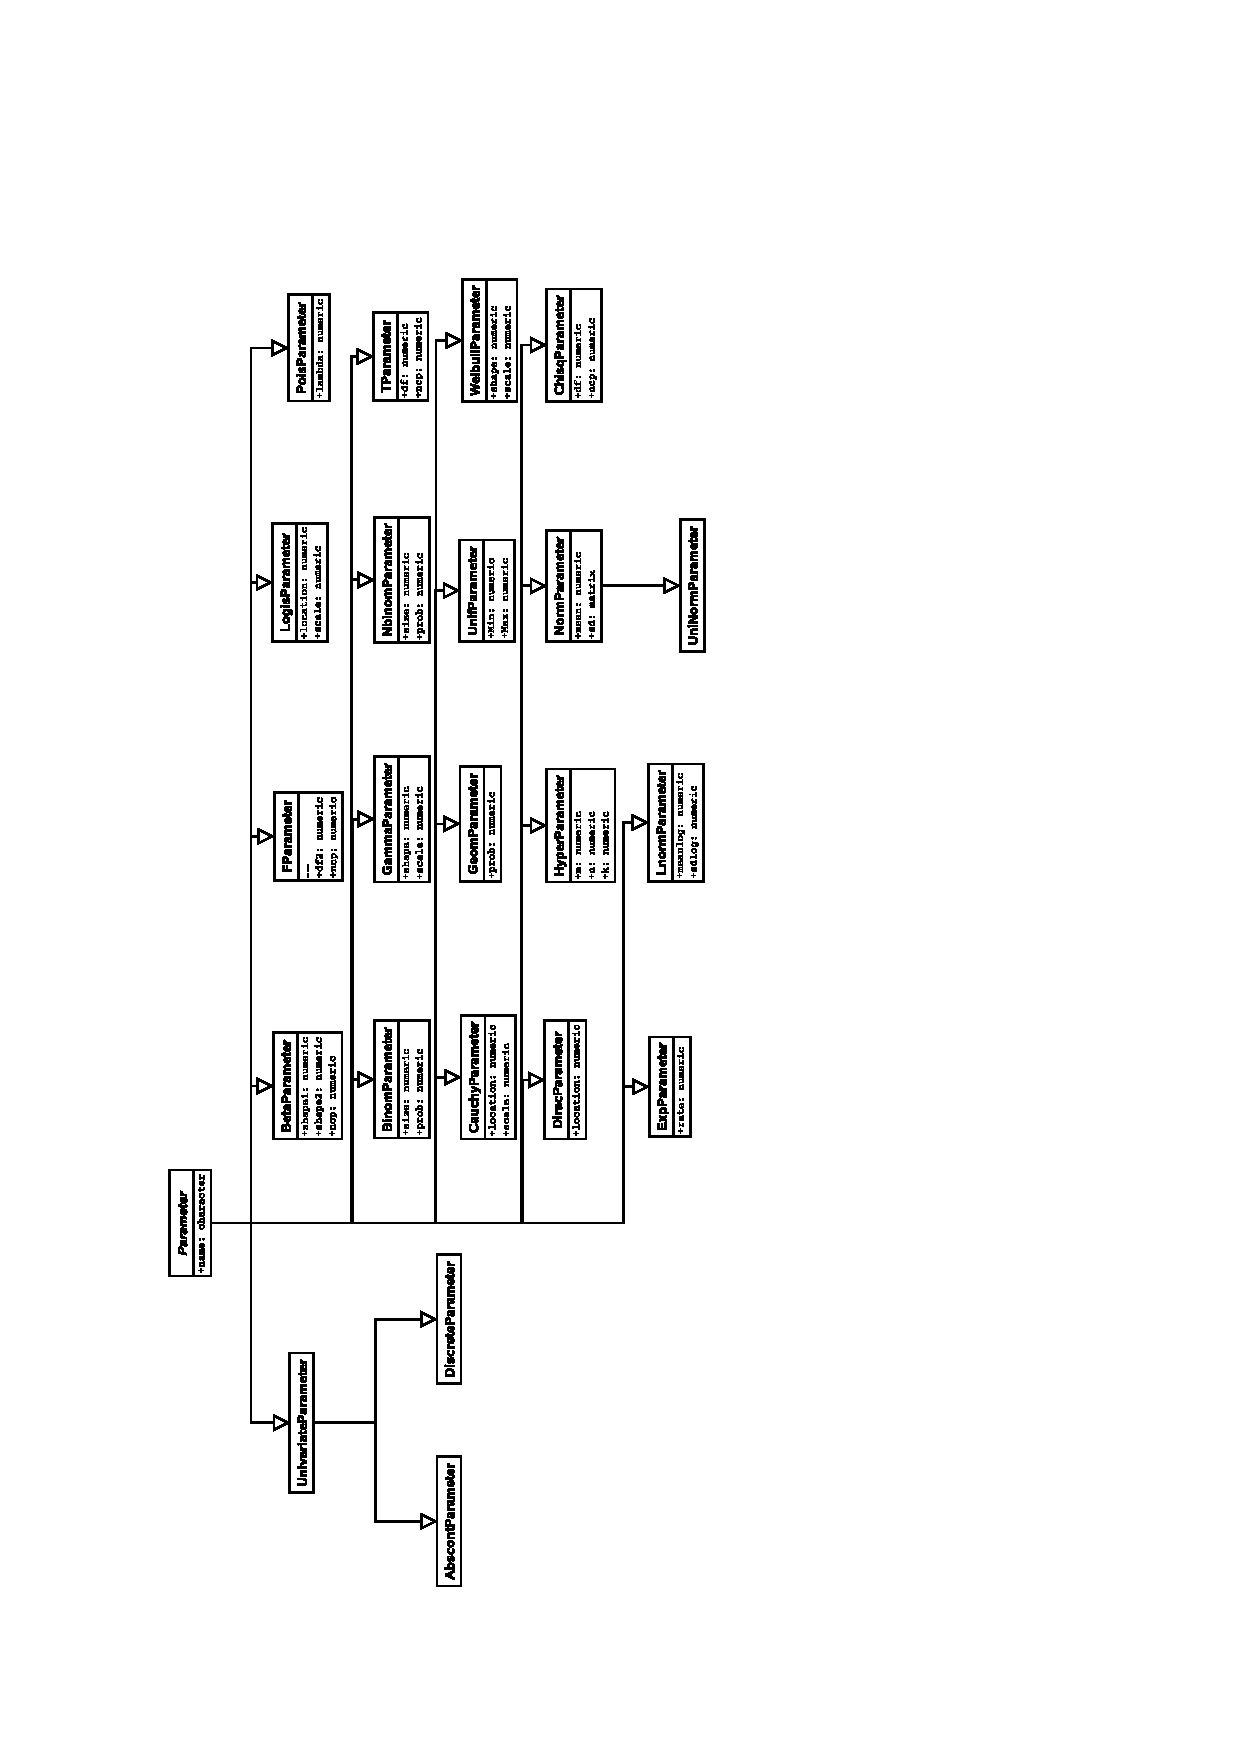
\includegraphics[viewport=30 80 400 690,height=15cm,width=12cm]{parameter.pdf}
    %[viewport=30 10 540 390,width=12.cm]
    \caption{\label{fig4c}{\footnotesize Inheritance relations and slots of the
     corresponding \mbox{(sub-)}classes for \code{Parameter}
    }}
  \end{center}
\end{figure}
\else
\begin{figure}[htb]\label{fig4}
  \begin{center}
    \includegraphics[viewport=80 120 340 600,height=12.8cm,width=9.0cm,
                     angle=-90]{parameter.ps}%
    \caption{\label{fig4c}{\footnotesize Inheritance relations and slots of the
              corresponding \mbox{(sub-)}classes
    for \code{Parameter}
    }}
  \end{center}
\end{figure}
\fi
%
The most important set to be used as parameter domain/sample space
 (\code{rSpace}) will be an Euclidean space. So \code{rSpace} and
 \code{EuclideanSpace} are also implemented as classes,
 the structure of which may be read off in figure~\ref{fig5c}.
\begin{figure}[htb]\label{fig5}
  \begin{center}
    \ifpdf
    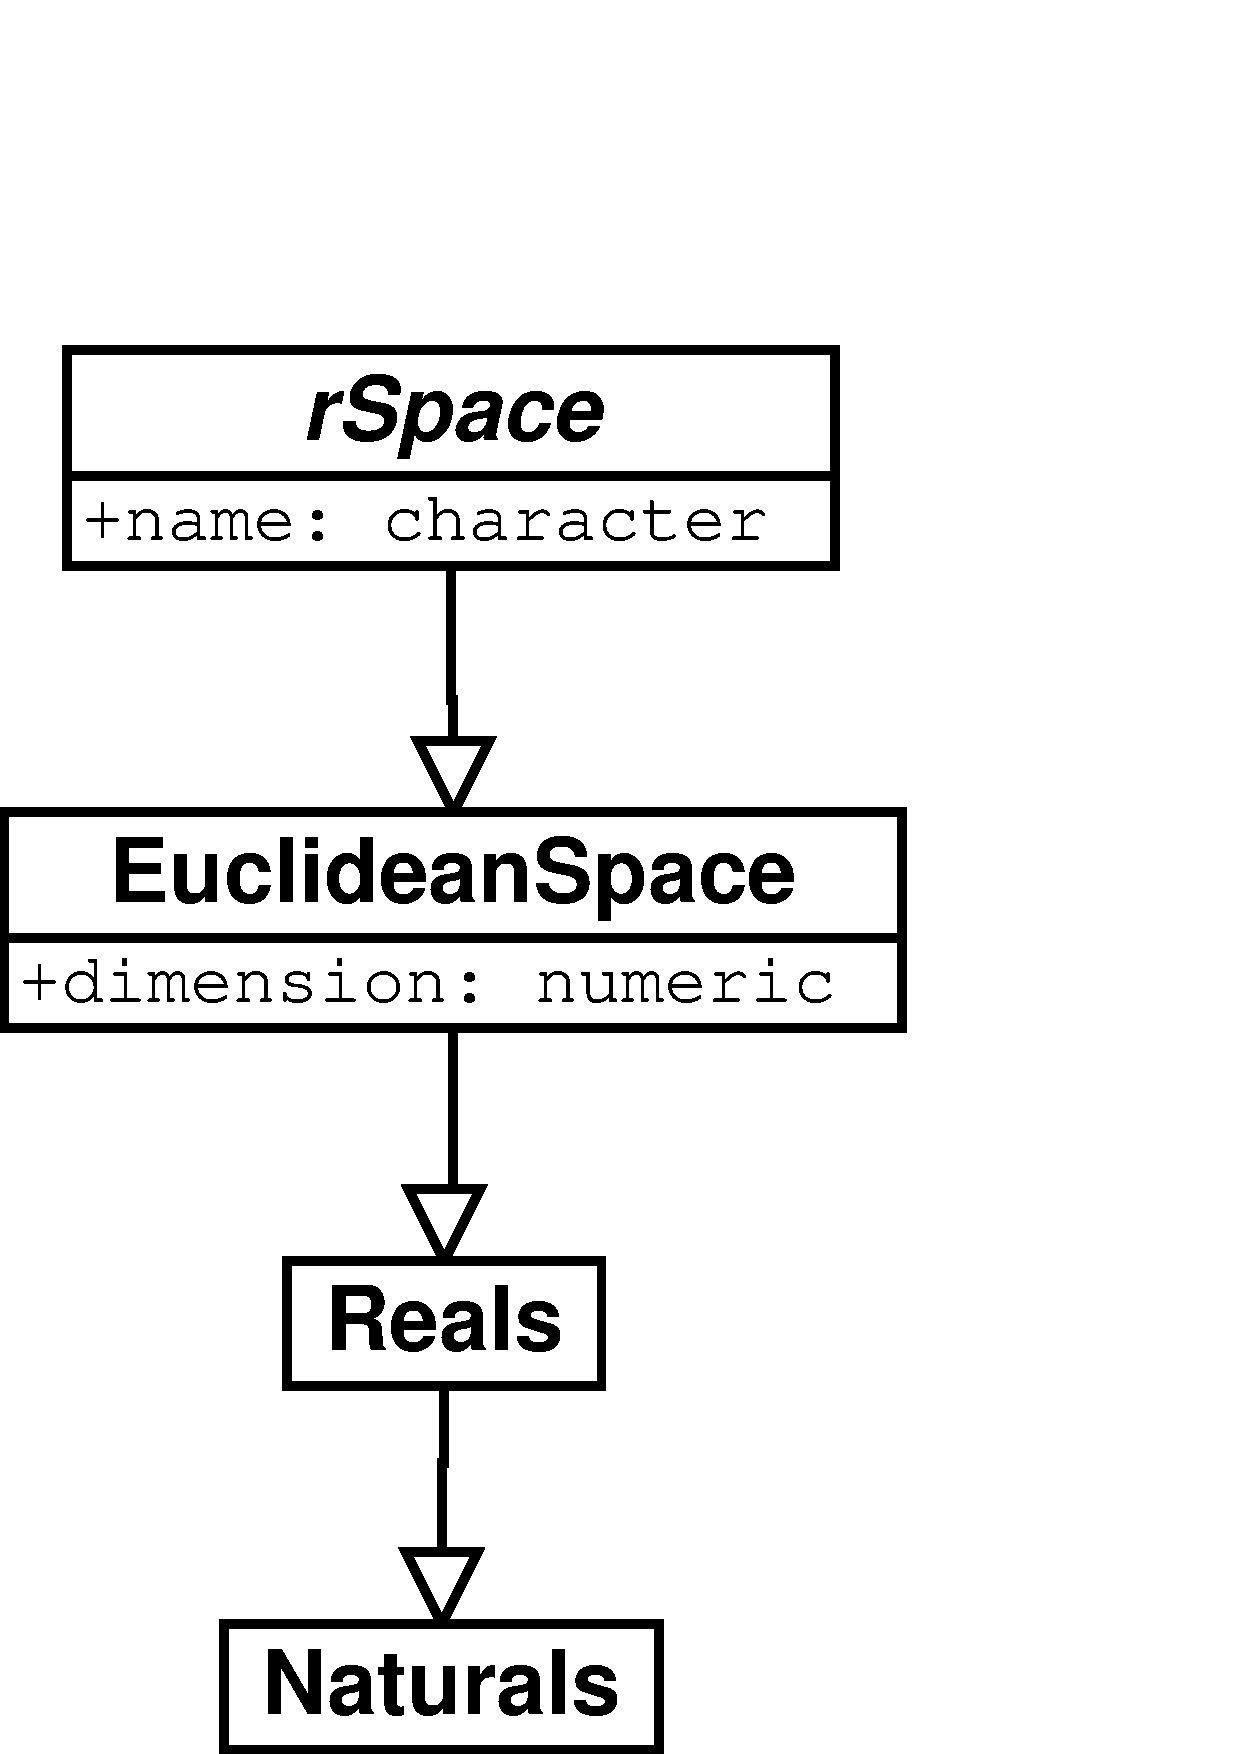
\includegraphics[%viewport=0 30 600 600,
    width=3.9cm]{rspace.pdf}
    \else
    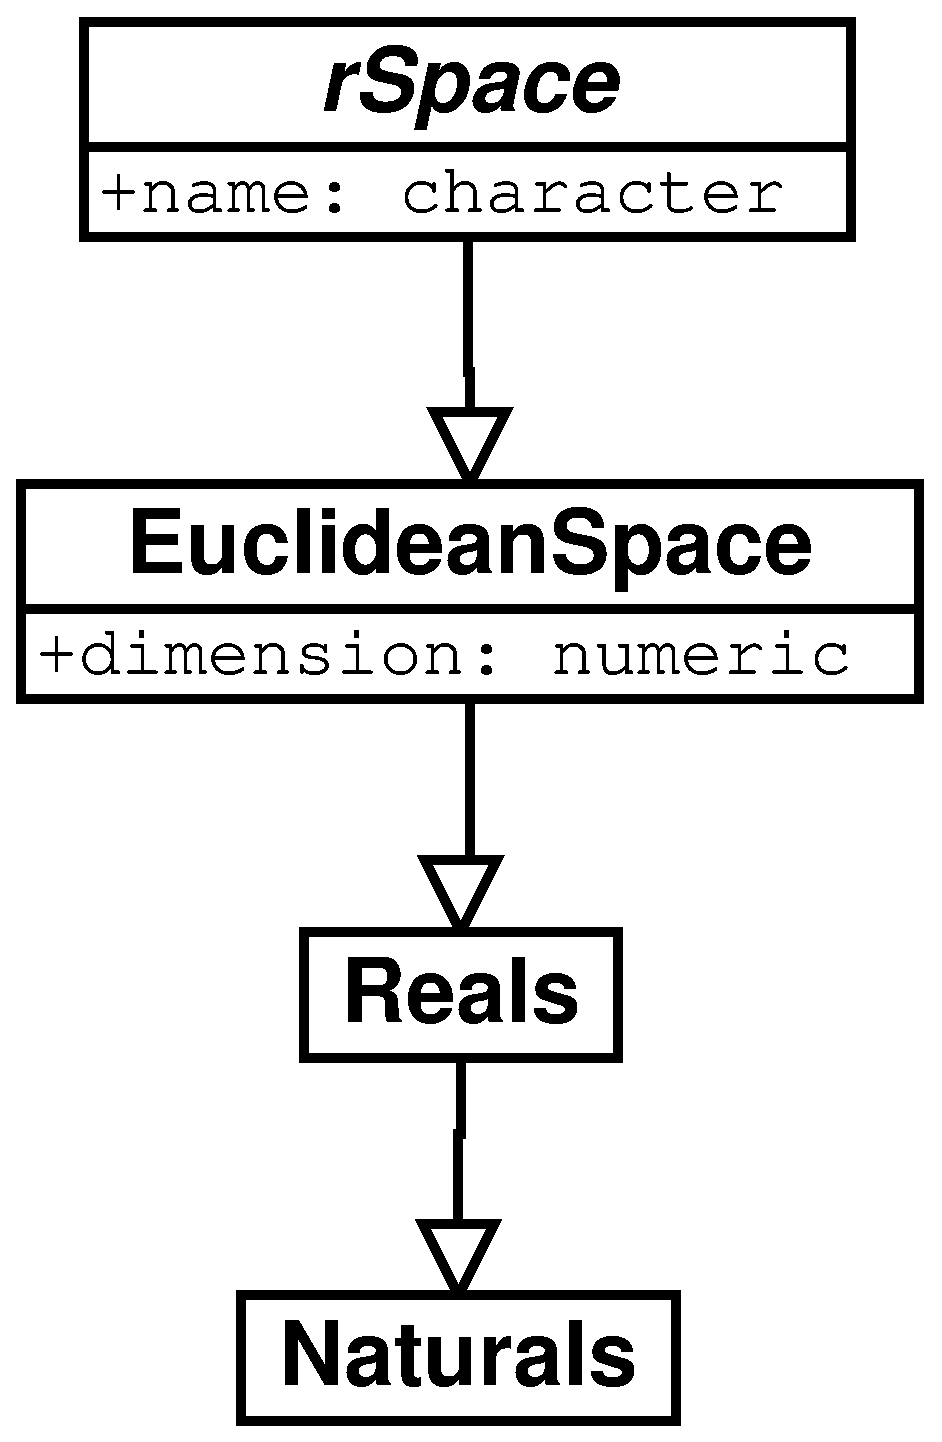
\includegraphics[width=3.7cm]{rspace.ps}%
    \fi
    \caption{\label{fig5c}{\footnotesize Inheritance relations and slots of the
    corresponding \mbox{(sub-)}classes
    for \code{rSpace}
    }}
  \end{center}
\end{figure}

From version 1.9 on, we also have a subclass \code{Lattice}, which is still
lacking in the preceding figure. It has slots \code{pivot} (of class
"numeric"), \code{width} (of class "numeric" but tested against ``{\tt ==0}'')
and  \code{Length} (of class "numeric" but tested to be an integer
``{\tt >0}'' or {\tt Inf}).
All slots may be inspected/modified by the usual accessor/replacement functions.

\subsection{Simulation classes}
From version 1.6 on, the classes and methods of this subsection are available in
package  \pkg{distrSim}.

The aim of simulation classes is to gather all relevant information about a
simulation in a correspondingly designed class. To this end we introduce the
class \code{Dataclass} that serves as a common mother class for both "real" and
simulated data.
%
As derived classes we then have a simulation class where we also gather all
information needed to reconstruct any particular simulation.\\
%
%\newline0??????\\
From version 1.8 of this package on, we have changed the
format how data / simulations are stored:
In order to be able to cope with multivariate,
regression  and (later) time series distributions,
we have switched to the common array format
%
{\tt samplesize x obsDim x runs} where {\tt obsDim} is the dimension of the
observations.
%
For saved objects from earlier versions, we provide the functions
\code{isOldVersion} and \code{conv2NewVersion} to check whether the
object was generated by an older version of this package and
to convert such an object to the new format, respectively.
For objects generated from version 1.8 on, you get the package
version of package~\pkg{distrSim}, under which they have been generated
by a call to \code{getVersion()}. \\
%
%??????1\\
 Finally, coming from robust statistics
we also consider situations where the majority of the data stems from an ideal
situation/distribution whereas a minority comes from a contaminating source. To
be able to identify ideal and contaminating observations, we also store this
information in an indicator variable.\\
%
As the actual values of the simulations only play a secondary role, and as the
number of simulated variables can become very large, but still easily
reproducible, it is not worth storing all simulated observations but rather only
the information needed to reproduce the simulation.
This can be done by \code{savedata}.\\
Schematically, the inheritance relations of class \code{Dataclass} as well as
the slots of the corresponding \mbox{(sub-)}classes may be read off in
figure~\ref{fig2c} where we do not  repeat inherited slots.
\begin{figure}[htb]\label{fig2}
  \begin{center}
    \ifpdf
    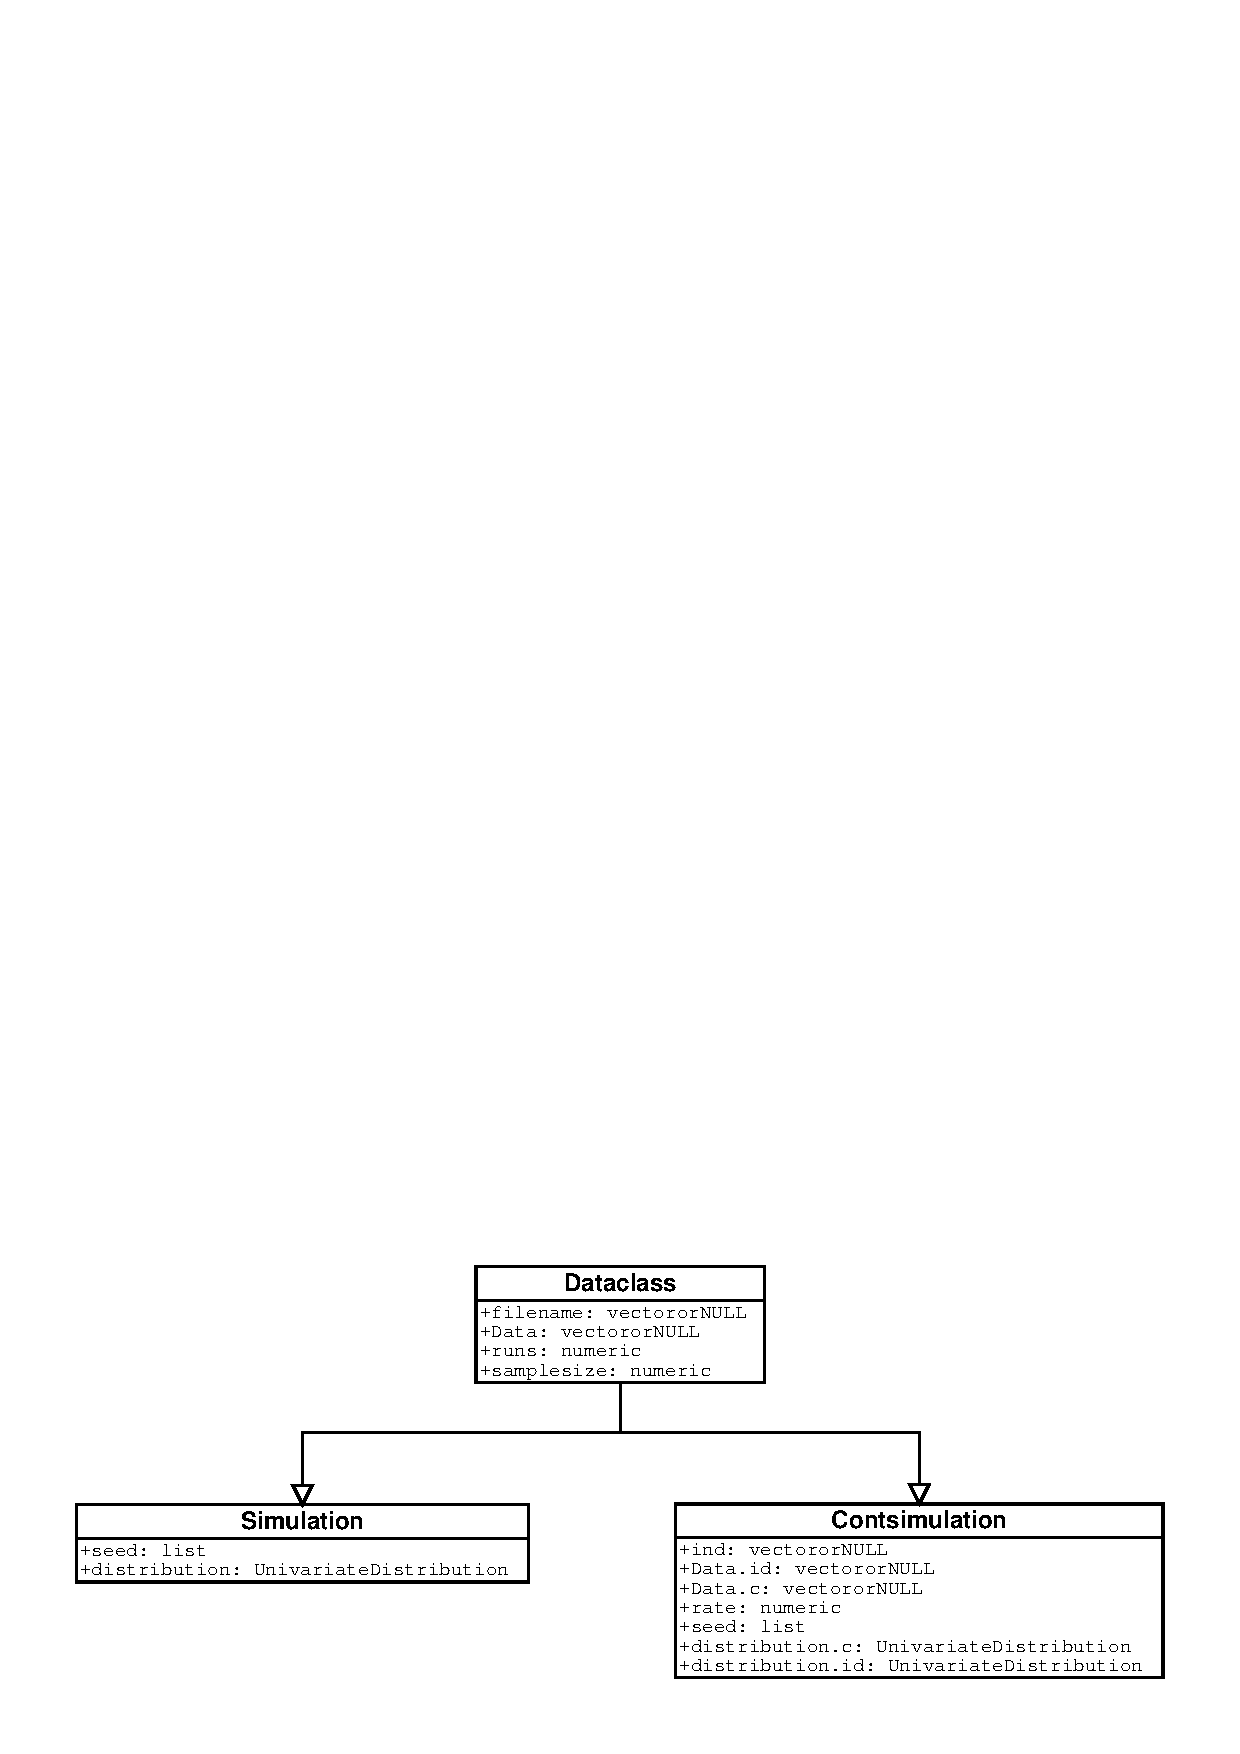
\includegraphics[viewport=120 30 470 250,width=8.5cm]{dataclass.pdf}
    \else
    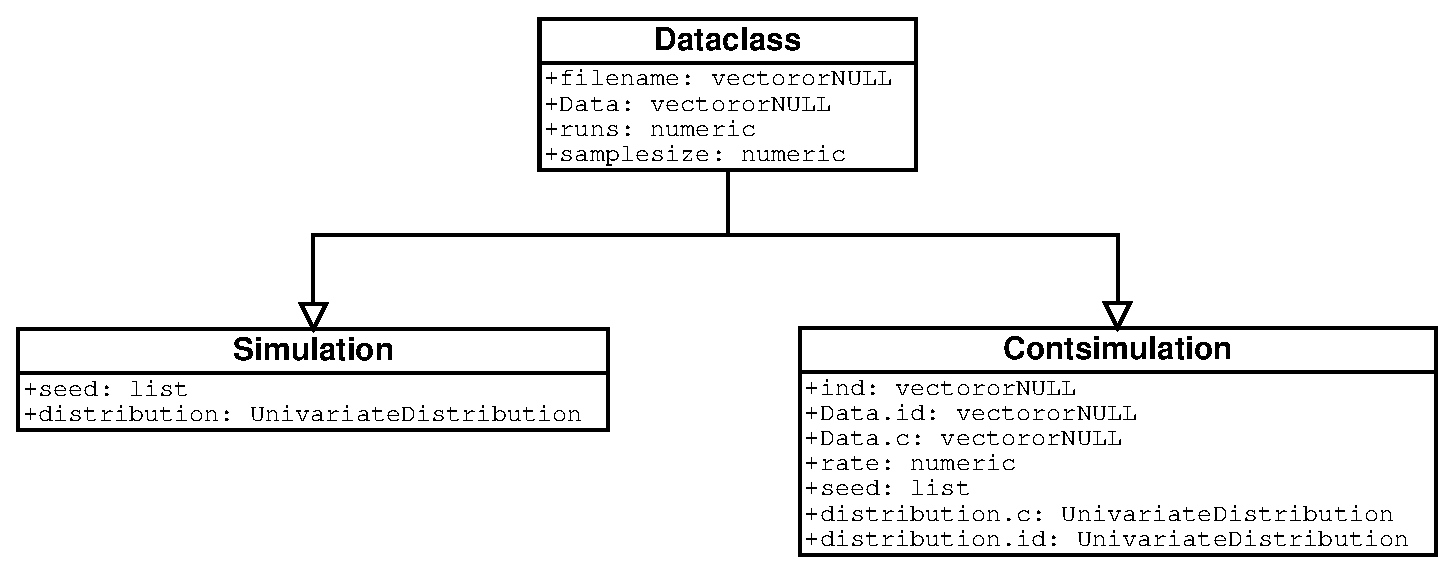
\includegraphics[width=12.5cm]{dataclass.ps}%
    \fi
    \caption{\label{fig2c}{\footnotesize Inheritance relations and slots of the
    corresponding \mbox{(sub-)}classes
    for \code{Dataclass}
    }}
  \end{center}
\end{figure}
%\newline0??????\\
Also, analogously to  package %s
 \pkg{distr}, %and \pkg{distrEx},
 global options for the output by methods \code{plot} and \code{summary}
are controlled by \code{distrSimoptions()} and \code{getdistrSimoptions()}
\smallskip\\
%??????1\\

\subsection{Evaluation class}
From version 1.6 on, the class and methods of
this subsection are available in package  \pkg{distrTEst}. \\
When investigating properties of a new procedure (e.g. an estimator) by means of
simulations, one typically evaluates this procedure on a large set of simulation
runs and gets a result for each run. These results are typically not available
within seconds, so that it is worth storing them.
To organize all relevant information about these results, we introduce a class
\code{Evaluation} the slots of which is filled by method \code{evaluate} ---see
subsection~\ref{evaluate}. Schematically, the slots of this class may be read
off in figure~\ref{fig3c}.
\begin{figure}[htb]\label{fig3}
  \begin{center}
    \ifpdf
    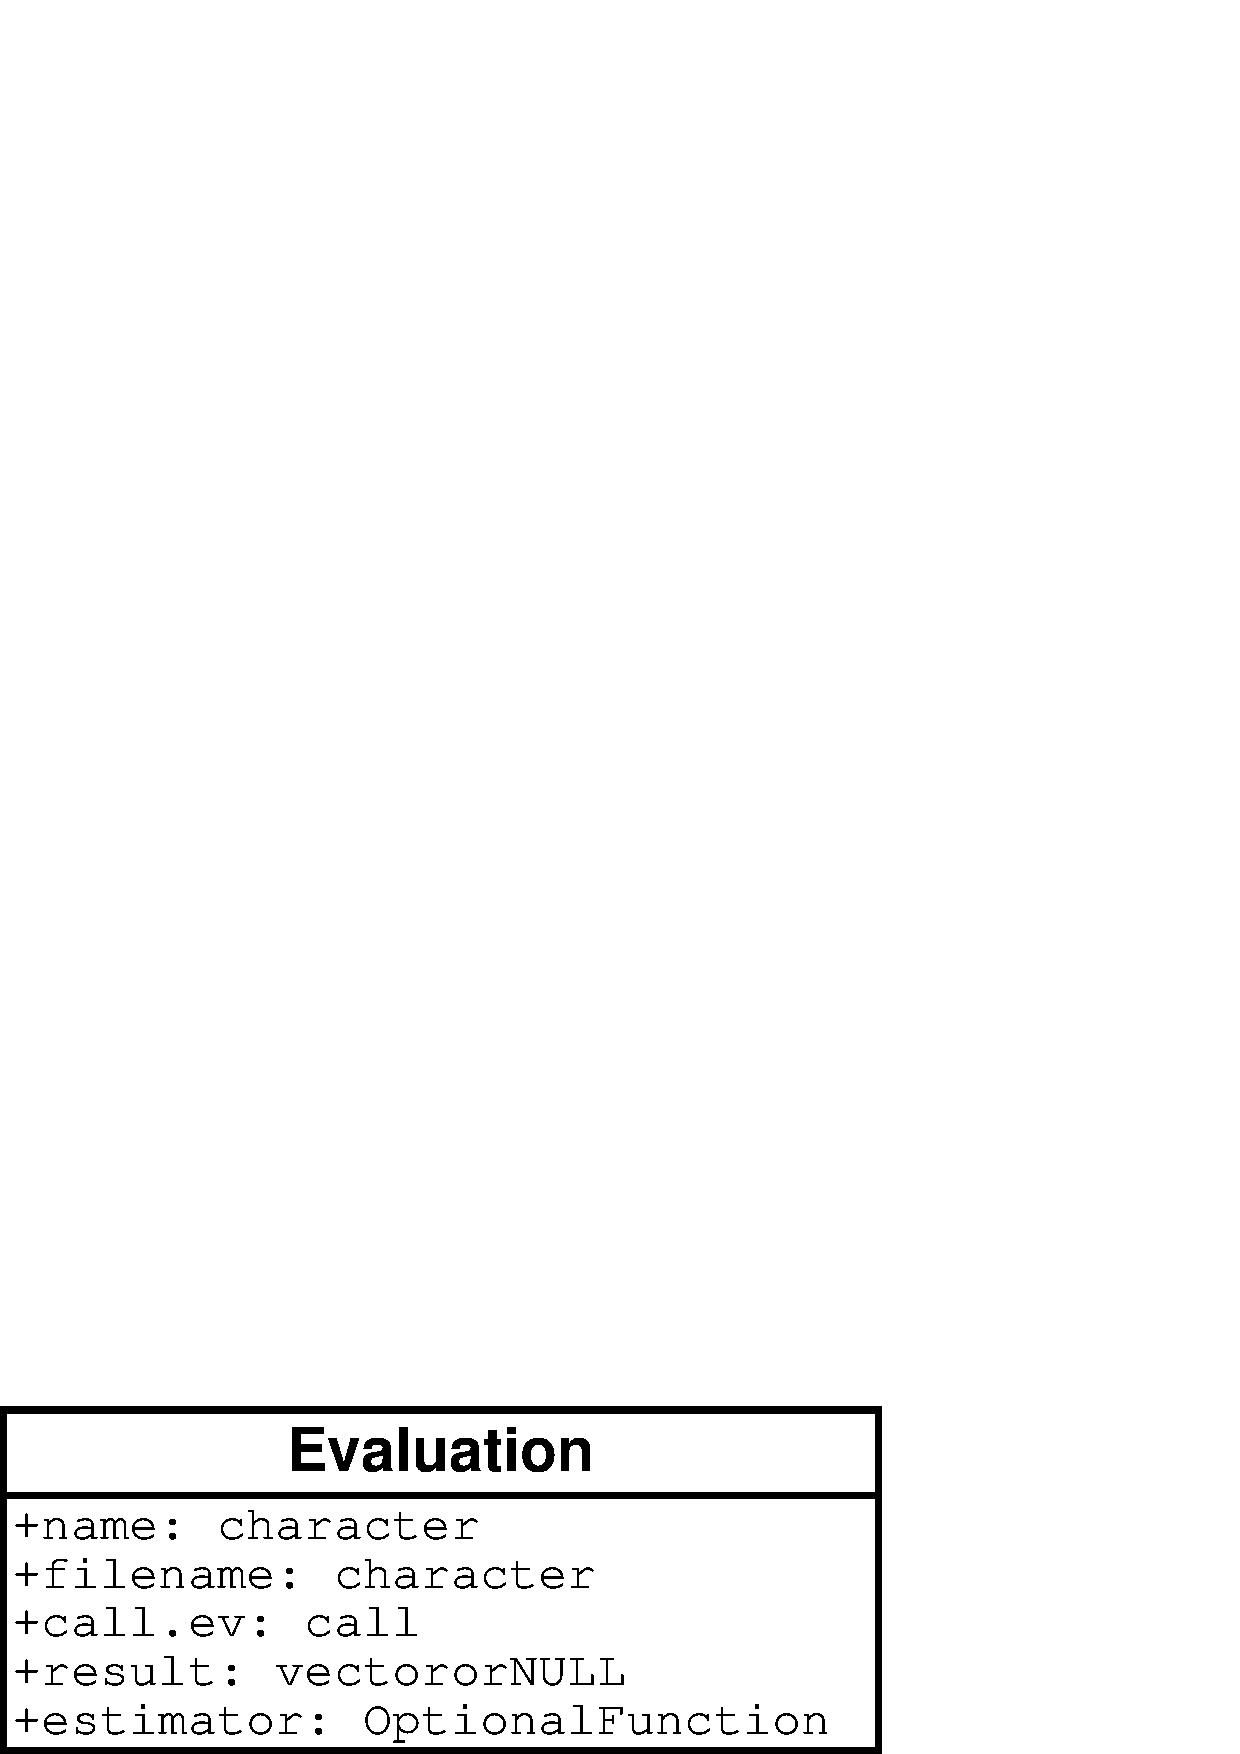
\includegraphics[viewport=60 20 420 200,width=5cm]{evaluation.pdf}
    \else
    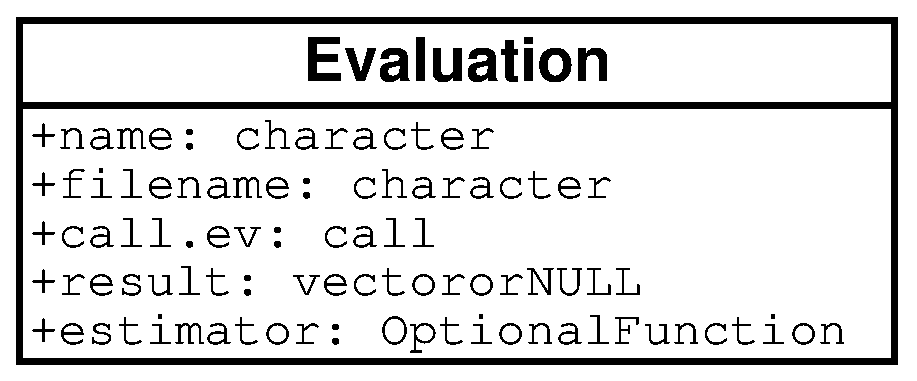
\includegraphics[width=5cm]{evaluation.ps}%
    \fi
    \caption{\label{fig3c}{\footnotesize Slots of class \code{Evaluation}}}
  \end{center}
\end{figure}
%\newline0??????\\
A corresponding \code{savedata} method
saves the object of class \code{Evaluation} in two files in the {\sf R}-working
directory: one using the filename \code{<filename>} also stores the results; the
other one, designed to be ``human readable'', comes as a comment file with
filename \code{<filename>.comment}
only stores the remaining information.
The filename can be specified in the optional argument \code{fileN} to
\code{savedata}; by default it is concatenated from the \code{filename} slot of
the \code{Dataclass} object and \code{<estimatorname>}, which you may either
pass as argument \code{estimatorName} or by default is taken as the {\sf R}-name
of the corresponding {\sf R}-function specified in slot \code{estimator}.

From version 1.8 on, slot \code{result} in class \code{Evaluation} is of class
\code{DataframeorNULL}, i.e.; may be either a data frame or {\tt NULL}, and slot
\code{call.ev} in class \code{Evaluation} is of class "CallorNULL", i.e.; may be
either a call or {\tt NULL}. Also, we want to gather \code{Evaluation} objects
in a particular data structure \code{EvaluationList}
(see below), so we have to be able to check whether all data sets in the
gathered objects coincide.
For this purpose, from this version on, class \code{Evaluation} has an
additional slot \code{Data} of class \code{Dataclass}. In order not to burden
the objects of this class too heavily with uninformative
simulated data, in case of a slot \code{Data} of one of the simulation-type
subclasses of \code{Dataclass},
this \code{Data}  itself has an empty \code{Data}-slot.\\

\subsection{EvaluationList class}
The class and methods of this subsection are available in package
 \pkg{distrTEst}. \\
In order to compare different procedures / estimators for the
same problem, it is natural to gather several \code{Evaluation} objects
with results of the same range (e.g.\ a parameter space) generated on the
same data, i.e.; on the same \code{Dataclass} object. To this end, from
version 1.8 on, we have introduced class \code{EvaluationList}.
Schematically, the slots of this class may be read off in figure~\ref{fig3c1}.
\begin{figure}[htb]\label{fig3-1}
  \begin{center}
    \ifpdf
    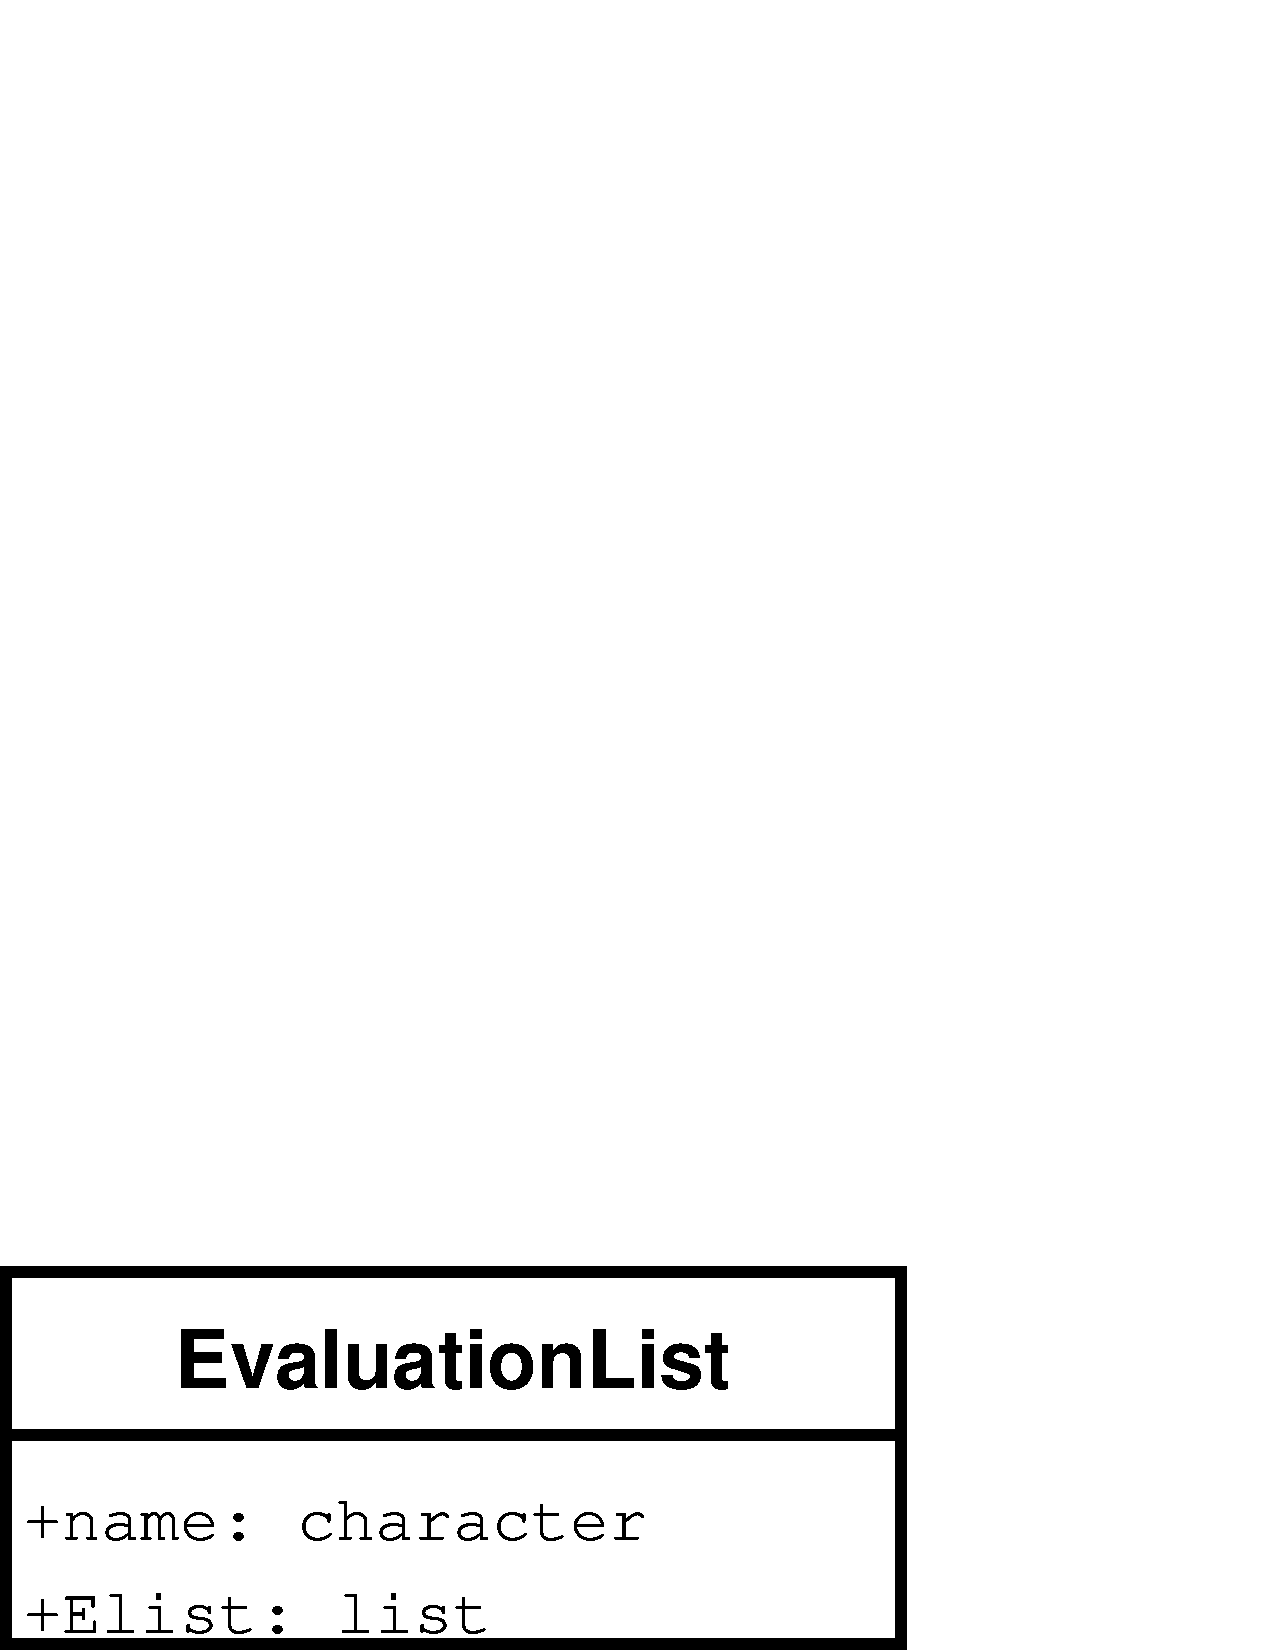
\includegraphics[viewport=0 0 436 185,width=5.5cm]{EvaluationList.pdf}%
    \else
    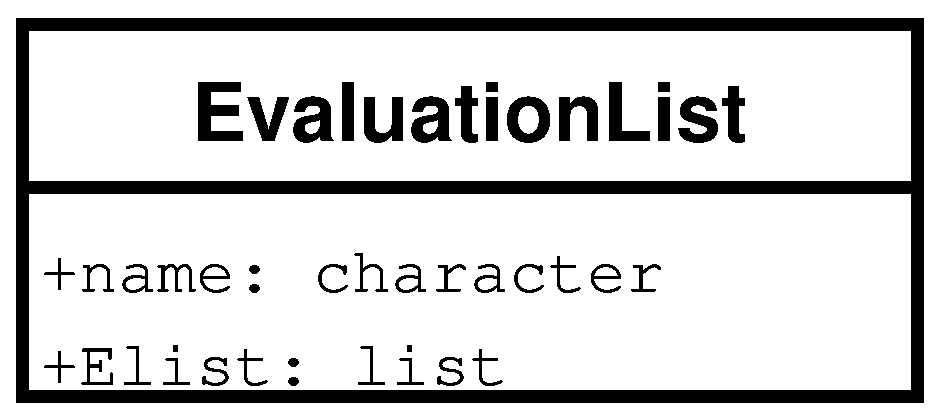
\includegraphics[viewport=0 0 436 185,width=5.5cm]{EvaluationList.ps}%
    \fi
%\parbox{10cm}{TO BE DONE}
    \caption{\label{fig3c1}{\footnotesize Slots of class \code{EvaluationList}}}
  \end{center}
\end{figure}
The common \code{Data} slot of the \code{Evaluation} objects in an
\code{EvaluationList} object may be accessed by the accessor method \code{Data}.
%??????1\\
%
%
\section{Methods}\label{methods}
%
We have made available quite general arithmetical operations to our distribution
objects, generating new image distributions automatically.

\begin{description}
  \item[{\Large \sc Caveat:\/}] {\bf These arithmetics
operate on the corresponding r.v.'s and {\bf not} on the distributions.}
\end{description}
(For the latter, they only would make sense in restricted cases like convex
 combinations).\\

Martin M\"achler pointed out that this might be confusing. So, this warning is
also issued on attaching package \pkg{distr}, and,  by default, again whenever a
\code{Distribution} object, produced by such arithmetics is shown or printed;
this also applies to the last line in
\begin{Schunk}
\begin{Sinput}
>   A1 <- Norm(); A2 <- Unif()
>   A1 + A2
\end{Sinput}
\begin{Soutput}
Distribution Object of Class: AbscontDistribution
\end{Soutput}
\end{Schunk}
\begin{verbatim}
Warning message:
arithmetics on distributions are understood as operations on r.v.'s
see 'distrARITH()'; for switching off this warning see '?distroptions' in:
print(object)
\end{verbatim}
This behaviour will soon be annoying so you may switch it off setting the global
option
\code{WarningArith} to \code{FALSE} (see section~\ref{options}).
%
\subsection{Affine linear transformations}\label{afflin}
%
We have overloaded the operators \code{"+"}, \code{"-"}, \code{"*"}, \code{"/"}
such that affine linear transformations which involve only single univariate
r.v.'s are available;
i.e.\ is expressions like \code{Y=(3*X+5)/4} are permitted for an object
\code{X} of class \code{AbscontDistribution}
or \code{DiscreteDistribution}
(or some subclass), giving again an object \code{Y} of
class \code{AbscontDistribution} or \linebreak[4]\code{DiscreteDistribution}
(in general).
Here the corresponding transformations of the \code{d}, \code{p}, and
\code{q}-functions are done analytically.\\
%
From version 1.9 on, we use subclasses
\code{AffLinAbscontDistribution}, \code{AffLinDiscrete\-Distribution},
\code{AffLinLatticeDistribution} as classes of the return values to enhance
accuracy of functinals like \code{E}, \code{var}, etc.\
in package \pkg{distrEx}. These classes in addition
to their counterparts without prefix ``\code{AffLin}'' have slots \code{a}, \code{b},
and \code{X0}, to capture the fact that an object of this class is distributed
as \code{a * X0 + b}. Also, we introduce a class union \code{AffLinDistribution}
of classes \code{AffLinAbscontDistribution} and
\linebreak[4]\code{AffLinDiscrete\-Distribution}.
Consequently, the result \code{Y} of \code{Y <- a1 * X + b1} for an
object \code{X} of (a subclass of) class \code{AffLinDiscrete\-Distribution}
(if \code{ a != 0}) is of the same class as \code{X} but with slots
\code{Y@a = a1 * X@a}, \code{Y@b = b1 + X@b}, \code{Y@X0 = X@X0}.
In version 2.0, the same principle has been applied to introduce class
\code{AffLinUnivarLebDecDistribution}. All \code{AffLin}-xxx distribution
classes are grouped to a virtual class (more specifically a class union)
\code{AffLinDistribution}.
%
\subsection{Decompositions and Flattening}\label{flat}
%
One of the issues when programming the distribution of the multiplication of
independent random variables is that we have to treat positive and negative
part (and, if nontrivial, point mass to $0$) separately. To this end, from
version 2.0 on, there are methods \code{decomposePM} to decompose a
discrete, an absolutely continuous or a Lebesgue decomposed distribution into
its respective parts.
%
\begin{Schunk}
\begin{Sinput}
> decomposePM(Norm())
\end{Sinput}
\begin{Soutput}
$neg
$neg$D
Distribution Object of Class: AbscontDistribution

$neg$w
[1] 0.5


$pos
$pos$D
Distribution Object of Class: AbscontDistribution

$pos$w
[1] 0.5
\end{Soutput}
\begin{Sinput}
>      decomposePM(Binom(2,0.3)-Binom(5,.4))
\end{Sinput}
\begin{Soutput}
$neg
$neg$D
Distribution Object of Class: DiscreteDistribution

$neg$w
[1] 0.758944


$`0`
$`0`$D
Distribution Object of Class: Dirac
 location: 0

$`0`$w
[1] 0.1780704


$pos
$pos$D
Distribution Object of Class: DiscreteDistribution

$pos$w
[1] 0.0629856
\end{Soutput}
\begin{Sinput}
>      decomposePM(UnivarLebDecDistribution(Norm(),Binom(2,0.3)-Binom(5,.4),
+                  acWeight = 0.3))
\end{Sinput}
\begin{Soutput}
$pos
$pos$D
An object of class "UnivarLebDecDistribution"
 --- a Lebesgue decomposed distribution:

    Its discrete part (with weight 0.227000) is a
 Distribution Object of Class: DiscreteDistribution
 This part is accessible with 'discretePart()'.

    Its absolutely continuous part (with weight 0.773000) is a
 Distribution Object of Class: AbscontDistribution
 This part is accessible with 'acPart()'.

$pos$w
discreteWeight
     0.1940899


$neg
$neg$D
An object of class "UnivarLebDecDistribution"
 --- a Lebesgue decomposed distribution:

    Its discrete part (with weight 0.780000) is a
 Distribution Object of Class: DiscreteDistribution
 This part is accessible with 'discretePart()'.

    Its absolutely continuous part (with weight 0.220000) is a
 Distribution Object of Class: AbscontDistribution
 This part is accessible with 'acPart()'.

$neg$w
discreteWeight
     0.6812608


$`0`
$`0`$D
Distribution Object of Class: Dirac
 location: 0

$`0`$w
discreteWeight
     0.1246493
\end{Soutput}
\end{Schunk}

On the other hand, concatenating mathematical operations would easily
yield quite complicated structures. A first thing to do is to look whether
some components carry mass (approximately) 0. \code{simplifyD} uses this to
cancel out such components, and if possible return simpler types; see also
the help to this function.

Also, sometimes one would like to let collapse a whole list of distributions
(as in the \code{MixDistr} of a \code{UnivarMixingDistribution} object)
into a simpler \code{UnivarLebDecDistribution}-class
form. This is what is done in the the functions \code{flat.mix} and
\code{flat.LCD}.

\begin{Schunk}
\begin{Sinput}
> D1 <- Norm()
> D2 <- Pois(1)
> D3 <- Binom(1,.4)
> D4 <- UnivarMixingDistribution(D1,D2,D3, mixCoeff = c(0.4,0.5,0.1),
+       withSimplify = FALSE)
> D <- UnivarMixingDistribution(D1,D4,D1,D2, mixCoeff = c(0.4,0.3,0.1,0.2),
+       withSimplify = FALSE)
> D
\end{Sinput}
\begin{Soutput}
An object of class "UnivarMixingDistribution"
 ---------------------------------------------
 It consists of  4 components
 Components:
 [[1]]Distribution Object of Class: Norm
       :mean: 0
       :sd: 1
 [[2]]An object of class "UnivarMixingDistribution"
       :---------------------------------------------
       :It consists of  3 components
       :Components:
       :[[1]]Distribution Object of Class: Norm
       :      :mean: 0
       :      :sd: 1
       :[[2]]Distribution Object of Class: Pois
       :      :lambda: 1
       :[[3]]Distribution Object of Class: Binom
       :      :size: 1
       :      :prob: 0.4
       :---------------------------------------------
       :Weights:
       :0.400000       :0.500000       :0.100000       :
 ---------------------------------------------
 [[3]]Distribution Object of Class: Norm
       :mean: 0
       :sd: 1
 [[4]]Distribution Object of Class: Pois
       :lambda: 1
 ---------------------------------------------
 Weights:
 0.400000 0.300000 0.100000 0.200000
 ---------------------------------------------
\end{Soutput}
\begin{Sinput}
> D0<-flat.mix(D)
> D0
\end{Sinput}
\begin{Soutput}
An object of class "UnivarLebDecDistribution"
 --- a Lebesgue decomposed distribution:

    Its discrete part (with weight 0.380000) is a
 Distribution Object of Class: DiscreteDistribution
 This part is accessible with 'discretePart(res$value)'.

    Its absolutely continuous part (with weight 0.620000) is a
 Distribution Object of Class: AbscontDistribution
 This part is accessible with 'acPart(res$value)'.
\end{Soutput}
\end{Schunk}

Many arithmetic operations described in the subsequent sections do
this simplification on their return value, according to the global option
\code{SimplifyD}.

\subsection[The group math of unary mathematical operations]{The group
\code{math} of unary mathematical operations}
%
Also the group \code{math} of unary mathematical operations is available for
distribution classes; so
expressions like \code{exp(sin(3*X+5)/4)} are permitted.
%
 The corresponding \code{r} method consists in simply
performing the transformation to the simulated values of \code{X}.
The corresponding (default-) \code{d}, \code{p} and \code{q}-functions are
obtained by simulation, using the technique described in the following
subsection.\\
By means of \code{substitute}, the bodies of the \code{r}, \code{d},
\code{p}, \code{q}-slots of distributions show the parameter values with
which they were generated; in particular,
convolutions and applications of the group \code{math} may be traced in
the \code{r}-slot of a distribution object, compare\newline
\code{r(sin(Norm()) + cos(Unif() * 3 + 2))}.

Initially, it might be irritating that the same ``arithmetic'' expression
evaluated twice in a row gives two different results, compare
\begin{Schunk}
\begin{Sinput}
>   A1 <- Norm(); A2 <- Unif()
>   d(sin(A1 + A2))(0.1)
\end{Sinput}
\begin{Soutput}
[1] 0.3805869
\end{Soutput}
\begin{Sinput}
>   d(sin(A1 + A2))(0.1)
\end{Sinput}
\begin{Soutput}
[1] 0.3859678
\end{Soutput}
\begin{Sinput}
>   sin(A1 + A2)
\end{Sinput}
\begin{Soutput}
Distribution Object of Class: AbscontDistribution
\end{Soutput}
\end{Schunk}
This is due to the fact, that all slots are filled starting from simulations.
To explain this, a warning is issued  by default, whenever a \code{Distribution}
object, filled by such simulations is shown or printed; this also applies to the
last line in the preceding code sniplet. This behaviour may again be switched
off by setting the global option
\code{WarningSim} to \code{FALSE} (see section~\ref{options}).\\

As they are frequently needed, from version 1.9 on, math operations
\code{abs()}, \code{exp()}, and ---if an {\sf R}-version $\ge$ {\tt 2.6.0} is
used--- also \code{log()} are implemented in an analytically exact form,
i.e.; with exact expressions for slots \code{d}, \code{p}, and \code{q}.

%
\subsection{Construction of \code{d}, \code{p}, and \code{q} from \code{r}}
%
In order to facilitate automatic generation of new distributions, in particular
those arising as image distributions under transformations of correspondingly
distributed random variables, we provide ad hoc methods that should be
overloaded by more exact ones wherever possible. As, at least in principle
each of these slots is sufficient for the reconstruction of the other ones,
we follow the following strategy:
\\
\begin{center}
\begin{tabular}{llll|p{10cm}}
\code{d} & \code{p} &  \code{q} & \code{r} & reconstruction\\
\hline
$+$&$+$&$+$&$+$&no reconstruction necessary\\
$+$&$+$&$+$&$-$&\code{r} as \code{q(X)(runif(n))}\\
$+$&$+$&$-$&$+$&\code{q} by numerical inversion from \code{p}\\
$+$&$+$&$-$&$-$&\code{q} again from \code{p} and
                         \code{r} again from slot \code{q}\\
$+$&$-$&$+$&$+$&\code{p} by numerical integration from \code{d}\\
$+$&$-$&$+$&$-$&\code{p} from \code{d}, and \code{r} from  \code{q}\\
$+$&$-$&$-$&$+$&\code{p} from \code{d}, and \code{q} from  \code{p}\\
$+$&$-$&$-$&$-$&\code{p} from \code{d},
\code{q} from \code{p} and \code{r} from  \code{q}\\
$-$&$+$&$+$&$+$&\code{d} by numerical differentiation (with \code{D1ss}
from package \pkg{sfsmisc} from \code{p}\\
$-$&$+$&$+$&$-$&\code{d} from \code{p}, \code{r} from \code{q}\\
$-$&$+$&$-$&$+$&\code{d}, \code{q}  from \code{p}\\
$-$&$+$&$-$&$-$&\code{d}, \code{q}  from \code{p}, \code{r} from \code{q}\\
$-$&$-$&$+$&$+$&\code{p} by numerical inversion from \code{q},
                \code{d} from \code{p}\\
$-$&$-$&$+$&$-$&\code{p}, \code{r} from \code{q}, \code{d} from \code{p}\\
$-$&$-$&$-$&$+$& use \code{RtoDPQ}\\
$-$&$-$&$-$&$-$&not allowed\\
\end{tabular}\\
\end{center}
More specifically, by means of the function
\code{RtoDPQ} we first generate $10^{\footnotesize\tt RtoDPQ.e}$
random numbers where \code{RtoDPQ.e} is a global option of this package and is
discussed in section~{\ref{options}}. %
A density estimator is evaluated along this sample, the distribution function is
estimated by the empirical c.d.f. and, finally, the quantile function is
produced by numerical inversion.
Of course the result is rather crude as it relies on the law of large numbers
only, but this way all transformations within the group \code{math} become
available.
If the input of the transformation is of class \code{UnivarLebDecDistribution},
\code{RtoDPQ} is replaced by \code{RtoDPQ.LC}. In this case, replicated values
are taken as belonging to the discrete part, for which the distribution is
generated according to the corresponding frequencies with the generating
function \code{DiscreteDistribution()}. With the remaining, non replicated
values, the absolutely continuous part is reconstructed just as with \code{RtoDPQ}.

Where laws under transformations can easily be computed exactly ---as for affine
linear transformations--- we replace this procedure by the exactly transformed
\code{d}, \code{p}, \code{q}-methods.
%
\subsection{Convolution}
%
A convolution method for two independent r.v.'s is implemented by means
of explicit calculations for discrete summands, and by means of
DFT/FFT\footnote{Details to be found in \cite{K:R:S:04}} if one of the summands is
absolutely continuous or (from version 1.9 on:) both are lattice distributed
with a common lattice as support.
This method automatically generates the law of the sum of two independent
variables/distributions $X$ and $Y$ of any univariate distributions ---or
in {\tt S4}-jargon: the addition operator \code{"+"} is overloaded for two
objects of class \code{UnivariateDistribution} and corresponding subclasses.
%
\subsection{Further Binary Operators}
%
Having implemented a class for Lebesgue decomposed distributions, we have been
able to realize further binary operators, in particular we have exact
analytical constructions for multiplication, division, exponentiation:
\begin{Schunk}
\begin{Sinput}
>   A1 <- Norm(); A2 <- Unif()
>   A1A2 <- A1*A2
>   plot(A1A2, withSweave = TRUE)
\end{Sinput}
\end{Schunk}
\includegraphics{distr-arith2v1}
\begin{Schunk}
\begin{Sinput}
>   A12 <- 1/(A2 + .3)
>   plot(A12, withSweave = TRUE)
\end{Sinput}
\end{Schunk}
\includegraphics{distr-arith2v2}
\begin{Schunk}
\begin{Sinput}
>   B <- Binom(5,.2)+1
>   A1B <- A1^B
>   plot(A1B, xlim=c(-3,3), withSweave = TRUE)
\end{Sinput}
\end{Schunk}
\includegraphics{distr-arith2v3}
\begin{Schunk}
\begin{Sinput}
>   plot(1.2^A1, withSweave = TRUE)
\end{Sinput}
\end{Schunk}
\includegraphics{distr-arith2V4}
\begin{Schunk}
\begin{Sinput}
>   plot(B^A1, withSweave = TRUE)
\end{Sinput}
\end{Schunk}
\includegraphics{distr-arith2v5}
%
\subsection{Truncation, Pairwise Minimum/Maximum, Huberization}\label{TruncMin}
%
Up to version 2.0, we have had truncation, Huberization and minimum
and maximum of random variables as illustrating demos; in particular
the last three could not be realized in a completely satisfactory manour,
as Lebesgue decomposed distributions had not been available before.
Now these illustrations have moved into the package itself:
\begin{Schunk}
\begin{Sinput}
> H <- Huberize(Norm(),lower=-1,upper=2)
> plot(H, withSweave = TRUE)
\end{Sinput}
\end{Schunk}
\includegraphics{distr-Hub}
\begin{Schunk}
\begin{Sinput}
> T <- Truncate(Norm(),lower=-1,upper=2)
> plot(T, withSweave = TRUE)
\end{Sinput}
\end{Schunk}
\includegraphics{distr-Trun}
\begin{Schunk}
\begin{Sinput}
> M1 <- Maximum(Unif(0,1), Minimum(Unif(0,1), Unif(0,1)))
> plot(M1, withSweave = TRUE)
\end{Sinput}
\end{Schunk}
\includegraphics{distr-Min1}
\begin{Schunk}
\begin{Sinput}
> M2 <- Minimum(Exp(4),4)
> plot(M2, withSweave = TRUE)
\end{Sinput}
\end{Schunk}
\includegraphics{distr-Min2}
\begin{Schunk}
\begin{Sinput}
> M3 <- Minimum(Norm(2,2), Pois(3))
> plot(M3, withSweave = TRUE)
\end{Sinput}
\end{Schunk}
\includegraphics{distr-Min3}
%
\subsection{Overloaded generic functions}
Methods \code{print}, \code{plot}, \code{show} and \code{summary} have been
overloaded for classes \code{Distribution}, \code{Dataclass}, \code{Simulation},
\code{ContSimulation}, as well as \code{Evaluation} and \code{EvaluationList} to
produce ``pretty''  output.
More specifically there are also particular \code{show} methods
for classes \code{UnivarDistrList}, \code{UnivarMixingDistribution} and
\code{UnivarLebDecDistribution}.
%\newline 0??????\\
\code{print}, \code{plot}, \code{show} and \code{summary} have additional,
optional arguments for plotting subsets of the simulations / results:
index vectors for the dimensions, the runs, the observations, and the
evaluations may be passed using arguments \code{obs0},  \code{runs0},
\code{dims0}, \code{eval0}, confer
\code{help("<mthd>-methods",package=<pkg>)} where \code{<mthd>} stands for
\code{plot}, \code{show}, \code{print}, or \code{plot}, and \code{<pkg>} stands
for either \pkg{distrSim} or \pkg{distrTEst}.

For an object of class \code{Distribution},
\code{plot} displays the density/probability function, the c.d.f.\ and the
quantile function of a distribution. Note that all usual parameters of
\code{plot} remain valid. For instance, you may increase the axis annotations
and so on. More important, you may also
override the automatically chosen $x$-region by passing an \code{xlim} argument:
\begin{Schunk}
\begin{Sinput}
>   plot(Cauchy(),withSweave = TRUE)
\end{Sinput}
\end{Schunk}
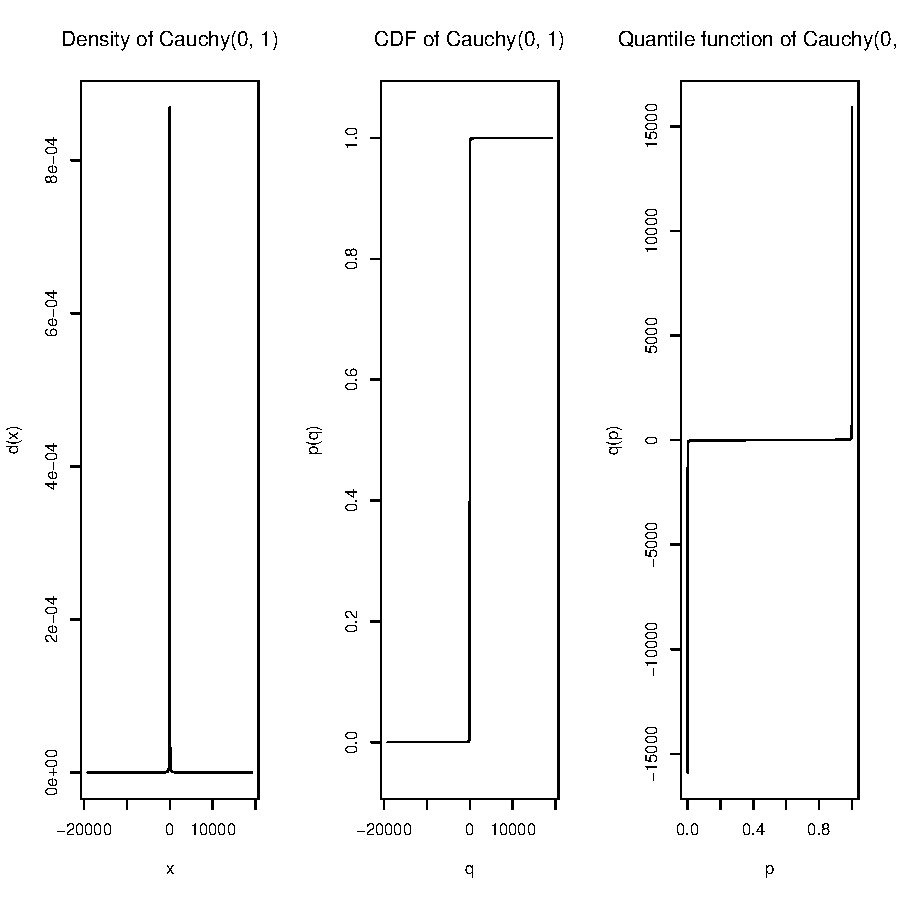
\includegraphics{distr-cauchy1}
\begin{Schunk}
\begin{Sinput}
>   plot(Cauchy(),xlim=c(-4,4),withSweave = TRUE)
\end{Sinput}
\end{Schunk}
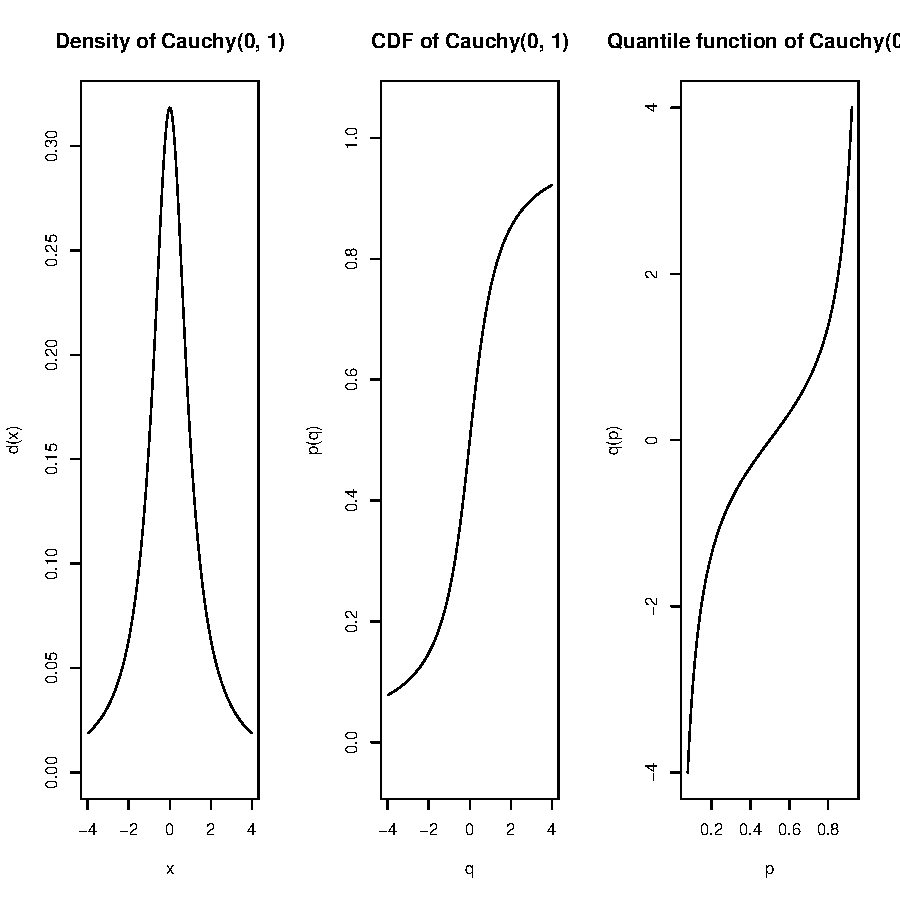
\includegraphics{distr-cauchy2}

Moreover you may control optional main, inner titles and subtitles with
arguments \code{main} / \code{sub} / \code{inner}. To this end there are
preset strings substituted in both expression and character vectors
(where in the following \code{x} denotes the argument
with which \code{plot()} was called)
\begin{itemize}
 \item[\%A] deparsed argument \code{x}
 \item[\%C] class of argument \code{x}
 \item[\%P] comma-separated list of parameter values of slot \code{param} of
            argument \code{x}
 \item[\%Q] comma-separated list of parameter values of slot \code{param} of
            argument \code{x} in parenthesis unless this list is empty; then
            \code{""}
 \item[\%N] comma-separated {\tt <name> = <value>} - list of parameter values of
            slot \code{param} of argument \code{x}
 \item[\%D] time/date at which plot is/was generated
\end{itemize}
As usual you may control title sizes and colors with
\code{cex.main} / \code{cex.inner} / \code{cex.sub} respectively with
\code{col} / \code{col.main} / \code{col.inner} / \code{col.sub}. Additionally
it may be helpful to control top and bottom margins with arguments
\code{bmar}, \code{tmar}. \code{plot()} can also cope with \code{log}-arguments.
We provide different default symbols for unattained [\code{pch.u}] / attained
[\code{pch.a}] one-sided limits, which may be overridden by corresponding
arguments  \code{pch} / \code{pch.a} / \code{pch.u}.

For objects of class \code{AbscontDistribution}, you may set the number of grid
points used by an \code{ngrid} argument; also the ``quantile''-panel
takes care of finite left/right endpoints of support and optionally tries
to identify constancy region of the \code{p}-slot.

For objects of class \code{DiscreteDistributions}, we use \code{stepfun()} from
package \pkg{base} as far as possible and (also for panel ``q'' for
\code{AbscontDistributions}) consequently take over its arguments
\code{do.points}, \code{verticals}, \code{col.points} / \code{col.vert} /
\code{col.hor} and \code{cex.points}.

As examples consider the following 10 plots:


\begin{figure}[p]
\begin{Schunk}
\begin{Sinput}
> plot(Binom(size = 4, prob = 0.3), withSweave = TRUE)
\end{Sinput}
\end{Schunk}

\includegraphics{distr-plotex1}
\end{figure}
\begin{figure}[p]
\begin{Schunk}
\begin{Sinput}
> plot(Binom(size = 4, prob = 0.3), do.points = FALSE, verticals = FALSE,
+      withSweave = TRUE)
\end{Sinput}
\end{Schunk}
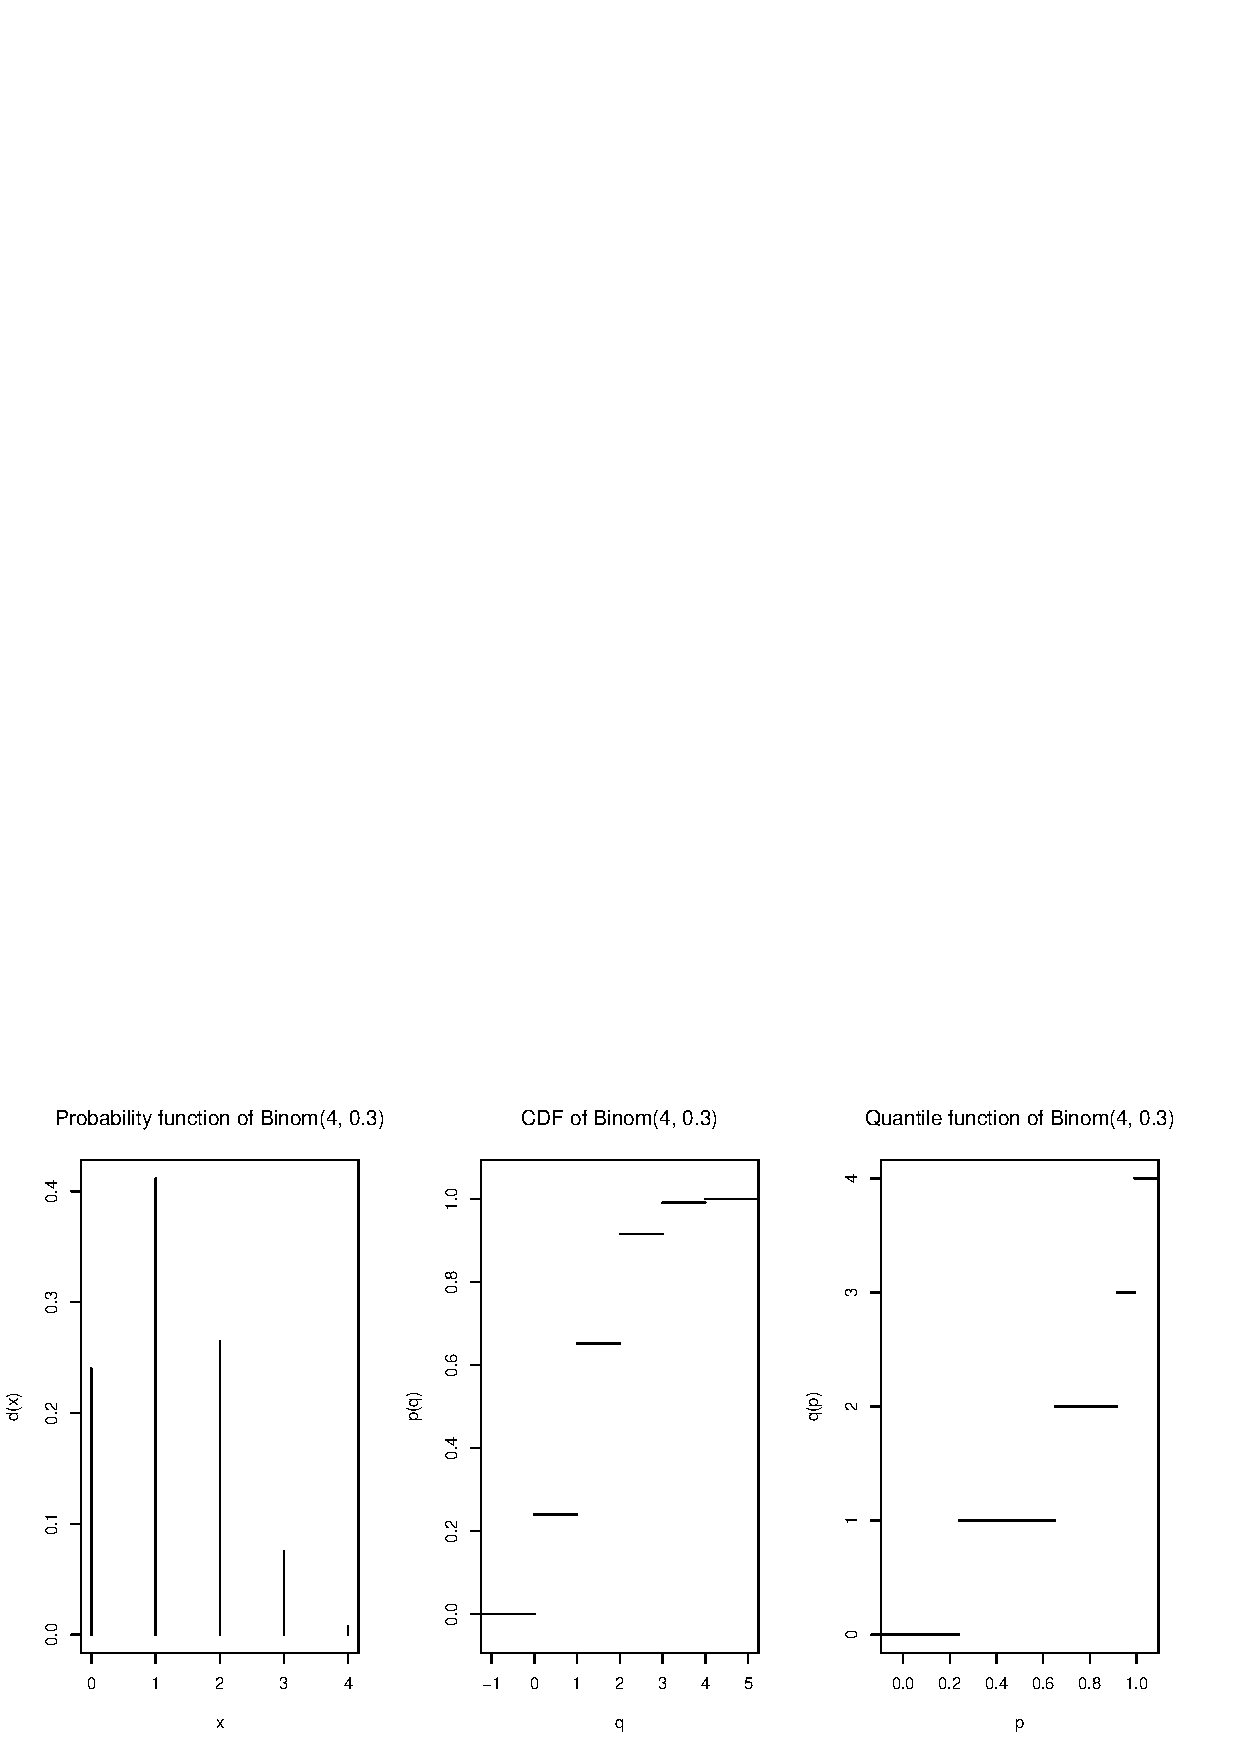
\includegraphics{distr-plotex2}
\end{figure}

\begin{figure}[p]
\begin{Schunk}
\begin{Sinput}
> plot(Binom(size = 4, prob = 0.3), main = TRUE, inner = FALSE, cex.main = 1.6,
+      tmar = 6, withSweave = TRUE)
\end{Sinput}
\end{Schunk}
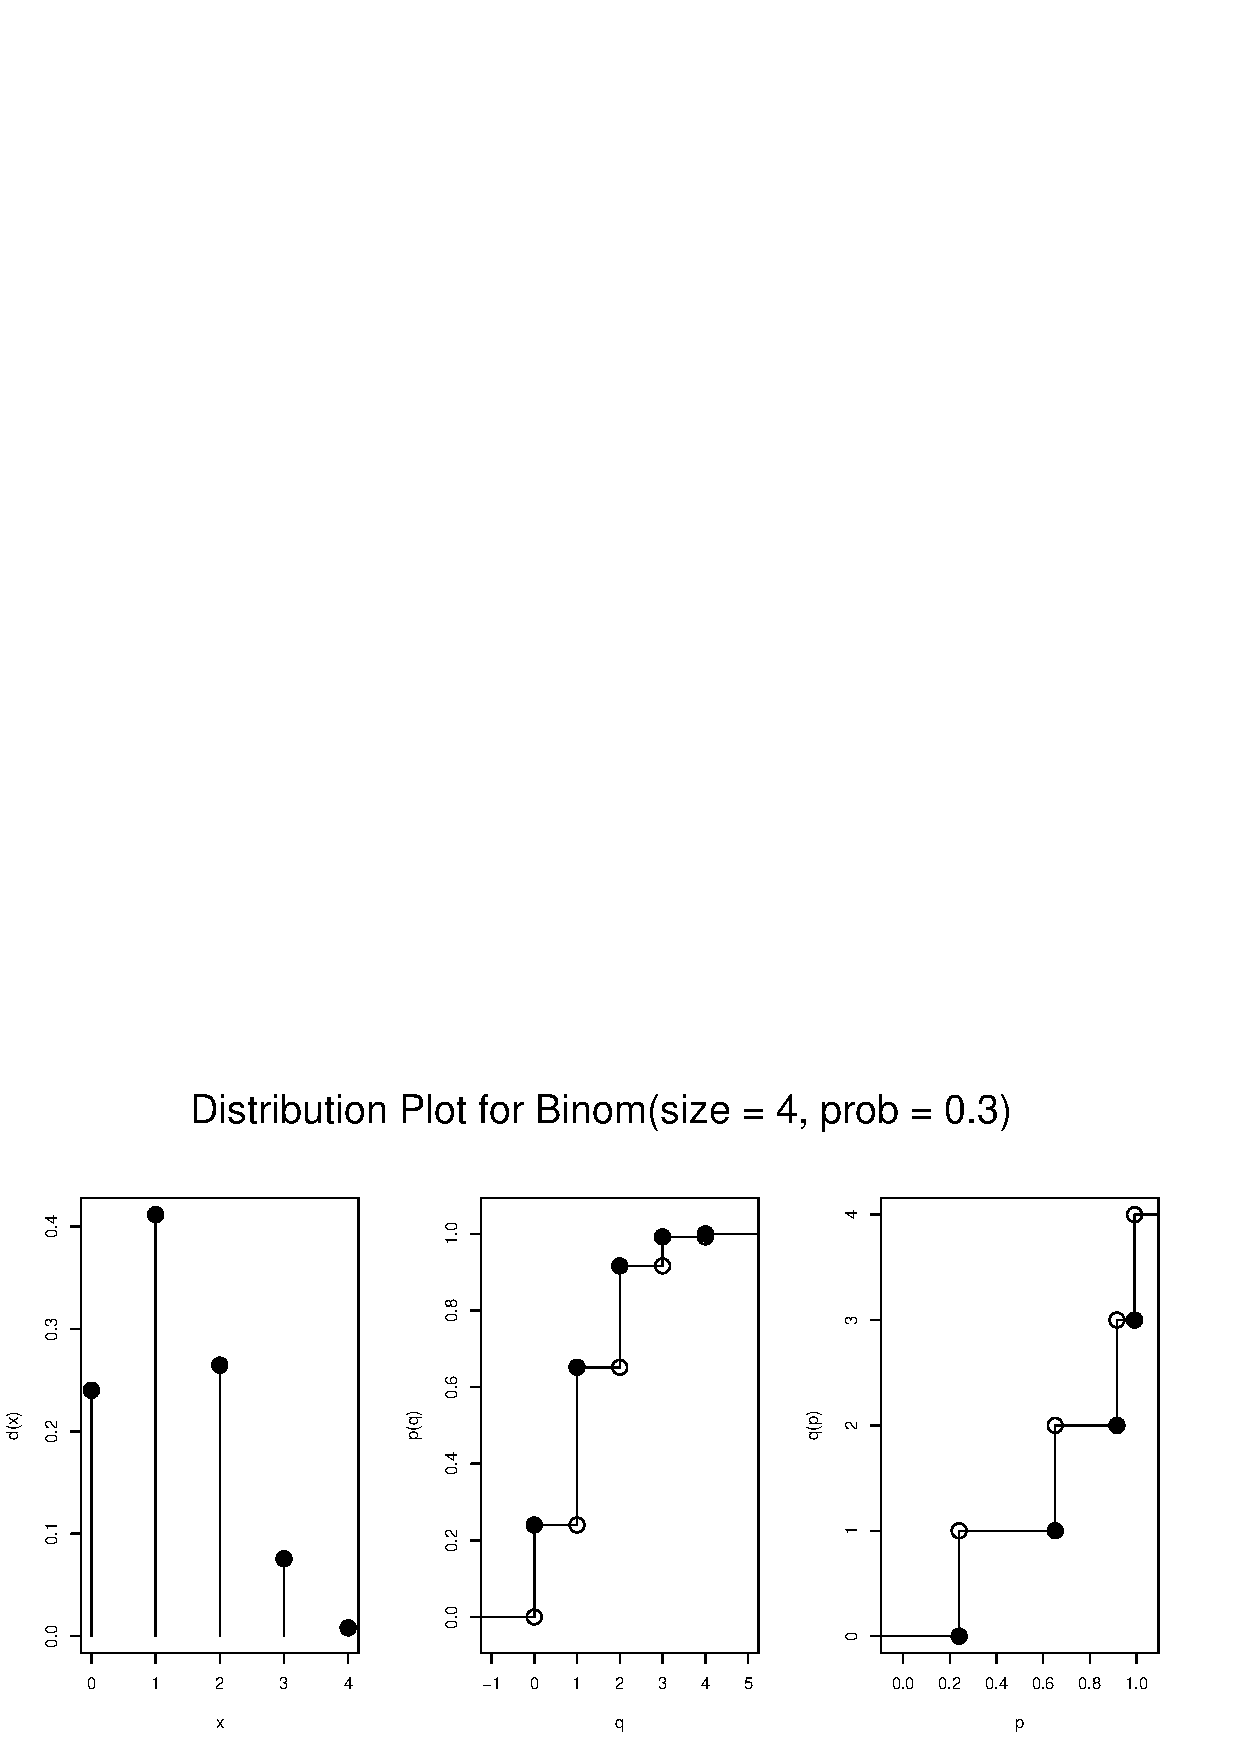
\includegraphics{distr-plotex3}
\end{figure}

\begin{figure}[p]
\begin{Schunk}
\begin{Sinput}
> plot(Binom(size = 4, prob = 0.3), cex.points = 1.2, pch = 20, lwd = 2,
+      withSweave = TRUE)
\end{Sinput}
\end{Schunk}
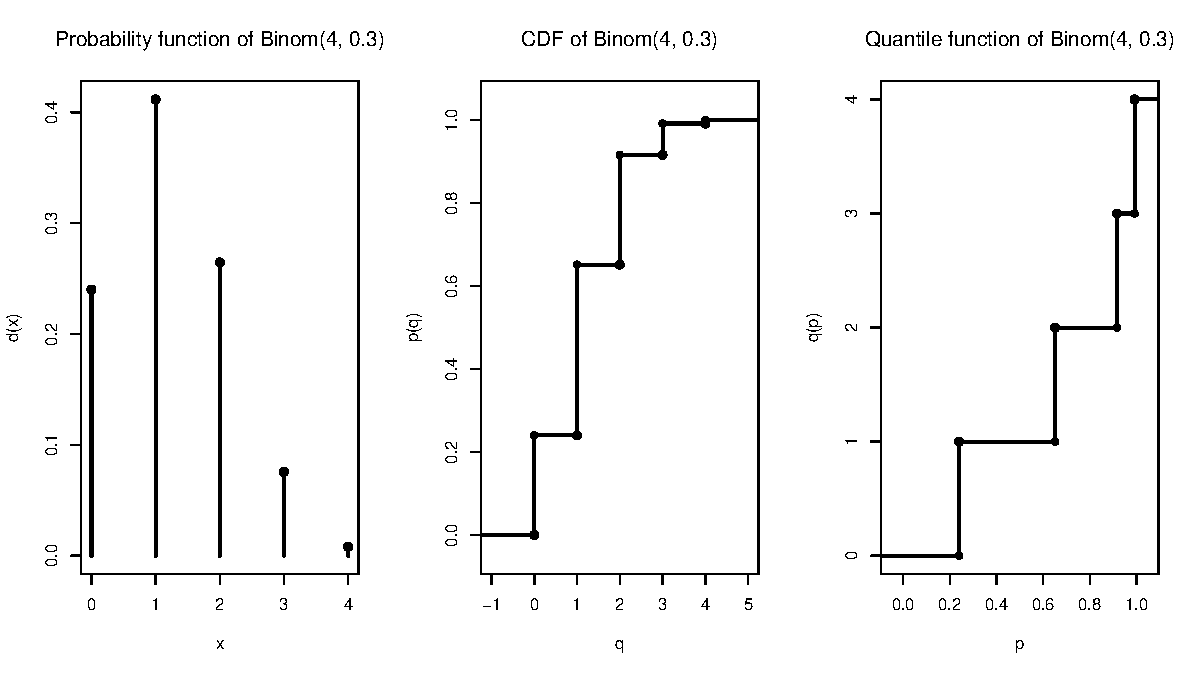
\includegraphics{distr-plotex4}
\end{figure}

\begin{figure}[p]
\begin{Schunk}
\begin{Sinput}
> B <- Binom(size = 4, prob = 0.3)
> plot(B, col="red", col.points = "green", main = TRUE, col.main="blue",
+      col.sub = "orange", sub = TRUE, cex.sub = 0.6, col.inner = "brown",
+      withSweave = TRUE)
\end{Sinput}
\end{Schunk}
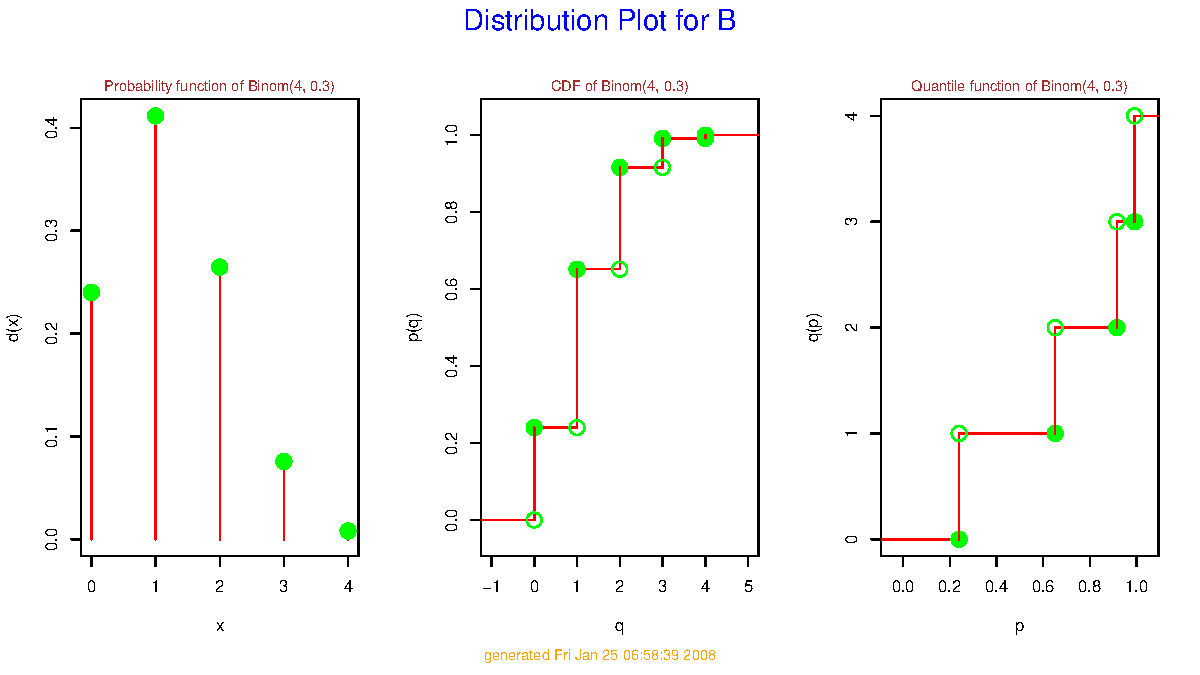
\includegraphics{distr-plotex5}
\end{figure}

\begin{figure}[p]
\begin{Schunk}
\begin{Sinput}
> plot(Nbinom(size = 4,prob = 0.3), cex.points = 1.2, pch.u = 20, pch.a = 10,
+      withSweave = TRUE)
\end{Sinput}
\end{Schunk}

\includegraphics{distr-plotex6}
\end{figure}

\begin{figure}[p]
\begin{Schunk}
\begin{Sinput}
> plot(Chisq(), log = "xy", ngrid = 100, withSweave = TRUE)
\end{Sinput}
\end{Schunk}
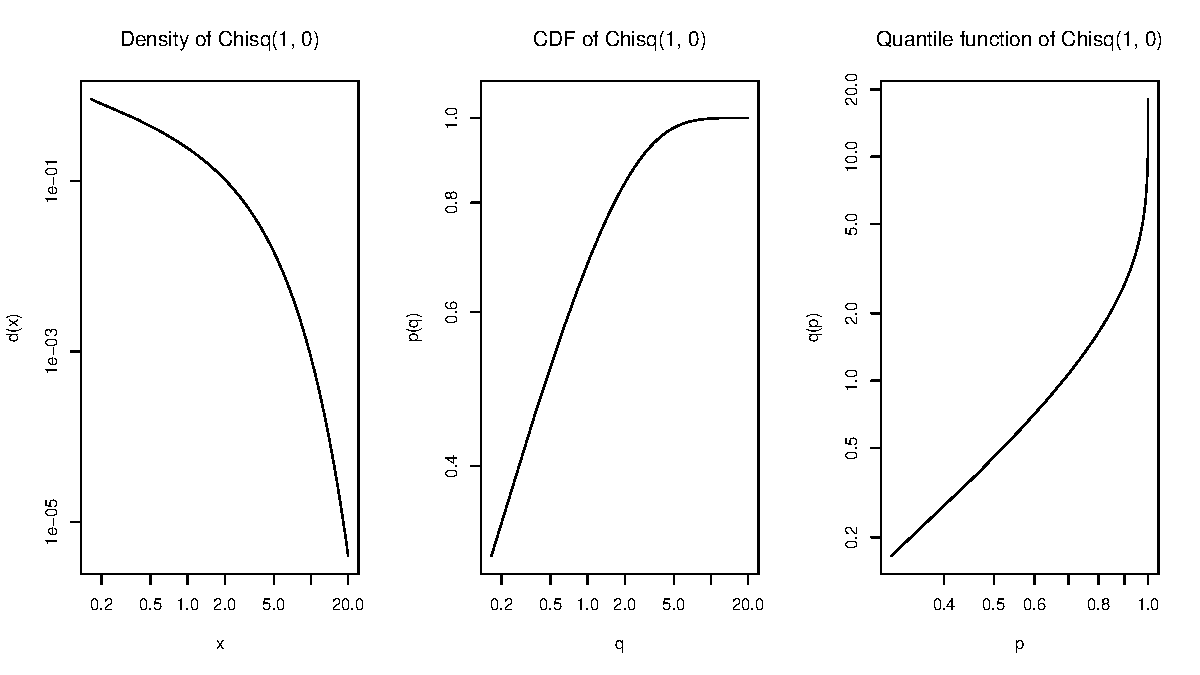
\includegraphics{distr-plotex7}
\end{figure}

\begin{figure}[p]
\begin{Schunk}
\begin{Sinput}
> plot(Norm(), lwd=3, col = "red", ngrid = 200, lty = 3, las = 2,
+      withSweave = TRUE)
\end{Sinput}
\end{Schunk}
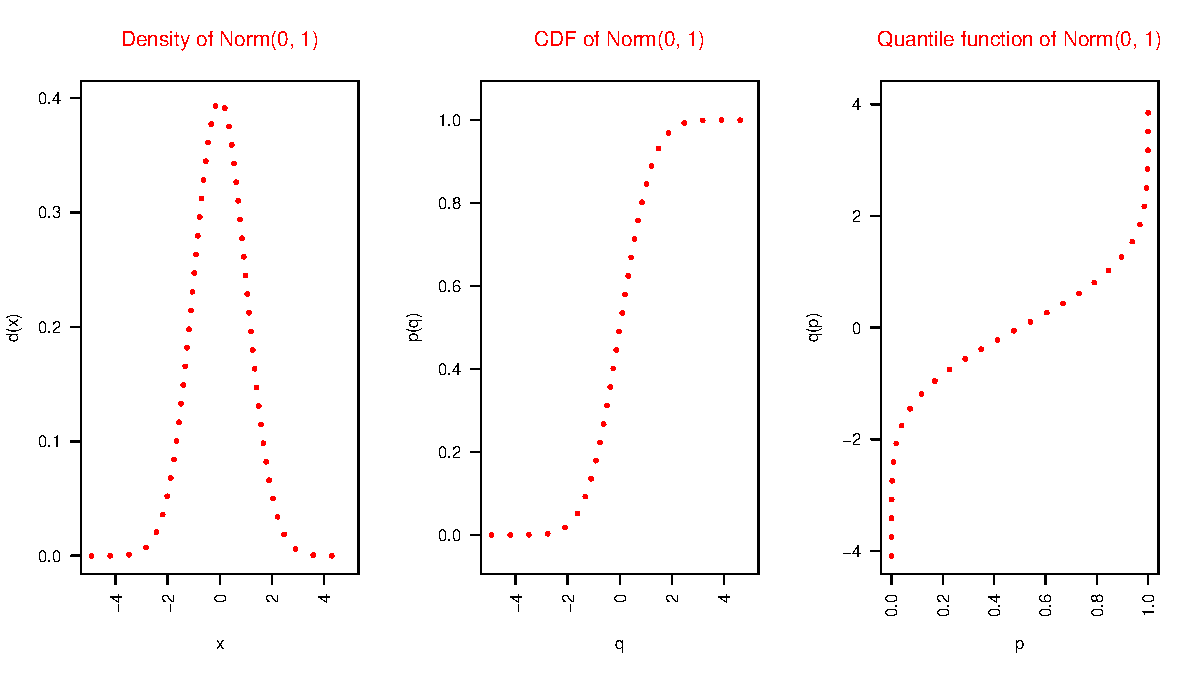
\includegraphics{distr-plotex8}
\end{figure}

\begin{figure}[p]
\begin{Schunk}
\begin{Sinput}
> plot(Norm(), main = "my Distribution: \%A",
+      inner = list(expression(paste(lambda, "-density of \%C(\%P)")), "CDF",
+                   "Pseudo-inverse with param's \%N"),
+      sub = "this plot was correctly generated on \%D",
+      cex.inner = 0.9, cex.sub = 0.8, withSweave = TRUE)
\end{Sinput}
\end{Schunk}
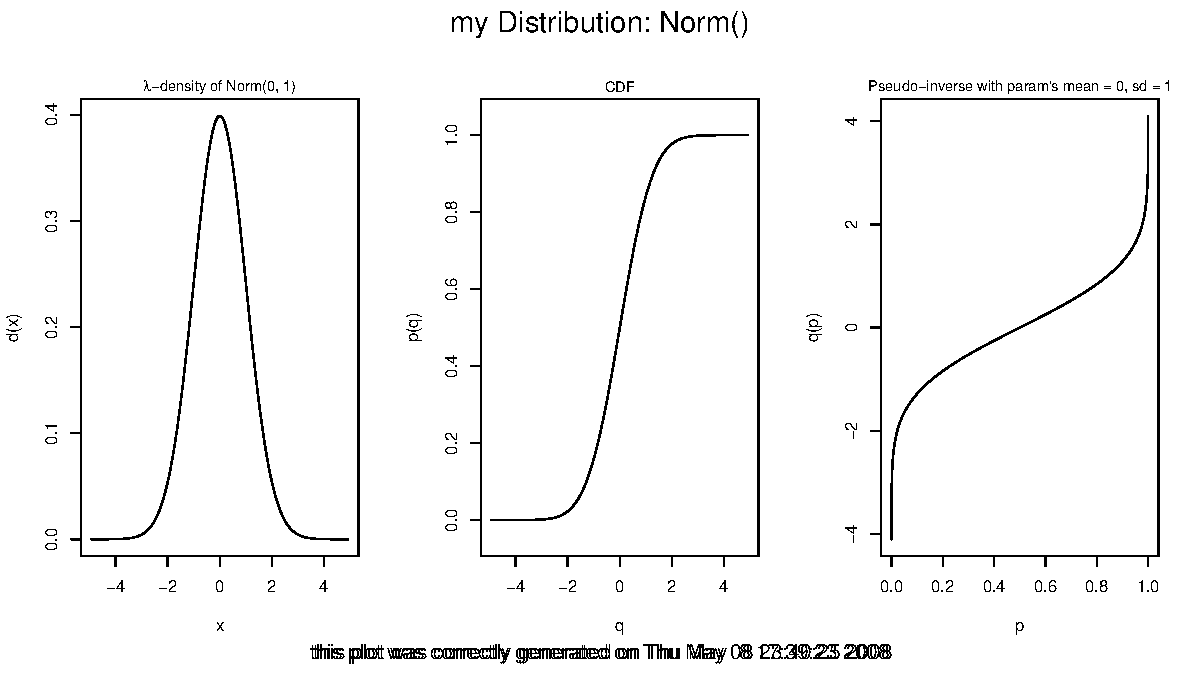
\includegraphics{distr-plotex9}
\end{figure}

\begin{figure}[p]
\begin{Schunk}
\begin{Sinput}
> Ch <- Chisq(); setgaps(Ch, exactq = 3)
> plot(Ch, cex = 1.2, pch.u = 20, pch.a = 10, col.points = "green",
+      col.vert = "red", withSweave = TRUE)
\end{Sinput}
\end{Schunk}
\includegraphics{distr-plotex10}
\end{figure}

\par
For objects of  class \code{Dataclass} ---or of a corresponding subclass---
 \code{plot} plots the sample against the run index and in case  of
 \code{ContSimulation} the contaminating variables are highlighted by a
 different color. Additional arguments controlling
 the plot as in the default \code{plot} command may be passed,
 confer \code{help("plot-methods",package="distrSim")}.
 \par
 For an object of class \code{Evaluation},
\code{plot} yields a boxplot of the results of the evaluation.
For an object of class \code{EvaluationList},
\code{plot} regroups the list according to the different columns/coordinates of
the result of the evaluation; for each such coordinate, a boxplot is generated,
containing possibly several procedures, and, if evaluated at a
\code{Contsimulation}, the plots are also grouped into evaluations on ideal and
real data. As for the usual \code{boxplot} function you may pass additional
``\code{plot}-type'' arguments to this particular \code{plot} method, confer
\code{help("plot-methods",package="distrTEst")}. In particular, the
\code{plot}-arguments \code{main} and \code{ylim}, however, may also be
transmitted coordinatewise, i.e.; a vector of the same length as the dimension
of the result {\tt resDim} (e.g.\ parameter dimension), respectively a
{\tt 2 x resDim} matrix, or they may be transmitted globally, using the
usual {\tt S} recycling rules.
%\newline??????1
\subsection[liesInSupport]{\code{liesInSupport}}
For all discrete distribution classes, we have methods \code{liesInSupport} to
check whether a given vector/ a matrix of points lies in the support of the
distribution.

\subsection[Simulation (in package distrSim)]%
{Simulation (in package \pkg{distrSim})}
%
From version 1.6 on, \code{simulation} is available in package  \pkg{distrSim}.

For the classes \code{Simulation} and \code{ContSimulation}, we normally will
not save the current values of the simulation, as they can easily be reproduced
knowing the values of the other slots of this class.
%
So when declaring a new object of either of the two classes, the slot
\code{Data} will be empty (\code{NULL}).
To fill it with the simulated values, we have to apply the method
\code{simulate} to the object. This has to be redone whenever another slot of
the object is changed.
%
To guarantee reproducibility, we use the slot \code{seed}.\\
%
This slot is controlled and set through
\href{mailto:pgilbert@bank-banque-canada.ca}{Paul Gilbert's} \pkg{setRNG}
package.
By default, \code{seed} is set to \code{setRNG()}, which returns the current
``state'' of the random number generator (RNG). So the user does not need to
specify a value for \code{seed}, and nevertheless may reproduce his samples:
He simply uses \code{simulate} to fill the \code{Data} slot.
If the user wants to, he may also set the \code{seed} explicitly via the
replacement function \code{seed()}, but has to take care of the correct format
himself, confer the documentation of \code{setRNG}. One easy way to fill
the \code{Data} slot of a simulation \code{X} with ``new'' random numbers is
\begin{Schunk}
\begin{Sinput}
> have.distrSim <- suppressWarnings(require("distrSim"))
> if (have.distrSim)
+    {X <- Simulation()
+     seed(X) <- setRNG()
+     simulate(X)
+     print(Data(X)[1:10])
+    } else {
+     cat("\n functionality not (yet) available; ")
+     cat("you have to install package \"distrSim\" first.\n")
+     }
\end{Sinput}
\begin{Soutput}
 [1] -0.662383253  1.348752507 -0.506704107  1.258512234 -0.394878529
 [6] -0.509002453 -0.007476359 -0.590439080  2.212147319  0.694967040
\end{Soutput}
\end{Schunk}
%
\subsection[Evaluate (in package distrTEst)]%
{Evaluate (in package \pkg{distrTEst})}\label{evaluate}
%
From version 1.6 on \code{evaluate} is available in  \pkg{distrTEst}.

In an object of class \code{Evaluation}  we store relevant information
about an evaluation of a statistical procedure (estimator/test/predictor)
on an object of class \code{Dataclass}, including the concrete results of
this evaluation. An object of class \code{Evaluation}  is generated by an
application of method \code{evaluate} which takes as arguments an object of
class  \code{Dataclass} and a procedure of type \code{function}. As an example,
confer Example~\ref{simex}.
For data of class \code{Contsimulation}, the result takes a slightly different,
combining evalations on ideal and real data.
%
\subsection{Is-Relations}
%
By means of \code{setIs}, we have ``told'' {\sf R}  that a distribution object
\code{obj} of class
\begin{itemize}
  \item  \code{"Unif"} with  $\code{Min} \doteq 0$ and  $\code{Max} \doteq 1$
   also is a Beta distribution with parameters \code{shape1 = 1, shape2 = 1}
  \item  \code{"Geom"} also is a negative Binomial distribution with parameters
         \code{size = 1, prob = prob(obj)}
  \item \code{"Cauchy"} with $\code{location} \doteq 0$ and
         $\code{scale}\doteq 1$ also is a T distribution with parameters
         \code{df = 1, ncp = 0}
  \item \code{"Exp"} also is a Gamma distribution with parameters
         \code{shape = 1, scale = 1/rate(obj)} and
         a Weibull  distribution with parameters
         \code{shape = 1, scale = 1/rate(obj)}
  \item \code{"Chisq"} with non-centrality $\code{ncp}\doteq 0$ also is a
        Gamma distribution with parameters \code{shape = df(obj)/2, scale = 2}
  \item \code{"DiscreteDistribution"}  (from version 1.9 on) with an equally
         spaced support also is a \code{"LatticeDistribution"}
\end{itemize}
%
\subsection{Further methods}
%
When iterating/chaining mathematical operations on a univariate distribution,
generation process of random variables can become clumsy and slow.
To cope with this, we introduce a sort of ``Forget-my-past''-method
\code{simplifyr} that replaces the  chain of mathematical operations in
the \code{r}-method by drawing with replacement from a large
sample ($10^{\tt RtoDPQ.e}$) of these.
%
\subsection[Functionals (in package distrEx)]%
{Functionals (in package \pkg{distrEx})}\label{Functionals}
%
\subsubsection{Expectation}
The most important contribution of package \pkg{distrEx} is a general
expectation operator. In basic statistic courses, the expectation
${\rm E}$ may come as ${\rm E}\,[X]$, ${\rm E}\,[f(X)]$, ${\rm E}\,[X|Y=y]$,
or ${\rm E}\,[f(X)|Y=y]$. Our operator (or in S4-language ``generic function'')
\code{E} covers all of these situtations (or {\it signatures\/}).
\paragraph{default call}
The most frequent call will be \code{E(X)} where \code{X} is an (almost)
arbitrary distribution object.
More precisely, if \code{X} is of a specific distribution class like
\code{Pois}, it is evaluated exactly using analytic terms. Else if it is of
class \code{DiscreteDistribution} we use a sum over the support of \code{X},
and if it is of class \code{AbscontDistribution} we use numerical
integration\footnote{i.e., we first try (really(!): \code{try})
\code{integrate} and if this fails we use Gau{\ss}-Legendre integration
according to \cite{NumR:92}, see also \code{?distrExIntegrate}};
for {\tt X} of class \code{UnivarLebDecDistribution}, expectations
for discrete and absolutely continuous part are evaluated separately and
subsequently combined according to their respective weights.
If we only  know that {\tt X} is of class \code{UnivariateDistribution} we
use Monte-Carlo
integration. This also is the default method in for class
\code{MultivariateDistribution}, while for \code{DiscreteMVDistribution} we
again use sums. For an object \code{Y} of a subclass of class
union \code{AffLinDistribution}, we determine the expectation as
\code{Y@a * E(Y@X0) + Y@b} and hence use analytic terms for \code{X0} if
available.

\paragraph{with a function as argument}
 we proceed just as without: if \code{X} is of class\linebreak[4]
 \code{DiscreteDistribution}, we use a sum over the support of \code{X},
and if \code{X} is of class\linebreak[4] \code{AbscontDistribution} we use numerical
integration; else we use Monte-Carlo integration.
\paragraph{in addition: with a condition as argument} we simply use the
corresponding \code{d} respective \code{r} slots with the additional
argument \code{cond}.
\paragraph{exact evaluation}
is available for \code{X} of class \code{Beta} (for noncentrality $0$),
\code{Binom}, \code{Cauchy}, \code{Chisq}, \code{Dirac}, \code{Exp}, \code{Fd},
\code{Gammad}, \code{Geom}, \code{Hyper}, \code{Logis}, \code{Lnorm},
\code{Nbinom}, \code{Norm}, \code{Pois}, \code{Td}, \code{Unif}, \code{Weibull}.
\paragraph{examples} $ \mbox{ }$\newline
\begin{Schunk}
\begin{Sinput}
> have.distrEx <- suppressWarnings(require("distrEx"))
> if (have.distrEx)
+     {D4 <- LMCondDistribution(theta = 1)
+      D4  # corresponds to Norm(cond, 1)
+      N <- Norm(mean = 2)
+
+      print(E(D4, cond = 1))
+      print(E(D4, cond = 1, useApply = FALSE))
+      print(E(as(D4, "UnivariateCondDistribution"), cond = 1))
+      print(E(D4, function(x){x^2}, cond = 2))
+      print(E(D4, function(x){x^2}, cond = 2, useApply = FALSE))
+      print(E(N, function(x){x^2}))
+      print(E(as(N, "UnivariateDistribution"), function(x){x^2},
+        useApply = FALSE)) # crude Monte-Carlo
+      print(E(D4, function(x, cond){cond*x^2}, cond = 2,
+        withCond = TRUE))
+      print(E(D4, function(x, cond){cond*x^2}, cond = 2,
+        withCond = TRUE, useApply = FALSE))
+      print(E(N, function(x){2*x^2}))
+      print(E(as(N, "UnivariateDistribution"), function(x){2*x^2},
+        useApply = FALSE)) # crude Monte-Carlo
+      Y <- 5 * Binom(4, .25) - 3
+      print(Y); print(E(Y))
+     } else {
+     cat("\n functionality not (yet) available; ")
+     cat("you have to install package \"distrEx\" first.\n")
+     }
\end{Sinput}
\begin{Soutput}
[1] 0.9999998
[1] 0.9999998
[1] 0.9984173
[1] 4.999993
[1] 4.999993
[1] 4.999993
[1] 4.97194
[1] 9.999987
[1] 9.999987
[1] 9.999987
[1] 9.985442
Distribution Object of Class: AffLinLatticeDistribution
[1] 2
\end{Soutput}
\end{Schunk}
%
%
\subsubsection{Variance}
The next-common functional is the variance. In order to keep a unified
notation we will use the same name as for the empirical variance, i.e.,
 \code{var}.
\paragraph{masking \pkg{stats}-method \code{var}}
To cope with the different argument structure of the empirical variance,
i.e. \code{var(x, y = NULL, na.rm = FALSE, use)}  and our functional variance,
i.e.,
\code{var(x, fun = function(t) {t}, cond, withCond = FALSE, useApply = TRUE, ...)}
we have to mask the original \pkg{stats}-method:
\begin{Schunk}
\begin{Sinput}
>   var <- function(x , ...)
+        {dots <- list(...)
+         if(hasArg(y)) y <- dots$"y"
+         na.rm <- ifelse(hasArg(na.rm), dots$"na.rm", FALSE)
+         if(!hasArg(use))
+              use <- ifelse (na.rm, "complete.obs","all.obs")
+         else use <- dots$"use"
+         if(hasArg(y))
+            stats::var(x = x, y = y, na.rm = na.rm, use)
+         else
+            stats::var(x = x, y = NULL, na.rm = na.rm, use)
+         }
\end{Sinput}
\end{Schunk}
before registering \code{var} as generic function.
Doing so, if the \code{x} (or the first) argument of \code{var}
is not of class \code{UnivariateDistribution}, \code{var} behaves identically to
the \pkg{stats} package
\paragraph{default method} if \code{x} is of class \code{UnivariateDistribution},
\code{var} just returns the variance of distribution \code{X} --- or
of \code{fun(X)} if a function is passed as argument fun, or, if a condition
argument \code{cond} (for $Y=y$),  ${\rm Var}\,[X|Y=y]$ respectively
${\rm Var}\,[f(X)|Y=y]$ --- just as for \code{E}. \\
For an object \code{Y} of a subclass of class
union \code{AffLinDistribution}, we determine the variance as
\code{Y@a\textasciicircum2 * var(Y@X0)} and hence use analytic terms for \code{X0} if
available.
\paragraph{exact evaluation} is provided for specific distributions if no
function and no condition argument is given:
this is available for \code{X} of class \code{Beta} (for noncentrality $0$),
\code{Binom}, \code{Cauchy}, \code{Chisq},\code{Dirac}, \code{Exp}, \code{Fd},
\code{Gammad}, \code{Geom}, \code{Hyper}, \code{Logis}, \code{Lnorm},
\code{Nbinom}, \code{Norm}, \code{Pois}, \code{Unif}, \code{Td}, \code{Weibull}.
\subsubsection{Further functionals}
By the same techniques we provide the following functionals for univariate
distributions:
\begin{itemize}
  \item standard deviation: \code{sd}
  \item skewness: \code{skewness}
  (code contributed by G. Jay Kerns, {\small \tt gkerns@ysu.edu})
  \item kurtosis: \code{kurtosis}
   (code contributed by G. Jay Kerns, {\small \tt gkerns@ysu.edu})
  \item median: \code{median} (not for function/condition arguments)
  \item median of absolute deviations: \code{mad} (not for function/condition
  arguments)
  \item interquartile range: \code{IQR} (not for function/condition arguments)
\end{itemize}
%
\subsection[Truncated moments (in package distrEx)]{Truncated moments
(in package \pkg{distrEx})}\label{m1df}
%
For Robust Statistics, the first two truncated moments are very useful. These
are realized as generic functions \code{m1df} and \code{m2df}: They use the
expectation operator for general univariate distributions, but are overloaded
for most specific distributions:
\begin{itemize}
  \item \code{Binom}
  \item \code{Pois}
  \item \code{Norm}
  \item \code{Exp}
  \item \code{Chisq}
\end{itemize}
%
\subsection[Distances (in package distrEx)]{Distances (in package %
 \pkg{distrEx})}\label{Distances}
%
For several purposes like Goodness-of-fit tests or minimum-distance estimators,
distances between distributions are useful. This applies in particular to Robust
Statistics. In package \pkg{distrEx}, we provide the follwoing distances:
\begin{itemize}
  \item Kolmogoroff distance
  \item total variation distance
  \item Hellinger distance
  \item Cram\'er von Mises distance
  \item convex-contamination ``distance'' (asymmetric!) defined as
  $$
d(Q,P):=\inf\{r>0\,|\, \exists \;\mbox{probability } H:\quad Q=(1-r)P+rH \}
  $$
\end{itemize}
\subsection[Functions for demos (in package distrEx)]{Functions for demos
(in package \pkg{distrEx})}\label{Demos}
%
To illustrate the possibilities with packages \pkg{distr} and \pkg{distrEx} we
include two major demos to \pkg{distrEx}, each with extra code to it ---
one for the CLT and one for the LLN.

From version 2.0 on, we have started a new package \pkg{distrTeach}, which
is to use the capabilities of packages \pkg{distr} and \pkg{distrEx} for
illustrating topics of Stochastics and Statistics as taught in secondary
school. So far we have moved the illustrations for the CLT and the LLN
just mentioned to it.

\subsubsection{CLT for arbitrary summand distribution}

By means of our convolution algortithm as well as with the operators \code{E}
and \code{sd} an illustration for the CLT is readily written:
function \code{illustrateCLT}, respectively demo \code{illustCLT}.
For plotting, we have particular methods for discrete and absolute continuous
distributions. The user may specify a given summand distribution, an upper
limit for the consecutive sums to be considered and a pause between the
corresponding plots in seconds. From version 1.9 on, we also include a
\code{TclTk}-based version of this demo, where the user may enter the
distribution argument (i.e.; the summands' distribution) into a text line and
control the sample size by a slider in some widget: \code{illustCLT\_tcl}
From version 2.0 on, this functionality has moved to package \pkg{distrTeach}.

\subsubsection{LLN for arbitrary summand distribution}

From version 1.9 on, similarly, we provide an illustration for the LLN:
function \code{illustrateLLN}, respectively demo \code{illustLLN}.
The user may specify a vector of sample sizes to be
considered, the number of replicates to be drawn and a pause between the
corresponding plots in seconds, also, optionally, the limiting expectation
(in case of class \code{Cauchy}: the non-limiting median) is drawn as a line and
Chebyshev/CLT-based (pointwise) confidence bands and their respective empirical
coverages are displayed.
From version 2.0 on, this functionality has moved to package \pkg{distrTeach}.

\subsubsection{Deconvolution example}

To illustrate conditional distributions and their implementation in
\linebreak[4]\pkg{distrEx}, we consider the following situation:
We consider a signal $X\sim P^X$ which is disturbed by noise
$\varepsilon\sim P^\varepsilon$, independent from $X$; in fact we observe
$Y=X+\varepsilon$ and want to reconstruct $X$ by means of $Y$. By means of the
generating function \code{PrognCondDistribution}
of package \pkg{distrEx}, for absolutely continuous $P^X, P^\varepsilon$, we may
determine the factorized conditional distribution $P^{X|Y=y}$, and based on this
either its (posterior) mode oder (posterior) expectation; also see
\code{demo(Prognose, package="distrEx")}.

%
\section[New package distrMod]{New package {\tt distrMod}}\label{distrMod}
%
\subsection{Model Classes}
%
[[[[MATTHIAS]]]
\subsection{Estimator Classes}
%
[[[[MATTHIAS]]]
%
\subsection{Minimum Criterium Estimation}
%
[[[[MATTHIAS]]]
%
%
\section{Options}\label{options}
%
%
\subsection[Options for distr]{Options for \pkg{distr}}
%
Analogously to the \code{options} command in {\sf R} you may specify a number of
global ``constants'' to be used within the package. These include
\begin{itemize}
  \item \code{DefaultNrFFTGridPointsExponent}: the binary logarithm of the
        number of grid-points used in FFT ---default $12$
  \item \code{DefaultNrGridPoints}: number of grid-points used for a continuous
        variable ---default $4096$
  \item \code{DistrResolution}: the finest step length that is permitted for a
        grid for a discrete variable ---default $1{\rm e-}\!06$
  \item \code{RtoDPQ.e}: For simulational determination of \code{d}, \code{p}
         and \code{q}, $10^{\rm RtoDPQ.e}$ random variables are
  simulated ---default $5$
  \item \code{TruncQuantile}: to work with compact support, random variables are
        truncated to their lower/upper
  \code{TruncQuantile}-quantile   ---default $1{\rm e-}\!05$.\\
  From version 1.9 on, for $\varepsilon={\tt \code{TruncQuantile}}$, we use calls of form
  \code{q(X)(eps, lower.tail = FALSE)} instead of   \code{q(X)(1-eps)} to gain higher
  precision.
  \item \code{warningSim}: controls whether a warning issued at printing/showing
        a \code{Distribution} object the slots of which have been
  filled starting with simulations ---default \code{TRUE}
  \item \code{warningArith}: controls whether a warning issued at
   printing/showing a \code{Distribution} object produced by arithmetics
  operating on distributions ---default \code{TRUE}
  \item \code{withgaps}: controls whether in the return value of arithmetic
  operations the slot \code{gaps} of an the \code{AbscontDistribution} part
  is filled automatically based on empirical evaluations via  \code{setgaps}
   ---default \code{TRUE}
  \item \code{simplifyD}: controls whether in the return value of arithmetic
  operations there is a call to \code{simplifyD} or not ---default \code{TRUE}
\end{itemize}
All current options may be inspected by \code{distroptions()}  and modified by
 \linebreak[4] \code{distroptions("<options-name>"=<value>)}.\\
As \code{options},  \code{distroptions("<options-name>")} returns a list of
 length $1$ with the value of the corresponding option,
so here, just as \code{getOption},  \code{getdistrOption("<options-name>")} will
 be preferable, which only returns the value.
%\newline0??????
\subsection[Options for distrEx]{Options for \pkg{distrEx}}\label{distrExoptions}
Up to version {\tt 0.4-4} we used the function
 \code{distrExOptions(arg = "missing", value = -1)} to manage some global
 options for \pkg{distrEx}, i.e.:\\
\code{distrExOptions()} returns a list of these options,
\code{distrExOptions(arg=x)} returns option \code{x}, and
\code{distrExOptions(arg=x,value=y)} sets the value of option \code{x} to
 {\tt y}.\\
 From version {\tt 1.9} on, we use a mechanism analogue to the
  \code{distroptions}/\code{getdistrOption} commands:
You may specify certain
global output options to be used within the package with
 \code{distrExoptions}/\code{getdistrExOption}. These include
\begin{itemize}
  \item \code{MCIterations}: number of Monte-Carlo iterations used for crude
          Monte-Carlo integration.
  \item \code{GLIntegrateTruncQuantile}: If \code{integrate} fails and there are
          infinite integration limits, the function \code{GLIntegrate} is
          called inside of \code{distrExIntegrate} with the corresponding
          quantiles  \code{GLIntegrateTruncQuantile} resp.\
          \code{1-GLIntegrateTruncQuantile} as finite integration limits.
  \item \code{GLIntegrateOrder}: The order used for the Gau{\ss{}}-Legendre
          integration inside of \code{distrExIntegrate}.
  \item \code{ElowerTruncQuantile}: The lower limit of integration used inside
       of \code{E} which corresponds to the \code{ElowerTruncQuantile}-quantile.
  \item \code{EupperTruncQuantile}: The upper limit of integration used inside
          of \code{E} which corresponds to the
          \code{(1-ElowerTruncQuantile)}-quantile.
  \item \code{ErelativeTolerance}: The relative tolerance used inside of
        \code{E} when calling\linebreak[4] \code{distrExIntegrate}.
  \item \code{m1dfLowerTruncQuantile}: The lower limit of integration used
        inside of \code{m1df} which corresponds to the
          \code{m1dfLowerTruncQuantile}-quantile.
  \item \code{m1dfRelativeTolerance}: The relative tolerance used inside of
          \code{m1df} when calling \code{distrExIntegrate}.
  \item \code{m2dfLowerTruncQuantile}: The lower limit of integration used
        inside of \code{m2df} which corresponds to the
          \code{m2dfLowerTruncQuantile}-quantile.
  \item \code{m2dfRelativeTolerance}: The relative tolerance used inside of
          \code{m2df} when calling \code{distrExIntegrate}.
\end{itemize}

%We are planning to switch to \code{distroptions}/\code{getdistrOption}-like
% commands in the next release of this package.
%
\subsection[Options for distrSim]{Options for \pkg{distrSim}}
Just as with to the \code{distroptions}/\code{getdistrOption} commands you
may specify certain global output options to be used within the package with
\code{distrSimoptions}/\linebreak[4] \code{getdistrSimOption}. These include
\begin{itemize}
  \item \code{MaxNumberofPlottedObs} the maximal number of observation plotted
  in a plot of an object of class \code{Dataclass}; defaults to 4000

  \item \code{MaxNumberofPlottedObsDims}: the maximum number of observations to
  be plotted in a plot of an object of class \code{Dataclass}
  and descendants; defaults to 6.
  \item \code{MaxNumberofPlottedRuns}: the maximum number of runs to be plotted
  in a plot of an object of class \code{Dataclass}
  and descendants (one run/panel); defaults to 6.
  \item \code{MaxNumberofSummarizedObsDims}: the maximum number of observations
  to be summarized of an object of class \code{Dataclass}
  and descendants; defaults to 6.
  \item \code{MaxNumberofSummarizedRuns}: the maximum number of runs to be
   summarized of an object of class \code{Dataclass}
  and descendants; defaults to 6.
\end{itemize}
%
\subsection[Options for distrTEst]{Options for \pkg{distrTEst}}
Just as with to the \code{distroptions}/\code{getdistrOption} commands you may
specify certain
global output options to be used within the package with
\code{distrTEstoptions}/ \linebreak[4]\code{getdistrTEstOption}. These include
\begin{itemize}
  \item \code{MaxNumberofPlottedEvaluations}:  the maximal number of evaluations
  to be plotted
  in a plot of an object of class \code{EvaluationList}; defaults to 6
  \item \code{MaxNumberofPlottedEvaluationDims}: the maximal number of
   evaluation dimensions to be plotted in a plot of an
         object of class \code{Evaluation}; defaults to 6
  \item \code{MaxNumberofSummarizedEvaluations}: the  maximal number of
  evaluations to be summarized of an object of class
  \code{EvaluationList}; defaults to 15
  \item \code{MaxNumberofPrintedEvaluations}: the maximal number of evaluations
   printed of an object of class
  \code{EvaluationList}; defaults to 15
\end{itemize}

%??????1

\section{Startup Messages}
%
For the management of startup messages, from version~1.7, we use package
\pkg{startupmsg}:
When loading/attaching packages \pkg{distr}, \pkg{distrEx}, \pkg{distrSim}, or
\pkg{distrTEst} for each package a disclaimer is displayed.

You may suppress these start-up banners/messages completely by setting
\linebreak[4]\code{options("StartupBanner"="off")}
somewhere before loading this package by \code{library} or \code{require} in
your R-code / R-session.

If option \code{"StartupBanner"} is not defined (default) or setting\linebreak[4]
\code{options("StartupBanner" = NULL)} or %\linebreak[4]
\code{options("StartupBanner" = "complete")}
the complete start-up banner is displayed.

For any other value of option \code{"StartupBanner"} (i.e., not in
\linebreak[3]\code{c(NULL, "off", "complete")})
only the version information is displayed.

The same can be achieved by wrapping the \code{library} or \code{require}
call into either
 \linebreak[4]\code{onlytypeStartupMessages(<code>, atypes="version")}
 or\linebreak[4] \code{suppressStartupMessages(<code>)}.
%

\section[System/version requirements]{System/version requirements, license,
 etc.\ }
%
\subsection{System requirements}
%
As our package is completely written in {\sf R}, there are no dependencies
on the underlying OS; of course, there is the usual speed gain
possible on recent machines. We have tested our package on a Pentium~II with
 233 MHz, on Pentium~III's with 0.8--2.1 GHz, and on an Athlon with 2.5 GHz
 giving a reasonable performance.

\subsection{Required version of {\sf R}}
Contrary to the hardware required,
if you want to use \code{library} or \code{require} to use  \pkg{distr}
within {\sf R} code, you need at least {\sf R} Version {\tt 1.8.1},
as we make use of name space operations only available from that version on;
also, the command \code{setClassUnion}, which is used in some sources, is only
 available from that version on.\\
%
On the other hand, if the package may be pasted in by \code{source}, the code
works with {\sf R} from
version {\tt 1.7.0} on ---but without using name-spaces, which is only available
 from {\tt 1.8.0} on.
Due to some changes in {\sf R} from version {\tt 1.8.1} to {\tt 1.9.0} and from
{\tt 1.9.1} to {\tt 2.0.0}, we have to provide different
 {\tt zip}/{\tt tar.gz}-Files for these versions.\\
Versions of \pkg{distr} from version number {\tt 1.5} onwards are only
supplied for {\sf R} Version {\tt 2.0.1 patched} and later.
After a reorganization, versions of \pkg{distr} from version number {\tt 1.6}
onwards are only supplied for {\sf R} Version {\tt 2.2.0 patched} and later.


\subsection{Dependencies}
In package \pkg{distr}, from version 2.0, we make use of \code{D1ss} from
\href{mailto:maechler@stat.math.ethz.ch}{Martin M\"achler's} package \pkg{sfsmisc}.
In package \pkg{distrEx}, we need
\href{mailto:alec_stephenson@hotmail.com}{Alec Stephenson's} package \pkg{evd}
for the extreme  value distributions implemented therein.
In package \pkg{distrSim}, and conseqently also in package \pkg{distrTEst} we
use \href{mailto:pgilbert@bank-banque-canada.ca}{Paul Gilbert's}
package \pkg{setRNG}
to be installed from \href{http://cran.r-project.org/mirrors.html}{\tt CRAN}
for the control of the seed of the random number generator in our simulation
classes.
More precisely, for our version $\le$ {\tt 1.6}  we need his
 version $<$ {\tt 2006.2-1},
and for our version $\ge$ {\tt 1.7} we need his version $\ge$ {\tt 2006.2-1}.

From package version {\tt 1.7}/{\tt 0.4-3} on, we also need package
 \pkg{startupmsg} by the first of the present authors, which also is available
 on \href{http://cran.r-project.org/mirrors.html}{\tt CRAN}.

\subsection{License}
This software is distributed under the terms of the GNU GENERAL
PUBLIC LICENSE Version 2, June 1991, confer\newline
%\href{http://www.gnu.org/copyleft/gpl.html}%
%{\tt http://www.gnu.org/copyleft/gpl.html}
\href{http://www.gnu.org/copyleft/gpl.html}%
{\footnotesize \tt http://www.gnu.org/copyleft/gpl.html}

\section{Details to the implementation}
\begin{itemize}
\item As the normal distribution is closed under affine transformations, we have
overloaded the corresponding methods.
%The same goes for the exponential distribution under scale transformations.
\item For the general convolution algorithm for univariate probability
distribution functions/densities by means of FFT, which we use in the
overloaded {\tt "+"}-operator, confer~\cite{K:R:S:04}.
\item Exact convolution methods are implemented for the normal, the Poisson,
the binomial, the negative binomial, the Gamma (and the \code{Exp}), and
the {$\chi^2$} distribution
\item Exact formulae for scale transformations are implemented for
the Exp-/Gamma-distribution, the Weibull and the log-normal distribution
(the latter two from version 1.9 on).
\item Exact formulae for affine linear transformations are available for
the normal, the logistic and the Cauchy distribution (the latter two from
version 1.9 on).
\item Instances of any class transparent to the user are initialized
by\linebreak[4] {\tt<classname>([<slotname>=<value>,...])}
where except for class \code{DataClass} in package \pkg{distrSim} all classes
have default values for all their slots; in \code{DataClass},
the slot \code{Data} has to be specified.
\item Multiplication (and Division) is implemented as corresponding
exponentials of the convolution of the logarithms (evaluated separately
for positive and negative parts).
\item Exponentiation also uses the exp-log trick.
\item Multiplication, Exponentation, and Min/Maximum of an \code{AbscontDistribution}
and a \code{DiscreteDistribution} as an intermediate step produce
a \code{UnivarMixingDistribution}, with one mixing component for each element
of the support of the \code{DiscreteDistribution}. As a last step,
this \code{UnivarMixingDistribution} is then ``flattened''.
\item
As suggested in \cite{OOPGent} all slots are accessed and modified by
corresponding accessor- and replacement functions ---templates for which were
produced by \code{standardMethods}.

{\bf We strongly discourage the use of the \code{@}-operator to modify
or even access slots \code{r}, \code{d}, \code{p}, and \code{q}, confer
Example~{\ref{destrex}}.}
\end{itemize}
%
\section{A general utility}
%
Following \cite{OOPGent}, the programmer of {\tt S4}-classes should provide
accessor and replacement functions for the inspection/modification of
any newly introduced slot. This can be quite a task when you have a
lot of classes/slots.
As these functions all have the same structure, it would be nice
to automatically generate templates for them.
Faced with this problem in developing this package, Thomas Stabla
has written such a utility, \code{standardMethods} ---which the authors
of this package recommend for any developer of {\tt S4}-classes.
For more details, see \code{?standardMethods}.

\section{Odds and Ends}
\subsection[What should be done and what we could do]%
{What should be done and what we could do ---for version $>$\pkgversion}
\begin{itemize}
\item application of analytic FourierTransforms instead of FFT where
appropriate ---perhaps also to be controlled
by a parameter/option
\item use the \code{q}-slot applied to \code{runif} in \code{simplifyr}
for continuous distributions
\item further exact formulae for binary arithmetic operations like \code{"*"}
%\item derivation of a class \code{LatticeDistribution} from
%\code{DiscreteDistribution} to be able to easily apply FFT
%\item redo the math-method for discrete distributions when only slot \code{r} %
%is given
%\item better documentation for method \code{evaluate} / class \code{Evaluation}
%\item adaptation of class \code{Evaluation} / method \code{evaluate} to be more flexible
%\item use of  \code{initialize} in generating functions
%\item generating function for new distribution classes to ease inclusion of
%new distributions
\item goodness of fit tests for distribution-objects
%\item use of $\tt \backslash$\code{S4method} in documentation
%\item overloading binary operators of group \code{Math2} for independent
%distributions
\item defining a subgroup of \code{Math2} of invertible binary operators
%%\item better use of \code{concept} in rd-files
%\item suggestion by \href{mailto:kouros.owzar@duke.edu}{Kouros Owzar}:
%in case of parameters of dimension $p>1$
%---as in case of ${\cal N}(\mu,\sigma^2)$--- possibility to %
%access/replace that parameter  as a vector
\end{itemize}
\subsection{What should be done but for which we lack the know-how}
\begin{itemize}
  \item multivariate distributions
  \item conditional distributions
  \item copula
\end{itemize}
%
\section{Acknowledgement}
In order to give our acknowledgements their due place
in the manual, we insert them before some rather
extensive presentation of examples, because otherwise
they would probably get lost or overseen by most of the
readers.

We thank Martin M\"achler and Josef Leydold for their
helpful suggestions in conceiving the package.
John Chambers also gave several helpful hints and
insights when responding to our requests concerning the
{\tt S4}-class concept in {\tt r-devel}/ {\tt r-help}.
We got stimulating replies to an RFC on {\tt r-devel} by
Duncan Murdoch and Gregory Warnes.
We also thank Paul Gilbert for drawing our attention to his package
 {\tt setRNG} and making it available as stand-alone version.
In the last few days before the release on {\tt CRAN}, Kurt Hornik and
Uwe Ligges were very kind, helping us to find the clue how to
pass all necessary checks by {\tt R CMD check}.
We also thank G. Jay Kerns for contributing code for
the skewness and kurtosis functionals.

Last not least a big "thank you" to Torsten Hothorn as editor
of {\tt R-News}, for his patience with our endless versions
until we finally came to a publishable version.
%\input{distrack}
%
\section{Examples}
\subsection{$12$-fold convolution of uniform $(0,1)$ variables}
\begin{footnotesize}
  Code also available under\newline %
  {\href{http://www.uni-bayreuth.de/departments/math/org/mathe7/DISTR/NormApprox.R}%
  {\parbox[t]{12cm}{$\mbox{\hspace{2cm}}$%
  {\tt http://www.uni-bayreuth.de/departments/math/org/}\\%
  {$\mbox{\hspace{2cm}}$\hphantom{\tt http:/}%
  {\tt /mathe7/DISTR/NormApprox.R}}}}}\\[2ex]
\end{footnotesize}
\begin{small}
  This example shows how easily we may get the distribution of the sum of $12$
  ${\rm i.i.d.}$ ${\rm ufo}(0,1)$--variables minus $6$--- which was used as a
  fast generator of ${\cal N}(0,1)$--variables in times when evaluations of
  $\exp$, $\log$, $\sin$ and $\tan$ were expensive, confer
  \cite{Ric:88}, example~C, p.~163. The user should not be confused by
   expressions  like {\tt U+U}: this {\em does not\/} mean {\tt 2U}
  but rather convolution of two independent identically distributed
  random variables.
\end{small}
\begin{Schunk}
\begin{Sinput}
> require(distr)
> N <- Norm(0,1)
> U <- Unif(0,1)
> U2 <- U + U
> U4 <- U2 + U2
> U8 <- U4 + U4
> U12 <- U4 + U8
> NormApprox <- U12 - 6
> x <- seq(-4,4,0.001)
> opar <- par()
> par(mfrow = c(2,1))
> plot(x, d(NormApprox)(x),
+      type = "l",
+      xlab = "",
+      ylab = "Density",
+      main = "Exact and approximated density")
> lines(x, d(N)(x),
+       col = "red")
> legend("topleft",
+        legend = c("NormApprox", "Norm(0,1)"),
+        fill = c("black", "red"))
> plot(x, d(NormApprox)(x) - d(N)(x),
+      type = "l",
+      xlab = "",
+      ylab = "\"black\" - \"red\"",
+      col = "darkgreen",
+      main = "Error")
> lines(c(-4,4), c(0,0))
> par(opar)
\end{Sinput}
\end{Schunk}
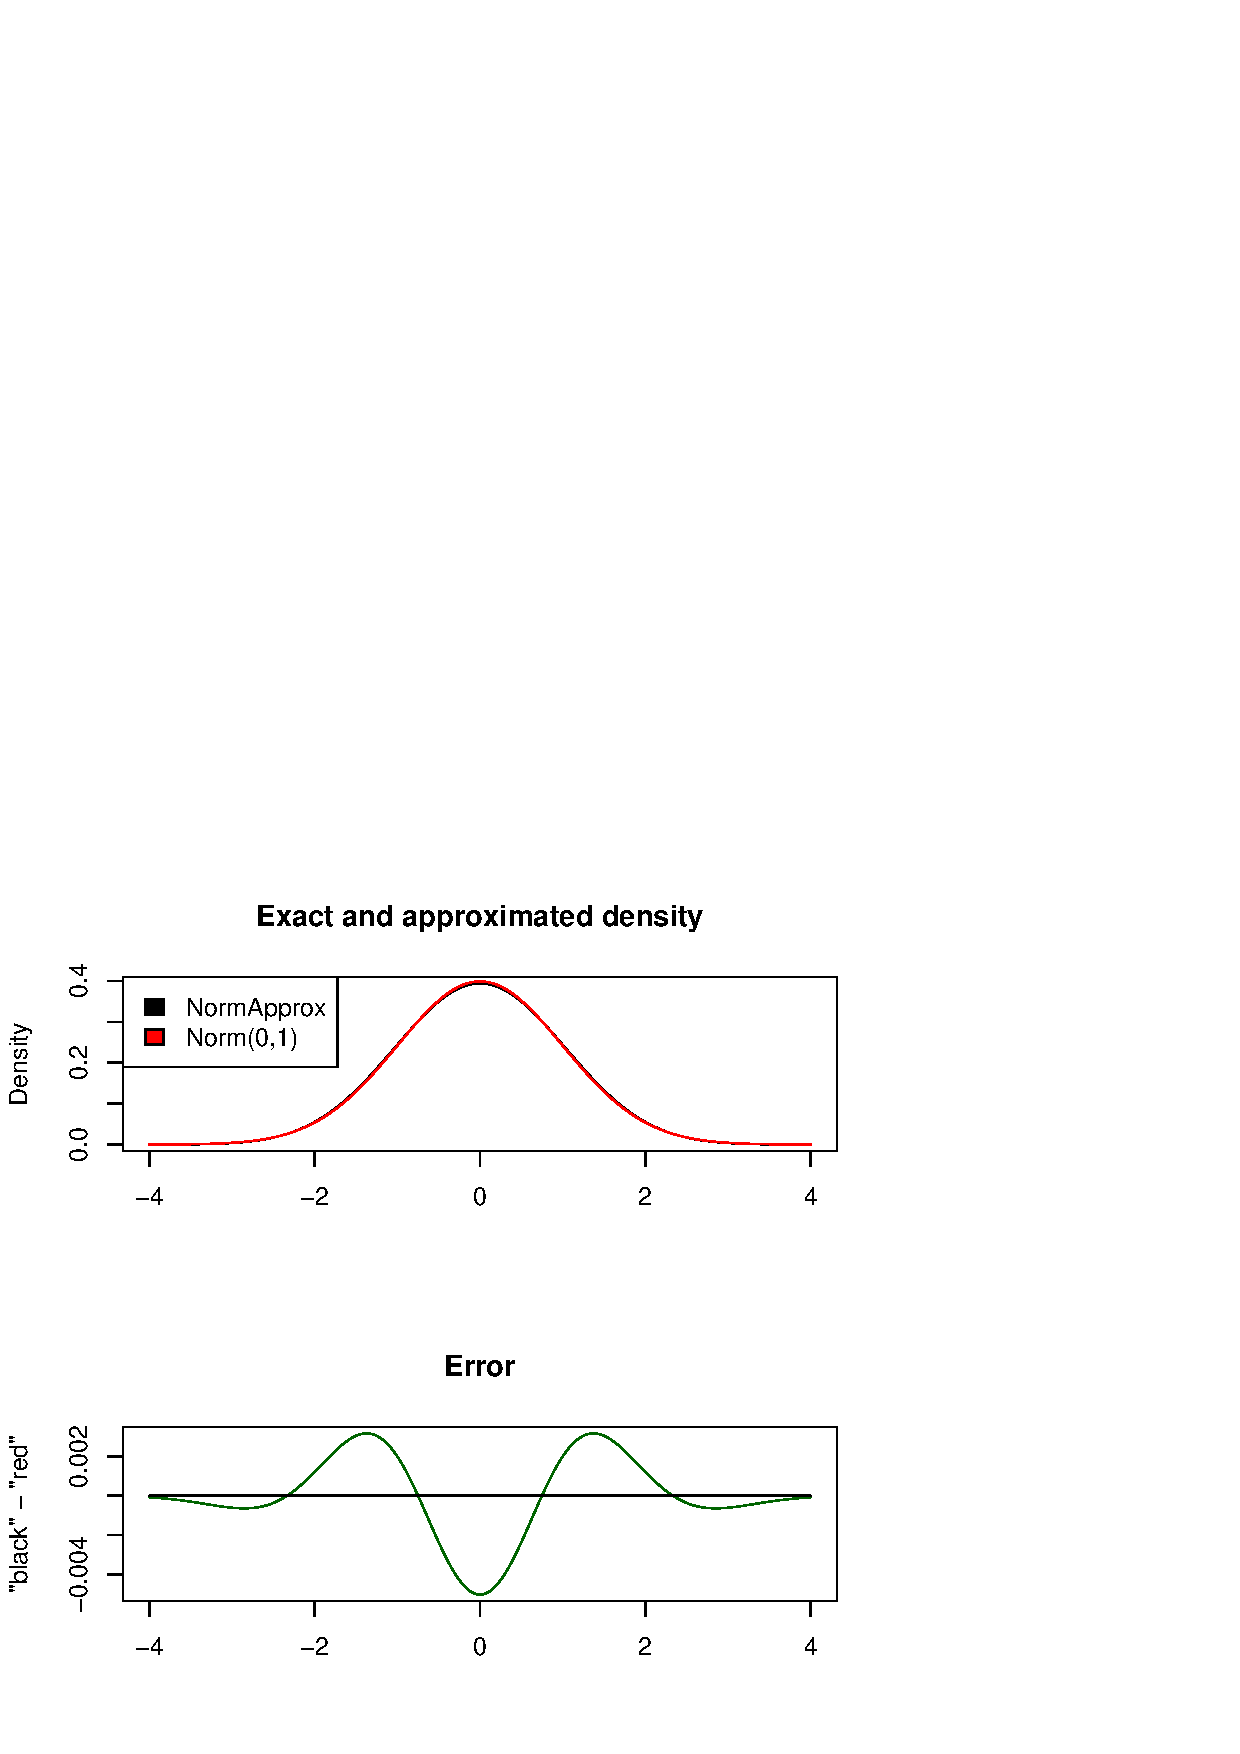
\includegraphics{distr-NormApprox}
\subsection{Comparison of exact convolution to FFT for normal distributions}\label{Convex}
\begin{footnotesize}
  Code also available under\newline \href{http://www.uni-bayreuth.de/departments/math/org/mathe7/DISTR/ConvolutionNormalDistr.R}%
  {\parbox[t]{12cm}{$\mbox{\hspace{2cm}}${\tt http://www.uni-bayreuth.de/departments/math/org/}\\%
  {$\mbox{\hspace{2cm}}$\hphantom{\tt http:/}{\tt /mathe7/DISTR/ConvolutionNormalDistr.R}}}}\\[2ex]
\end{footnotesize}
\begin{small}
  This example illustrates the exactness of the numerical algorithm used to
  compute the convolution: We know that ${\cal L}({\tt A+B})={\cal N}(5,13)$ ---
  if the second argument of ${\cal N}$ is the variance
\end{small}
\begin{Schunk}
\begin{Sinput}
> require(distr)
> ## initialize two normal distributions
> A <- Norm(mean=1, sd=2)
> B <- Norm(mean=4, sd=3)
> ## convolution via addition of moments
> AB <- A+B
> ## casting of A,B as absolutely continuous distributions
> ## that is, ``forget'' that A,B are normal distributions
> A1 <- as(A, "AbscontDistribution")
> B1 <- as(B, "AbscontDistribution")
> ## for higher precision we change the global variable
> ## "TruncQuantile" from 1e-5 to 1e-8
> oldeps <- getdistrOption("TruncQuantile")
> eps <- 1e-8
> distroptions("TruncQuantile" = eps)
> ## support of A1+B1 for FFT convolution is
> ## [q(A1)(TruncQuantile),
> ##  q(B1)(TruncQuantile, lower.tail = FALSE)]
>
> ## convolution via FFT
> AB1 <- A1+B1
> #############################
> ## plots of the results
> #############################
> par(mfrow=c(1,3))
> low <- q(AB)(1e-15)
> upp <- q(AB)(1e-15, lower.tail = FALSE)
> x <- seq(from = low, to = upp, length = 10000)
> ## densities
> plot(x, d(AB)(x), type = "l", lwd = 5)
> lines(x , d(AB1)(x), col = "orange", lwd = 1)
> title("Densities")
> legend("topleft", legend=c("exact", "FFT"),
+         fill=c("black", "orange"))
> ## cdfs
> plot(x, p(AB)(x), type = "l", lwd = 5)
> lines(x , p(AB1)(x), col = "orange", lwd = 1)
> title("CDFs")
> legend("topleft", legend=c("exact", "FFT"),
+         fill=c("black", "orange"))
> ## quantile functions
> x <- seq(from = eps, to = 1-eps, length = 1000)
> plot(x, q(AB)(x), type = "l", lwd = 5)
> lines(x , q(AB1)(x), col = "orange", lwd = 1)
> title("Quantile functions")
> legend("topleft", legend=c("exact", "FFT"),
+         fill=c("black", "orange"))
> ## Since the plots of the results show no
> ## recognizable differencies, we also compute
> ## the total variation distance of the densities
> ## and the Kolmogorov distance of the cdfs
>
> ## total variation distance of densities
> total.var <- function(z, N1, N2){
+     0.5*abs(d(N1)(z) - d(N2)(z))
+ }
> dv <- integrate(total.var, lower=-Inf, upper=Inf, rel.tol=1e-8, N1=AB, N2=AB1)
> cat("Total variation distance of densities:\t")
\end{Sinput}
\begin{Soutput}
Total variation distance of densities:	
\end{Soutput}
\begin{Sinput}
> print(dv) # 4.25e-07
\end{Sinput}
\begin{Soutput}
4.250016e-07 with absolute error < 1.8e-09
\end{Soutput}
\begin{Sinput}
> ### meanwhile realized in package "distrEx"
> ### as TotalVarDist(N1,N2)
>
> ## Kolmogorov distance of cdfs
> ## the distance is evaluated on a random grid
> z <- r(Unif(Min=low, Max=upp))(1e5)
> dk <- max(abs(p(AB)(z)-p(AB1)(z)))
> cat("Kolmogorov distance of cdfs:\t", dk, "\n")
\end{Sinput}
\begin{Soutput}
Kolmogorov distance of cdfs:	 7.269059e-07
\end{Soutput}
\begin{Sinput}
> # 2.03e-07
>
> ### meanwhile realized in package "distrEx"
> ### as KolmogorovDist(N1,N2)
>
> ## old distroptions
> distroptions("TruncQuantile" = oldeps)
\end{Sinput}
\end{Schunk}

\includegraphics{distr-ConvolutionNormalDistr}
\subsection{Comparison of FFT to {\tt RtoDPQ}}\label{compex}
\begin{footnotesize}
  Code also available under\newline \href{http://www.uni-bayreuth.de/departments/math/org/mathe7/DISTR/ComparisonFFTandRtoDPQ.R}%
  {\parbox[t]{12cm}{$\mbox{\hspace{2cm}}${\tt http://www.uni-bayreuth.de/departments/math/org/}\\%
  {$\mbox{\hspace{2cm}}$\hphantom{\tt http:/}{\tt /mathe7/DISTR/ComparisonFFTandRtoDPQ.R}}}}\\[2ex]
\end{footnotesize}
\begin{small}
  This example illustrates the exactness (or rather not--so--exactness) of the
  simulational default algorithm used to compute the distribution of
  transformations of group {\tt math}.
\end{small}
\begin{Schunk}
\begin{Sinput}
> require(distr)
> ################################
> ## Comparison 1 - FFT and RtoDPQ
> ################################
>
> N1 <- Norm(0,3)
> N2 <- Norm(0,4)
> rnew1 <- function(n) r(N1)(n) + r(N2)(n)
> X <- N1 + N2
>      # exact formula -> N(0,5)
> Y <- N1 + as(N2, "AbscontDistribution")
>      # appoximated with FFT
> Z <- new("AbscontDistribution", r = rnew1)
>      # appoximated with RtoDPQ
>
> # density-plot
>
> x <- seq(-15,15,0.01)
> plot(x, d(X)(x),
+      type = "l",
+      lwd = 3,
+      xlab = "",
+      ylab = "density",
+      main = "Comparison 1",
+      col = "black")
> lines(x, d(Y)(x),
+      col = "yellow")
> lines(x, d(Z)(x),
+      col = "red")
> legend("topleft",
+   legend = c("Exact", "FFT-Approximation",
+              "RtoDPQ-Approximation"),
+        fill = c("black", "yellow", "red"))
> ############################################
> ## Comparison 2 - "Exact" Formula and RtoDPQ
> ############################################
>
> B <- Binom(size = 6, prob = 0.5) * 10
> N <- Norm()
> rnew2 <- function(n) r(B)(n) + r(N)(n)
> Y <- B + N
>      # "exact" formula
> Z <- new("AbscontDistribution", r = rnew2)
>      # appoximated with RtoDPQ
>
> # density-plot
>
> x  <- seq(-5,65,0.01)
> plot(x, d(Y)(x),
+      type = "l",
+      xlab = "",
+      ylab = "density",
+      main = "Comparison 2",
+      col = "black")
> lines(x, d(Z)(x),
+      col = "red")
> legend("topleft",
+        legend = c("Exact", "RtoDQP-Approximation"),
+        fill = c("black", "red"))
\end{Sinput}
\end{Schunk}
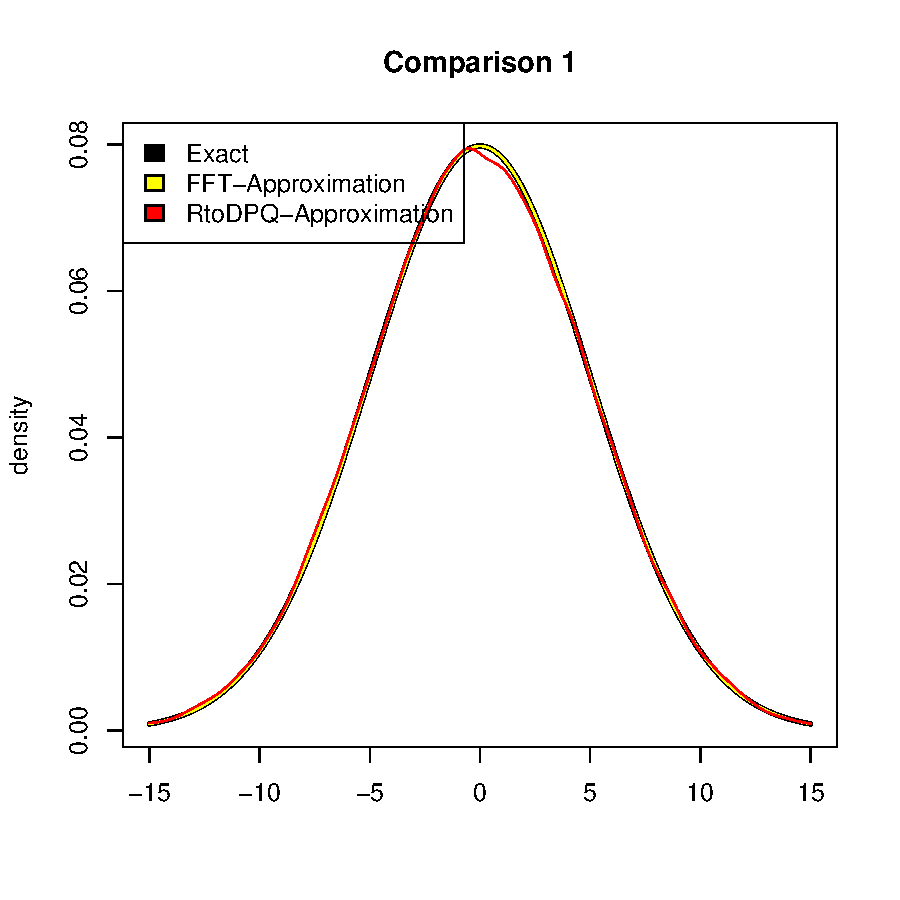
\includegraphics{distr-ComparisonFFTandRtoDPQ}
\subsection{Comparison of exact and approximate stationary regressor distribution}\label{statex}
\begin{footnotesize}
  Code also available under\newline \href{http://www.uni-bayreuth.de/departments/math/org/mathe7/DISTR/StationaryRegressorDistr.R}%
  {\parbox[t]{12cm}{$\mbox{\hspace{2cm}}${\tt http://www.uni-bayreuth.de/departments/math/org/}\\%
  {$\mbox{\hspace{2cm}}$\hphantom{\tt http:/}{\tt /mathe7/DISTR/StationaryRegressorDistr.R}}}}\\[2ex]
\end{footnotesize}
\begin{small}
  Another illustration for the use of package {\tt "distr"}.
  In case of a stationary AR(1)--model, for non--normal innovation distribution,
  the stationary distribution of the observations must be approximated by finite
  convolutions. That these approximations give fairly good results for
  approximations down to small orders is exemplified by the Gaussian case where
  we may compare the approximation to the exact stationary distribution.
\end{small}
\begin{Schunk}
\begin{Sinput}
> require(distr)
> ## Approximation of the stationary regressor
> ## distribution of an AR(1) process
> ##       X_t = phi X_{t-1} + V_t
> ## where V_t i.i.d N(0,1) and phi\in(0,1)
> ## We obtain
> ##    X_t = \sum_{j=1}^\infty phi^j V_{t-j}
> ## i.e., X_t \sim N(0,1/(1-phi^2))
> phi <- 0.5
> ## casting of V as absolutely continuous distributions
> ## that is, ``forget'' that V is a normal distribution
> V <- as(Norm(), "AbscontDistribution")
> ## for higher precision we change the global variable
> ## "TruncQuantile" from 1e-5 to 1e-8
> oldeps <- getdistrOption("TruncQuantile")
> eps <- 1e-8
> distroptions("TruncQuantile" = eps)
> ## Computation of the approximation
> ##      H=\sum_{j=1}^n phi^j V_{t-j}
> ## of the stationary regressor distribution
> ## (via convolution using FFT)
> H <- V
> n <- 15
> ## may take some time
> ### switch off warnings [would be issued due to
> ###  very unequal variances...]
> old.warn <- getOption("warn")
> options("warn" = -1)
> for(i in 1:n){Vi <- phi^i*V; H <- H + Vi }
> options("warn" = old.warn)
> ## the stationary regressor distribution (exact)
> X <- Norm(sd=sqrt(1/(1-phi^2)))
> #############################
> ## plots of the results
> #############################
> par(mfrow=c(1,3))
> low <- q(X)(1e-15)
> upp <- q(X)(1e-15, lower.tail = FALSE)
> x <- seq(from = low, to = upp, length = 10000)
> ## densities
> plot(x, d(X)(x),type = "l", lwd = 5)
> lines(x , d(H)(x), col = "orange", lwd = 1)
> title("Densities")
> legend("topleft", legend=c("exact", "FFT"),
+         fill=c("black", "orange"))
> ## cdfs
> plot(x, p(X)(x),type = "l", lwd = 5)
> lines(x , p(H)(x), col = "orange", lwd = 1)
> title("CDFs")
> legend("topleft", legend=c("exact", "FFT"),
+         fill=c("black", "orange"))
> ## quantile functions
> x <- seq(from = eps, to = 1-eps, length = 1000)
> plot(x, q(X)(x),type = "l", lwd = 5)
> lines(x , q(H)(x), col = "orange", lwd = 1)
> title("Quantile functions")
> legend( "topleft",
+         legend=c("exact", "FFT"),
+         fill=c("black", "orange"))
> ## Since the plots of the results show no
> ## recognizable differencies, we also compute
> ## the total variation distance of the densities
> ## and the Kolmogorov distance of the cdfs
>
> ## total variation distance of densities
> total.var <- function(z, N1, N2){
+     0.5*abs(d(N1)(z) - d(N2)(z))
+ }
> dv <- integrate(f = total.var, lower = -Inf,
+                 upper = Inf, rel.tol = 1e-7,
+                 N1=X, N2=H)
> cat("Total variation distance of densities:\t")
\end{Sinput}
\begin{Soutput}
Total variation distance of densities:	
\end{Soutput}
\begin{Sinput}
> print(dv) # ~ 5.0e-06
\end{Sinput}
\begin{Soutput}
2.091542e-05 with absolute error < 5.8e-08
\end{Soutput}
\begin{Sinput}
> ### meanwhile realized in package "distrEx"
> ### as TotalVarDist(N1,N2)
>
>
> ## Kolmogorov distance of cdfs
> ## the distance is evaluated on a random grid
> z <- r(Unif(Min=low, Max=upp))(1e5)
> dk <- max(abs(p(X)(z)-p(H)(z)))
> cat("Kolmogorov distance of cdfs:\t", dk, "\n")
\end{Sinput}
\begin{Soutput}
Kolmogorov distance of cdfs:	 1.111568e-05
\end{Soutput}
\begin{Sinput}
> # ~2.5e-06
>
> ### meanwhile realized in package "distrEx"
> ### as KolmogorovDist(N1,N2)
>
>
> ## old distroptions
> distroptions("TruncQuantile" = oldeps)
\end{Sinput}
\end{Schunk}
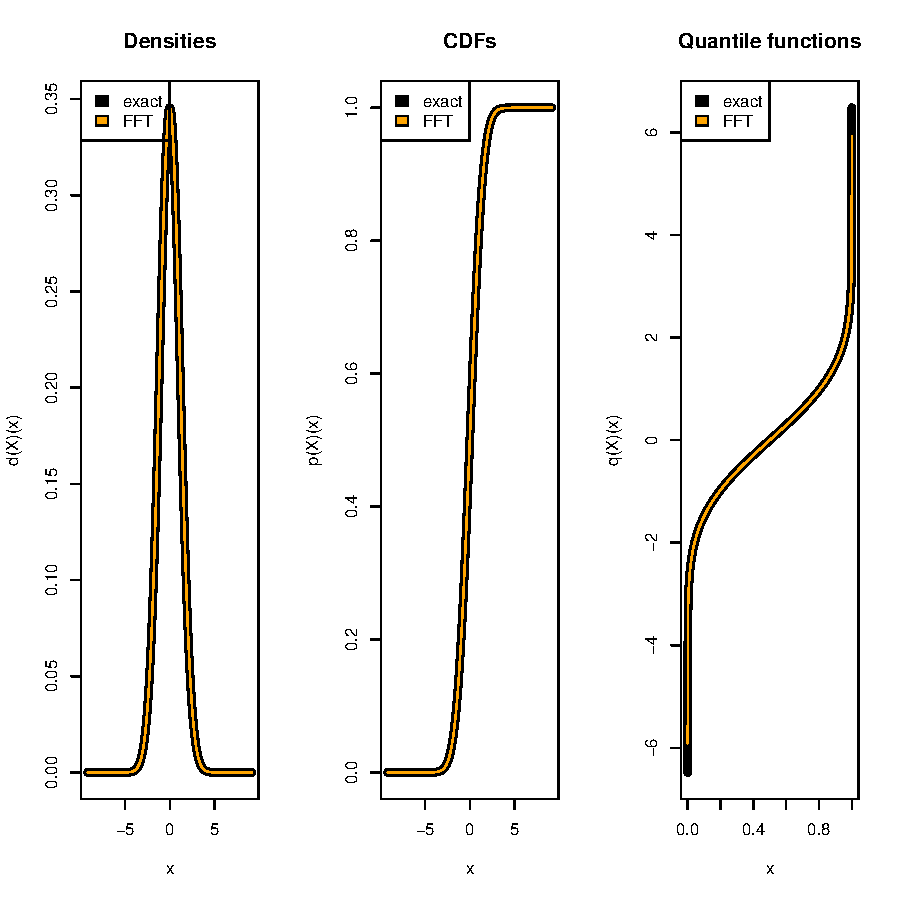
\includegraphics{distr-StationaryRegressorDistr}
\subsection{Truncation and Huberization/winsorization}\label{truncex}
has been integrated to the package itself, see section~\ref{TruncMin}
\subsection{Distribution of minimum and maximum of two independent random variables}\label{minmaxex}
has been integrated to the package itself, see section~\ref{TruncMin}
\subsection{Instructive destructive example}\label{destrex}
\begin{footnotesize}
  Code also available under\newline \href{http://www.uni-bayreuth.de/departments/math/org/mathe7/DISTR/destructive.R}%
  {\parbox[t]{12cm}{$\mbox{\hspace{2cm}}${\tt http://www.uni-bayreuth.de/departments/math/org/}\\%
  {$\mbox{\hspace{2cm}}$\hphantom{\tt http:/}{\tt /mathe7/DISTR/destructive.R}}}}\\[2ex]
\end{footnotesize}
\begin{Schunk}
\begin{Sinput}
> ##########################################################
> ## Demo: Instructive destructive example
> ##########################################################
> require(distr)
> ## package "distr" encourages
> ## consistency but does not
> ## enforce it---so in general
> ## d o   n o t   m o d i f y
> ## slots d,p,q,r!
>
> N <- Norm()
> B <- Binom()
> N@d <- B@d
> plot(N, lwd = 3, withSweave = TRUE)
\end{Sinput}
\end{Schunk}
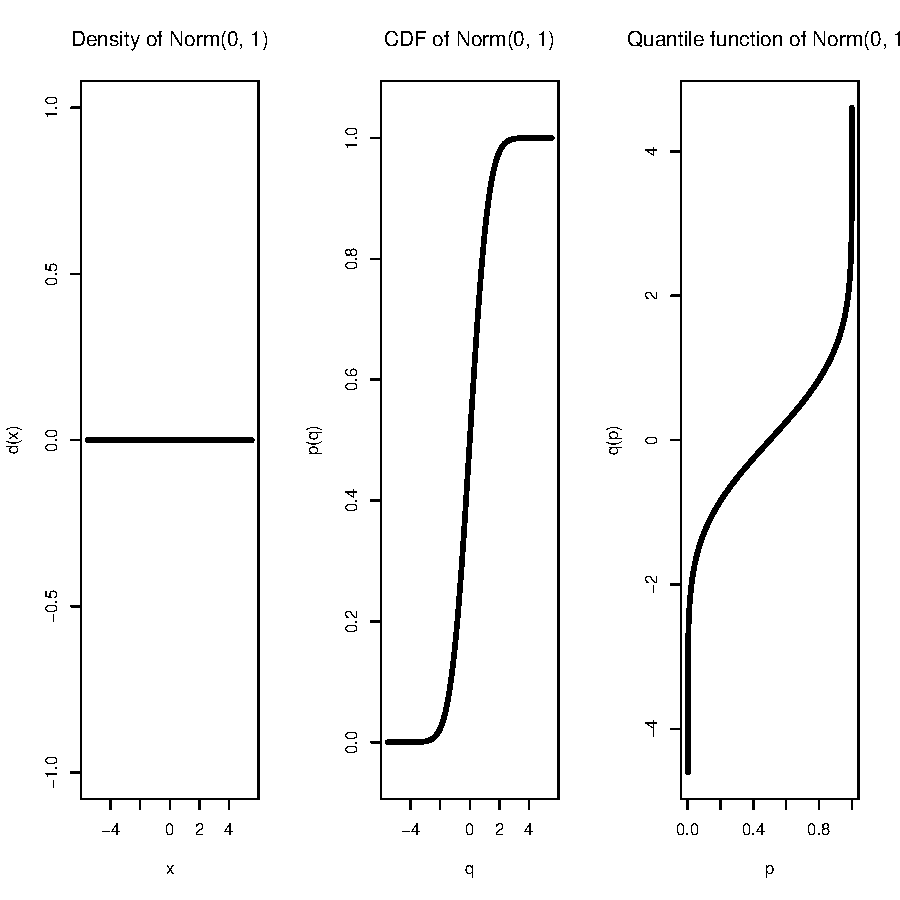
\includegraphics{distr-destructive}
\subsection{A simulation example}\label{simex}
{\bf needs packages \pkg{distrSim}/\pkg{distrTEst}}\\[2ex]
\begin{footnotesize}
  Code also available under\newline \href{http://www.uni-bayreuth.de/departments/math/org/mathe7/DISTR/SimulateandEstimate.R}%
  {\parbox[t]{12cm}{$\mbox{\hspace{2cm}}${\tt http://www.uni-bayreuth.de/departments/math/org/}\\%
  {$\mbox{\hspace{2cm}}$\hphantom{\tt http:/}{\tt /mathe7/DISTR/SimulateandEstimate.R}}}}\\[2ex]
\end{footnotesize}
\begin{Schunk}
\begin{Sinput}
> have.distrTEst <- suppressWarnings(require(distrTEst))
>     ### also loads distrSim
> if (have.distrTEst)
+    { sim <- new("Simulation",
+                 seed = setRNG(),
+                 distribution = Norm(mean = 0, sd = 1),
+                 filename="sim_01",
+                 runs = 1000,
+                 samplesize = 30)
+
+      contsim <- new("Contsimulation",
+                     seed = setRNG(),
+                     distribution.id = Norm(mean = 0, sd = 1),
+                     distribution.c = Norm(mean = 0, sd = 9),
+                     rate = 0.1,
+                     filename="contsim_01",
+                     runs = 1000,
+                     samplesize = 30)
+
+      simulate(sim)
+      simulate(contsim)
+
+      print(sim)
+      summary(contsim)
+      plot(contsim)
+    } else {
+     cat("\n functionality not (yet) available; ")
+     cat("you have to install package \"distrTEst\" first.\n")
+    }
\end{Sinput}
\begin{Soutput}
filename of Simulation: sim_01
Seed:  Kind: Mersenne-Twister
       Normal Kind: Inversion
       first 6 numbers:  1925048547	-2062600733	 0958297670
                         1485015887	-0735449209	-2018507072
number of runs: 1000
dimension of the observations: 1
size of sample: 30
object was generated by version: 1.9
Distribution:
Distribution Object of Class: Norm
 mean: 0
 sd: 1
name of simulation: contsim_01
rate of contamination: 0.100000
real Data:
dimension of the observations: 1
number of runs: 1000
size of sample: 30
\end{Soutput}
\end{Schunk}
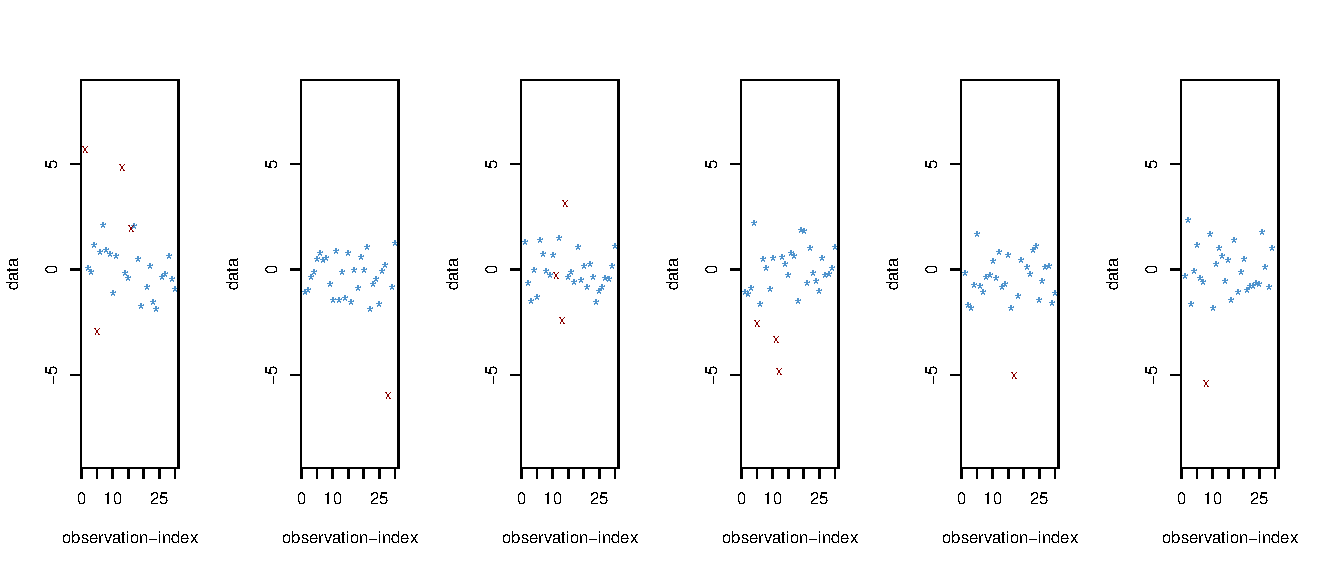
\includegraphics{distr-SimulateandEstimate}
\begin{Schunk}
\begin{Sinput}
> have.distrTEst <- suppressWarnings(require("distrTEst"))
> if (have.distrTEst)
+    { psim <- function(theta,y,m0){
+        mean(pmin(pmax(-m0, y - theta), m0))
+        }
+      mestimator <- function(x, m = 0.7) {
+        uniroot(f = psim,
+                lower = -20,
+                upper = 20,
+                tol = 1e-10,
+                y = x,
+                m0 = m,
+                maxiter = 20)$root
+        }
+
+      result.id.mean <- evaluate(sim, mean)
+      result.id.mest <- evaluate(sim, mestimator)
+      result.id.median <- evaluate(sim, median)
+
+
+      result.cont.mean <- evaluate(contsim, mean)
+      result.cont.mest <- evaluate(contsim, mestimator)
+      result.cont.median <- evaluate(contsim, median)
+
+      elist <- EvaluationList(result.cont.mean,
+                              result.cont.mest,
+                              result.cont.median)
+
+      print(elist)
+      summary(elist)
+      plot(elist, cex = 0.7, las = 2)
+    } else {
+     cat("\n functionality not (yet) available; ")
+     cat("you have to install package \"distrTEst\" first.\n")
+    }
\end{Sinput}
\begin{Soutput}
An EvaluationList Object
name of Evaluation List: a list of "Evaluation" objects
name of Dataobject: object
name of Datafile: contsim_01
----------------------------------
An Evaluation Object
estimator: mean
Result: 'data.frame':	1000 obs. of  2 variables:
 $ mean.id: num   0.00598  0.00162 -0.10094  0.08660  0.50101 ...
 $ mean.re: num   0.1453 -0.7871  0.2827  0.0849 -0.2064 ...
----------------------------------
An Evaluation Object
estimator: mestimator
Result: 'data.frame':	1000 obs. of  2 variables:
 $ mstm.id: num  -0.0278 -0.0137 -0.1697  0.0501  0.4922 ...
 $ mstm.re: num  -0.0717 -0.0495 -0.2060  0.0136  0.4148 ...
----------------------------------
An Evaluation Object
estimator: median
Result: 'data.frame':	1000 obs. of  2 variables:
 $ medn.id: num  -0.0896  0.0800 -0.3559  0.0360  0.6089 ...
 $ medn.re: num  -0.2811  0.0800 -0.2738  0.0360  0.4185 ...
name of Evaluation List: a list of "Evaluation" objects
name of Dataobject: object
name of Datafile: contsim_01
----------------------------------
name of Evaluation: object
estimator: mean
Result:
    mean.id             mean.re
 Min.   :-0.596862   Min.   :-1.930618
 1st Qu.:-0.120672   1st Qu.:-0.357320
 Median :-0.007168   Median : 0.002932
 Mean   :-0.001907   Mean   :-0.003301
 3rd Qu.: 0.126348   3rd Qu.: 0.349952
 Max.   : 0.641179   Max.   : 1.839373
----------------------------------
name of Evaluation: object
estimator: mestimator
Result:
    mstm.id             mstm.re
 Min.   :-0.581245   Min.   :-0.745974
 1st Qu.:-0.138264   1st Qu.:-0.164353
 Median :-0.012663   Median :-0.002387
 Mean   :-0.002162   Mean   :-0.001195
 3rd Qu.: 0.128317   3rd Qu.: 0.142610
 Max.   : 0.635923   Max.   : 0.938872
----------------------------------
name of Evaluation: object
estimator: median
Result:
    medn.id             medn.re
 Min.   :-0.814394   Min.   :-8.485e-01
 1st Qu.:-0.153502   1st Qu.:-1.718e-01
 Median :-0.008341   Median :-3.236e-03
 Mean   :-0.001774   Mean   :-8.367e-05
 3rd Qu.: 0.147806   3rd Qu.: 1.644e-01
 Max.   : 0.916559   Max.   : 9.617e-01
\end{Soutput}
\end{Schunk}
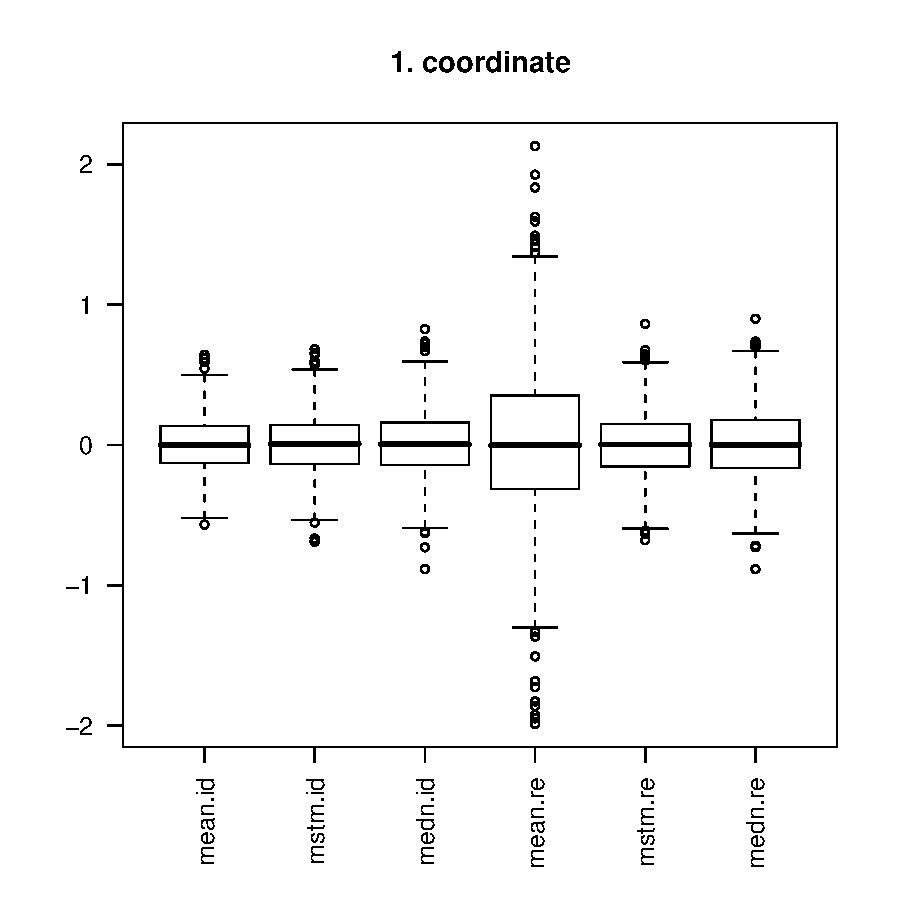
\includegraphics{distr-elist}
\par
\begin{footnotesize}
Output by \code{plot}/\code{show}-method for an object of class \code{Evaluation}
\begin{Schunk}
\begin{Sinput}
> result.cont.mest
\end{Sinput}
\begin{Soutput}
An Evaluation Object
name of Dataobject: object
name of Datafile: contsim_01
estimator: mestimator
Result: 'data.frame':	1000 obs. of  2 variables:
 $ mstm.id: num  -0.0278 -0.0137 -0.1697  0.0501  0.4922 ...
 $ mstm.re: num  -0.0717 -0.0495 -0.2060  0.0136  0.4148 ...
\end{Soutput}
\end{Schunk}
\end{footnotesize}
\begin{footnotesize}
Output by \code{summary}-method for an object of class \code{EvaluationList}
\begin{Schunk}
\begin{Sinput}
> summary(elist)
\end{Sinput}
\begin{Soutput}
name of Evaluation List: a list of "Evaluation" objects
name of Dataobject: object
name of Datafile: contsim_01
----------------------------------
name of Evaluation: object
estimator: mean
Result:
    mean.id             mean.re
 Min.   :-0.596862   Min.   :-1.930618
 1st Qu.:-0.120672   1st Qu.:-0.357320
 Median :-0.007168   Median : 0.002932
 Mean   :-0.001907   Mean   :-0.003301
 3rd Qu.: 0.126348   3rd Qu.: 0.349952
 Max.   : 0.641179   Max.   : 1.839373
----------------------------------
name of Evaluation: object
estimator: mestimator
Result:
    mstm.id             mstm.re
 Min.   :-0.581245   Min.   :-0.745974
 1st Qu.:-0.138264   1st Qu.:-0.164353
 Median :-0.012663   Median :-0.002387
 Mean   :-0.002162   Mean   :-0.001195
 3rd Qu.: 0.128317   3rd Qu.: 0.142610
 Max.   : 0.635923   Max.   : 0.938872
----------------------------------
name of Evaluation: object
estimator: median
Result:
    medn.id             medn.re
 Min.   :-0.814394   Min.   :-8.485e-01
 1st Qu.:-0.153502   1st Qu.:-1.718e-01
 Median :-0.008341   Median :-3.236e-03
 Mean   :-0.001774   Mean   :-8.367e-05
 3rd Qu.: 0.147806   3rd Qu.: 1.644e-01
 Max.   : 0.916559   Max.   : 9.617e-01
\end{Soutput}
\end{Schunk}
\end{footnotesize}
\begin{small}
In this example we present a standard robust simulation study that --- in variations --- arises in almost
every paper on Robust Statistics. We do this with the tools provided by our package\ldots
\end{small}
\subsection{Expectation of a given function under a given distribution}
\begin{footnotesize}
  Code also available under\newline \href{http://www.uni-bayreuth.de/departments/math/org/mathe7/DISTR/Expectation.R}%
  {\parbox[t]{12cm}{$\mbox{\hspace{2cm}}${\tt http://www.uni-bayreuth.de/departments/math/org/}\\%
  {$\mbox{\hspace{2cm}}$\hphantom{\tt http:/}{\tt /mathe7/DISTR/Expectation.R}}}}\\[2ex]
  This code is for illustration only; in the mean-time, the expectation- and
  variance operators implemented in this example have been included to package
   \pkg{distrEx} where their functionality has further been extended.
\end{footnotesize}
\begin{small}
As in examples~\ref{truncex} and \ref{minmaxex}, we illustrate the use of
package {\tt "distr"} by implementing a general evaluation of expectation
and variance under a given distribution.
\end{small}
\begin{Schunk}
\begin{Sinput}
> have.distrEx <- suppressWarnings(require("distrEx"))
> if (have.distrEx)
+    {
+      # Example
+      id <- function(x) x
+      sq <- function(x) x^2
+
+      # Expectation and Variance of Binom(6,0.5)
+      B <- Binom(6, 0.5)
+      print(E(B, id))
+      print(E(B, sq) - E(B, id)^2)
+
+      # Expectation and Variance of Norm(1,1)
+      N <- Norm(1, 1)
+      print(E(N, id))
+      print(E(N, sq) - E(N, id)^2)
+    } else {
+     cat("\n functionality not (yet) available; ")
+     cat("you have to install package \"distrEx\" first.\n")
+    }
\end{Sinput}
\begin{Soutput}
[1] 3
[1] 1.5
[1] 0.9999998
[1] 0.9999944
\end{Soutput}
\end{Schunk}
\subsection{$n$-fold convolution of absolutely continuous distributions}\label{exe10}
\begin{footnotesize}
  Code also available under\newline \href{http://www.uni-bayreuth.de/departments/math/org/mathe7/DISTR/nFoldConvolution.R}%
  {\parbox[t]{12cm}{$\mbox{\hspace{2cm}}${\tt http://www.uni-bayreuth.de/departments/math/org/}\\%
  {$\mbox{\hspace{2cm}}$\hphantom{\tt http:/}{\tt /mathe7/DISTR/nFoldConvolution.R}}}}\\[2ex]
\end{footnotesize}
\begin{small}
Might be useful for teaching the CLT: a straightforward implementation of the
$n$--fold convolution of an
arbitrary implemented absolutely continuous distribution --- to show accuracy
of our method we compare it to the
exact formula valid for $n$-fold convolution of normal distributions.\\
From version 1.9 this is integrated to package \pkg{distr}.
\end{small}
\begin{Schunk}
\begin{Sinput}
> ##########################################################
> ## Demo: n-fold convolution of absolutely continuous
> ##       probability distributions
> ##########################################################
> require(distr)
> if(!isGeneric("convpow"))
+     setGeneric("convpow",
+     function(D1,...) standardGeneric("convpow"))
> ##########################################################
> ## Function for n-fold convolution
> ## -- absolute continuous distribution --
> ##########################################################
>
> ##implentation of Algorithm 3.4. of
> # Kohl, M., Ruckdeschel, P., Stabla, T. (2005):
> #   General purpose convolution algorithm for distributions
> #   in S4-Classes by means of FFT.
> # Technical report, Feb. 2005. Also available in
> # http://www.uni-bayreuth.de/departments/math/org/mathe7/
> #       /RUCKDESCHEL/pubs/comp.pdf
>
>
> setMethod("convpow",
+           signature(D1 = "AbscontDistribution"),
+           function(D1, N){
+             if((N < 1)||(!identical(floor(N), N)))
+               stop("N has to be a natural greater than 0")
+
+             m <- getdistrOption("DefaultNrFFTGridPointsExponent")
+
+     ##STEP 1
+
+             lower <- ifelse((q(D1)(0) > - Inf), q(D1)(0),
+                      q(D1)(getdistrOption("TruncQuantile")))
+             upper <- ifelse((q(D1)(1) < Inf), q(D1)(1),
+                      q(D1)(getdistrOption("TruncQuantile"), lower.tail = FALSE))
+
+     ##STEP 2
+
+             M <- 2^m
+             h <- (upper-lower)/M
+             if(h > 0.01)
+               warning(paste("Grid for approxfun too wide, ",
+               "increase DefaultNrFFTGridPointsExponent", sep=""))
+             x <- seq(from = lower, to = upper, by = h)
+             p1 <- p(D1)(x)
+
+     ##STEP 3
+
+             p1 <- p1[2:(M + 1)] - p1[1:M]
+
+     ##STEP 4
+
+             ## computation of DFT
+             pn <- c(p1, numeric((N-1)*M))
+             fftpn <- fft(pn)
+
+     ##STEP 5
+
+             ## convolution theorem for DFTs
+             pn <- Re(fft(fftpn^N, inverse = TRUE)) / (N*M)
+             pn <- (abs(pn) >= .Machine$double.eps)*pn
+             i.max <- N*M-(N-2)
+             pn <- c(0,pn[1:i.max])
+             dn <- pn / h
+             pn <- cumsum(pn)
+
+     ##STEP 6(density)
+
+             ## density
+             x <- c(N*lower,seq(from = N*lower+N/2*h,
+                    to = N*upper-N/2*h, by=h),N*upper)
+             dnfun1 <- approxfun(x = x, y = dn, yleft = 0, yright = 0)
+
+     ##STEP 7(density)
+
+             standardizer <- sum(dn[2:i.max]) + (dn[1]+dn[i.max+1]) / 2
+             dnfun2 <- function(x) dnfun1(x) / standardizer
+
+     ##STEP 6(cdf)
+
+             ## cdf with continuity correction h/2
+             pnfun1 <- approxfun(x = x+0.5*h, y = pn,
+                         yleft = 0, yright = pn[i.max+1])
+
+     ##STEP 7(cdf)
+
+             pnfun2 <- function(x) pnfun1(x) / pn[i.max+1]
+
+
+             ## quantile with continuity correction h/2
+             yleft <- ifelse(((q(D1)(0) == -Inf)|
+                              (q(D1)(0) == -Inf)),
+                              -Inf, N*lower)
+             yright <- ifelse(((q(D1)(1) == Inf)|
+                               (q(D1)(1) == Inf)),
+                               Inf, N*upper)
+             w0 <- options("warn")
+             options(warn = -1)
+             qnfun1 <- approxfun(x = pnfun2(x+0.5*h),
+                         y = x+0.5*h, yleft = yleft, yright = yright)
+             qnfun2 <- function(x){
+             ind1 <- (x == 0)*(1:length(x))
+             ind2 <- (x == 1)*(1:length(x))
+             y <- qnfun1(x)
+             y <- replace(y, ind1[ind1 != 0], yleft)
+             y <- replace(y, ind2[ind2 != 0], yright)
+             return(y)
+             }
+             options(w0)
+
+             rnew = function(N) apply(matrix(r(e1)(n*N),
+                                      ncol=N), 1, sum)
+
+             return(new("AbscontDistribution", r = rnew,
+                        d = dnfun1, p = pnfun2, q = qnfun2))
+ })
\end{Sinput}
\begin{Soutput}
[1] "convpow"
\end{Soutput}
\begin{Sinput}
> ## initialize a normal distribution
> A <- Norm(mean=0, sd=1)
> ## convolution power
> N <- 10
> ## convolution via FFT
> AN <- convpow(as(A,"AbscontDistribution"), N)
> ##  ... for the normal distribution , 'convpow' has an "exact"
> ##      method by version 1.9 so the as(.,.)  is needed to
> ##      see how the algorithm above works
>
> ## convolution exact
> AN1 <- Norm(mean=0, sd=sqrt(N))
> ## plots of the results
> eps <- getdistrOption("TruncQuantile")
> par(mfrow=c(1,3))
> low <- q(AN1)(eps)
> upp <- q(AN1)(eps, lower.tail = FALSE)
> x <- seq(from = low, to = upp, length = 10000)
> ## densities
> plot(x, d(AN1)(x), type = "l", lwd = 5)
> lines(x , d(AN)(x), col = "orange", lwd = 1)
> title("Densities")
> legend("topleft", legend=c("exact", "FFT"),
+         fill=c("black", "orange"))
> ## cdfs
> plot(x, p(AN1)(x), type = "l", lwd = 5)
> lines(x , p(AN)(x), col = "orange", lwd = 1)
> title("CDFs")
> legend("topleft", legend=c("exact", "FFT"),
+         fill=c("black", "orange"))
> ## quantile functions
> x <- seq(from = eps, to = 1-eps, length = 1000)
> plot(x, q(AN1)(x), type = "l", lwd = 5)
> lines(x , q(AN)(x), col = "orange", lwd = 1)
> title("Quantile functions")
> legend("topleft",
+        legend = c("exact", "FFT"),
+         fill = c("black", "orange"))
\end{Sinput}
\end{Schunk}
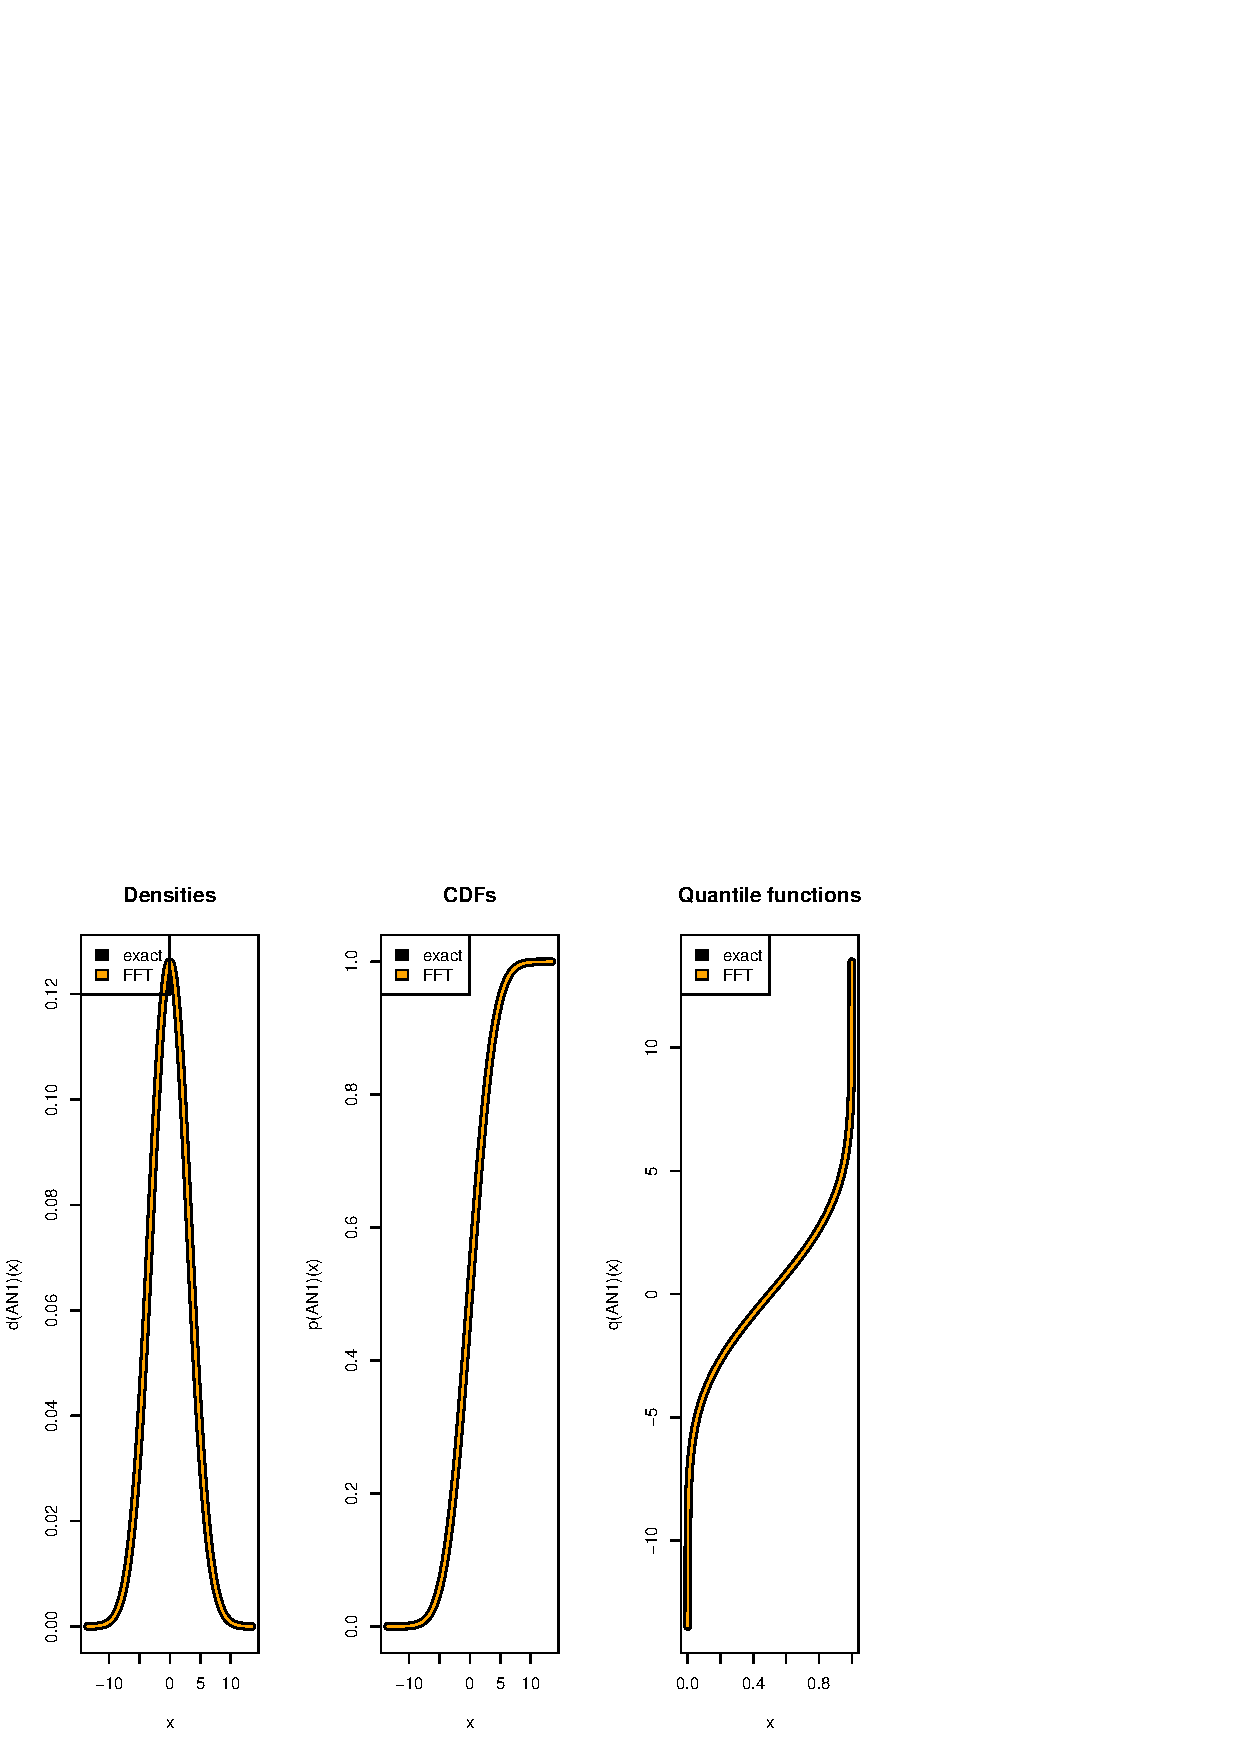
\includegraphics{distr-nFoldConvolution}
%-------------------------------------------------------------------------------
\begin{thebibliography}{8}

\bibitem{Beng:03}
Bengtsson H.
\newblock The {R.oo} package - object-oriented programming with references using
standard {R} code.
\newblock In: Hornik K., Leisch F. and Zeileis A. (Eds.) {\em
  Proceedings of the 3rd International Workshop on Distributed Statistical
  Computing (DSC 2003)\/}. Vienna, Austria.
\newblock Published as http://www.ci.tuwien.ac.at/Conferences/DSC-2003/

\bibitem{Cham:98}
Chambers J.M.
\newblock {\em {Programming with data. A guide to the S language}\/}.
\newblock {Springer}.
\newblock http://cm.bell-labs.com/stat/Sbook/index.html

\bibitem{OOPGent}
Gentleman R.
\newblock {\em Object Orientated Programming. Slides of a Short Course held in
Auckland\/}.
\newblock http://www.stat.auckland.ac.nz/S-Workshop/Gentleman/Methods.pdf

\bibitem{MK:05}
Kohl M.
\newblock {\em Numerical Contributions to the Asymptotic Theory of Robustness\/}.
\newblock {Dissertation}, Universit\"at Bayreuth.
\newblock See also http://stamats.de/ThesisMKohl.pdf

\bibitem{K:R:S:04}
Kohl M., Ruckdeschel P. and Stabla T.
\newblock {General Purpose Convolution Algorithm for Distributions in S4-Classes
by means of FFT}.
\newblock unpublished manual

\bibitem{NumR:92}
Press W.H., Teukolsky S.A., Vetterling W.T. and Flannery B.P.
\newblock {\em {Numerical recipes in C. The art of scientific computing.}\/}
\newblock {Cambridge Univ. Press}, 2. Aufl.

\bibitem{Ric:88}
Rice J.A.
\newblock {\em {Mathematical statistics and data analysis}\/}.
\newblock The Wadsworth \& Brooks/Cole Statistics/Probability Series.
  {Wadsworth \& Brooks/Cole Advanced Books \& Software}, Pacific Grove,
  California.

\bibitem{R:K:S:C:04}
Ruckdeschel P., Kohl M., Stabla T., and Camphausen F.
\newblock {S4 Classes for Distributions.}
\newblock {\em R-News\/}, {\bf 6}(2): 10--13.
\newblock http://CRAN.R-project.org/doc/Rnews/Rnews\_2006-2.pdf
%\newblock See also {http://www.uni-bayreuth.de/departments/math/org/mathe7/RUCKDESCHEL/pubs/distr.pdf}

\end{thebibliography}
% -------------------------------------------------------------------------------
\end{document}
% -------------------------------------------------------------------------------
